\documentclass[UTF8,letterpaper,zihao=5,twocolumn]{ctexart}

\usepackage[letterpaper,top=0.68in,bottom=0.72in,left=0.68in,right=0.68in]{geometry}
\usepackage{amsmath,amssymb,amsfonts}
\usepackage{graphicx}
\usepackage{booktabs}
\usepackage{multirow}
\usepackage{tabularx}
\usepackage{longtable}
\usepackage{siunitx}
\usepackage{algorithm}
\usepackage{algpseudocode}
\usepackage{caption}
\usepackage{subcaption}
\usepackage{dblfloatfix}
\usepackage[numbers,sort&compress]{natbib}
\usepackage[colorlinks=true,linkcolor=blue,citecolor=blue,urlcolor=blue]{hyperref}
\usepackage[nameinlink,noabbrev]{cleveref}

\graphicspath{{figures/}}
\setlength{\columnsep}{0.24in}
\setlength{\parindent}{1em}
\setlength{\parskip}{0pt}
\setlength{\floatsep}{8pt plus 2pt minus 2pt}
\setlength{\textfloatsep}{9pt plus 2pt minus 2pt}
\setlength{\intextsep}{8pt plus 2pt minus 2pt}
\setlength{\abovecaptionskip}{3pt}
\setlength{\belowcaptionskip}{0pt}
\captionsetup{font=small,labelfont=bf}
\captionsetup[sub]{font=footnotesize}
\renewcommand{\topfraction}{0.9}
\renewcommand{\bottomfraction}{0.85}
\renewcommand{\textfraction}{0.08}
\renewcommand{\floatpagefraction}{0.88}
\renewcommand{\dbltopfraction}{0.9}
\renewcommand{\dblfloatpagefraction}{0.9}
\setcounter{topnumber}{4}
\setcounter{bottomnumber}{2}
\setcounter{totalnumber}{6}
\setcounter{dbltopnumber}{4}
\emergencystretch=2em

\title{面向强约束三维无人机路径规划的约束可行性场驱动进化搜索}
\author{作者、单位与通讯作者信息待补}
\date{\today}

\begin{document}

\maketitle

\begin{abstract}
强约束低空无人机路径规划需要在障碍物、禁飞区、高度边界和路径平滑性等条件下同时形成可行且稳定的三维轨迹。针对基础进化搜索在窄可行走廊中容易产生不可行个体、低质量绕行和边界贴靠的问题，本文构建一种约束可行性场驱动的自适应进化搜索方法（CVF-AE）。该方法将约束违反信息前移为候选生成阶段的有界方向修正，并通过状态调度、稀疏触发和保守局部接收限制 CVF 的作用范围，避免全种群强制场更新。基于三类合成低空三维场景的实验表明，在所选代表性基线中，CVF-AE 保持 $1.00$ 的可行率，并取得最佳平均排名，在工程轨迹复核标记和额外评价开销之间保持较好折中；消融结果进一步验证了 CVF 候选方向与初始化、稀疏可行性保持机制的互补作用。评价开销分析显示，CVF 分支触发率低于 $1\%$，额外评价次数约为 $1\%$ 量级。结果说明，CVF-AE 可作为静态合成强约束低空路径规划中的均衡型候选生成框架。
\end{abstract}

\noindent\textbf{关键词：} 无人机路径规划；约束优化；进化算法；约束可行性场；启发式优化

\section{引言}
\label{sec:introduction}

低空无人机在巡检、监测、配送和应急响应等任务中具有部署灵活和快速到达的优势。在建筑密集、禁飞区交错且风险分布不均的低空空间中，路径规划需要同时权衡障碍物避让、禁飞区规避、高度边界、转弯平滑性、风险暴露和能耗，而非仅寻找一条短路径。已有综述将 UAV 路径规划概括为图搜索、采样、数学规划、智能优化、学习和混合等多类路线，并指出复杂环境中的三维可行性保持与多约束折中仍是核心问题 \citep{Kumar2025UAVReview,Ghambari2024UAVSurvey}。

围绕复杂约束下的搜索效率与路径质量，同行已从初始化、候选生成、更新和局部引导等环节提出改进。Darlan 等将 A* 引导的交叉、变异和自适应多项式变异嵌入进化算法 \citep{Darlan2026DomainSpecificEA}；Niu 等在连续蚁群优化中结合随机游走和自适应路径点修复 \citep{Niu2025ContinuousACO}；Chen 等面向多 UAV 威胁环境，将偏置采样、候选评价和路径重构整合到 RRT* 框架 \citep{Chen2025BiasedSampling}；Wang 等在多目标水母搜索中利用 RRT 初始化和类别最优个体引导改善初始路径与搜索压力 \citep{Wang2024JellyfishUAV}；Meng 等则通过自适应算子选择和知识融合增强进化多任务路径搜索 \citep{Meng2025EvoMultitasking}。在局部方向引导方面，Khatib 提出了经典人工势场思想 \citep{Khatib1986PotentialField}，Liu 等进一步以旋转势场和参数学习服务多 UAV 协同规划 \citep{Liu2025RotationAPF}。这些研究说明领域知识可以有效参与搜索，但本文所面对的痛点不同：对于单条强约束 B 样条路径，惩罚项和 Deb 规则只能在候选评价后识别不可行性；而若将局部方向强制施加给全种群，又可能干扰基础进化搜索。因此，需要一种能够在评价前提供局部约束方向、按群体状态稀疏介入，并以保守规则限制替换范围的候选生成机制。

针对上述不足，本文提出约束可行性场驱动的自适应进化搜索方法（Constraint Viability Field guided Adaptive Evolution, CVF-AE）。本文不以 CVF 替代基础 AE 或构造新的目标函数，而是将其设计为候选生成中的局部修正机制：约束感知初始化和参考弱引导首先帮助种群进入潜在可行走廊；形成、保持和恢复三种状态根据群体可行性与搜索进展决定何时介入；对少量近可行候选，CVF 将障碍物、禁飞区、风险、高度、边界和转弯信息编码为有界控制点增量；候选仅在 Deb 顺序改善且含惩罚综合适应度不增加时才被保留。由此，初始化、状态调度、场构建和保守接收共同构成一个在不接管全局搜索前提下前移约束信息的闭环。基于这一思路，本文的贡献如下：

\begin{itemize}
    \item 提出面向 B 样条控制点编码的 CVF 表示，将障碍物、禁飞区、高度与边界等局部约束信息，以及风险和转弯等质量信息，映射为控制点层面的有界方向增量，使局部信息在候选评价前参与搜索，而不只通过目标项和惩罚项事后体现。
    \item 设计以“进入--介入--移动”为主线的稀疏候选增强框架：约束感知初始化提供弱先验，三状态调度和近可行触发决定介入时机与对象，基础 AE 方向与 CVF 方向在受限步长内融合，从而保留全局进化搜索的主体地位。
    \item 给出“接受--替换”的保守边界：CVF 候选经过边界投影后，须同时满足局部 Deb 优先和含惩罚综合适应度不增条件才可替代基础候选；稀疏可行性保持仅作用于少量候选，以避免将局部修正扩展为全种群强制修复。
\end{itemize}

本文其余部分组织如下：第 \ref{sec:problem-formulation} 节给出路径编码、目标函数、约束违反量和可行性准则；第 \ref{sec:method} 节介绍 CVF-AE 的候选生成、约束状态识别、CVF 构建和稀疏触发机制；第 \ref{sec:results-discussion} 节依次说明整体实验设置、主对比、消融、显著性和开销分析，并在相应小节内讨论结果含义与方法边界；最后给出结论。

% 相关工作内容已并入第 \ref{sec:introduction} 节，保留该文件以维持 main.tex 的输入结构。

\section{问题建模}

\label{sec:problem-formulation}

本文研究强约束三维低空无人机路径规划问题。给定三维飞行空间、起点、终点、障碍物、禁飞区和高度约束，目标是在满足安全可行性的前提下生成一条从起点到终点的平滑路径。与仅最小化路径长度的规划任务不同，低空飞行还需要同时考虑能耗、风险暴露、高度偏好、转弯平滑性和空间边界裕度。因此，本文将路径规划写成带约束的连续优化问题，并在评价阶段采用可行性优先准则，使算法搜索过程首先区分可行与不可行解，再在可行解之间比较综合目标值。

\subsection{三维路径表示}

设无人机起点和终点分别为
\begin{equation}
    \mathbf{s}=[x_s,y_s,z_s]^\mathsf{T}, \qquad
    \mathbf{g}=[x_g,y_g,z_g]^\mathsf{T}.
\end{equation}
优化变量为 $K$ 个内部控制点
\begin{equation}
    \mathbf{X} =
    [\mathbf{q}_1^\mathsf{T},\mathbf{q}_2^\mathsf{T},\ldots,\mathbf{q}_K^\mathsf{T}]^\mathsf{T}
    \in \mathbb{R}^{3K},
    \quad
    \mathbf{q}_k=[x_k,y_k,z_k]^\mathsf{T}.
    \label{eq:path-decision-vector}
\end{equation}
完整控制点序列由固定起点、内部控制点和固定终点组成：
\begin{equation}
    \mathcal{Q} = \{\mathbf{s}, \mathbf{q}_1,\ldots,\mathbf{q}_K,\mathbf{g}\}.
\end{equation}
本文使用三次 B 样条对控制点序列进行插值，得到连续路径 $\mathbf{p}(u)$，其中 $u\in[0,1]$。在实际评价中，将该连续路径均匀采样为
\begin{equation}
    \mathcal{P}(\mathbf{X})=\{\mathbf{p}_m\}_{m=1}^{M}, \qquad
    \mathbf{p}_m=[x_m,y_m,z_m]^\mathsf{T}.
    \label{eq:sampled-path}
\end{equation}
路径长度、风险、碰撞、禁飞区、高度和转弯约束均基于采样点序列计算。这样做有两个好处：一是优化维度保持为少量控制点维度，二是评价函数能够在统一采样网格上处理多种空间约束。

\begin{table}[tbp]
\centering
\caption{问题建模中的主要符号}
\label{tab:problem-notation}
\begin{tabularx}{\linewidth}{@{}lX@{}}
\toprule
符号 & 含义 \\
\midrule
$\mathbf{X}$ & 内部 B 样条控制点组成的优化变量 \\
$K$ & 内部控制点数量 \\
$M$ & 路径采样点数量 \\
$L,E,R,S,H,B$ & 路径长度、能耗、风险、平滑性、高度偏好和边界代价 \\
$C_{\mathrm{obs}},C_{\mathrm{nfz}},C_{\mathrm{curv}},C_{\mathrm{alt}}$ & 障碍物、禁飞区、转弯和高度违反量 \\
$\mathbf c(\mathbf X)$ & 非负约束违反分量向量 \\
$J(\mathbf{X})$ & 含惩罚项的综合目标值 \\
$V(\mathbf{X})$ & 实现中用于排序和诊断的聚合违反量 \\
\bottomrule
\end{tabularx}
\end{table}

\subsection{优化目标}

对任一路径 $\mathcal{P}(\mathbf{X})$，综合目标定义为
\begin{equation}
    J(\mathbf{X}) =
    w_L L + w_E E + w_R R + w_S S + w_H H + w_B B + P_c ,
    \label{eq:objective}
\end{equation}
其中 $w_L,w_E,w_R,w_S,w_H,w_B$ 为对应权重。惩罚项 $P_c$ 写为
\begin{equation}
    P_c =
    \lambda_{\mathrm{obs}} C_{\mathrm{obs}}
    + \lambda_{\mathrm{nfz}} C_{\mathrm{nfz}}
    + \lambda_{\mathrm{curv}} C_{\mathrm{curv}}
    + \lambda_{\mathrm{alt}} C_{\mathrm{alt}} .
    \label{eq:penalty}
\end{equation}
式 \eqref{eq:objective} 中各目标项含义如下。

令相邻采样点之间的段向量和段长分别为
\begin{equation}
    \begin{aligned}
    \Delta \mathbf{p}_m
    &= \mathbf{p}_{m+1}-\mathbf{p}_m,\\
    \Delta l_m
    &= \|\Delta \mathbf{p}_m\|_2+\epsilon_l,\\
    m&=1,\ldots,M-1,
    \end{aligned}
    \label{eq:segment-definition}
\end{equation}
其中 $\epsilon_l$ 为防止零长度除法的极小常数。路径长度项衡量实际飞行距离：
\begin{equation}
    L=\sum_{m=1}^{M-1}\Delta l_m .
    \label{eq:path-length}
\end{equation}
设 $\mathbf{w}_m$ 为第 $m$ 段起点处的风场向量，$\widehat{\mathbf d}_m=\Delta\mathbf p_m/\Delta l_m$ 为段方向，$\widehat{\mathbf w}_m=\mathbf w_m/(\|\mathbf w_m\|_2+\epsilon_l)$ 为风向单位向量。风阻相关项写为
\begin{equation}
    \Phi_m=\|\mathbf w_m\|_2
    \left(1-\widehat{\mathbf d}_m^\mathsf{T}\widehat{\mathbf w}_m\right).
    \label{eq:wind-alignment}
\end{equation}
能耗项由水平/空间飞行距离、垂向变化和逆风暴露共同构成：
\begin{equation}
    E=\sum_{m=1}^{M-1}
    \left(
    a_1\Delta l_m+a_2|\Delta z_m|+a_3\Phi_m
    \right),
    \label{eq:energy-term}
\end{equation}
其中 $\Delta z_m=z_{m+1}-z_m$，$a_1,a_2,a_3$ 为能耗系数。设 $r(\mathbf p_m)$ 为采样点处的风险场值，则风险暴露项为
\begin{equation}
    R=\sum_{m=1}^{M-1}r(\mathbf p_m)\Delta l_m .
    \label{eq:risk-term}
\end{equation}
平滑性项基于离散二阶差分定义：
\begin{equation}
    S=\sum_{m=2}^{M-1}
    \|\mathbf p_{m+1}-2\mathbf p_m+\mathbf p_{m-1}\|_2^2 .
    \label{eq:smoothness-term}
\end{equation}
高度偏好项将路径高度拉向任务参考高度 $z_{\mathrm{ref}}$：
\begin{equation}
    H=\sum_{m=1}^{M}(z_m-z_{\mathrm{ref}})^2 .
    \label{eq:height-term}
\end{equation}
边界项用于抑制路径贴近水平规划边界。以 $x$ 方向为例，若规划空间为 $[x_{\min},x_{\max}]\times[y_{\min},y_{\max}]$，边界安全裕度为 $m_b$，则
\begin{equation}
    B=\sum_{m=1}^{M}
    \left[
    b_x(\mathbf p_m)+b_y(\mathbf p_m)
    \right],
    \label{eq:boundary-term}
\end{equation}
\begin{equation}
    \begin{aligned}
    b_x(\mathbf p_m)
    ={}&
    \max(0,x_{\min}+m_b-x_m)^2\\
    &+
    \max(0,x_m-(x_{\max}-m_b))^2,
    \end{aligned}
    \label{eq:boundary-x}
\end{equation}
其中 $b_y(\mathbf p_m)$ 对 $y$ 方向作同样定义。式 \eqref{eq:energy-term}--\eqref{eq:boundary-x} 对应路径质量评价项；硬约束违反仍由下文的违反量单独判断。

需要强调的是，$P_c$ 是评价阶段的违反惩罚，不等同于约束处理策略本身。本文方法在候选解接收时还显式使用总违反量和可行性优先准则，避免仅靠固定惩罚系数决定可行性排序。

\subsection{约束条件}

路径需满足以下工程约束。

\paragraph{空间边界约束}
每个内部控制点和采样点均应位于三维规划空间范围内：
\begin{equation}
    \mathbf{l}\leq \mathbf{q}_k \leq \mathbf{u}, \quad k=1,\ldots,K,
    \label{eq:box-bound-control}
\end{equation}
其中 $\mathbf{l}$ 和 $\mathbf{u}$ 为决策变量下界和上界。候选点越界时先被投影回边界内；由于 B 样条曲线位于控制多边形凸包内，控制点投影使采样路径也保持在规划盒内。边界代价 $B$ 不再承担硬可行性判定作用，而是惩罚贴近水平边界的低裕度路径。因此，边界可行性和边界裕度在本文中分别对应硬投影与软代价。

\paragraph{障碍物约束}
设障碍物集合为 $\mathcal{O}$。若采样点位于障碍物内部，则产生障碍物违反量。障碍物约束可概括为
\begin{equation}
    \mathbf{p}_m \notin \mathcal{O}, \quad m=1,\ldots,M.
    \label{eq:obstacle-constraint}
\end{equation}
本文的场景包含轴对齐建筑物和走廊型障碍分布。评价函数中的障碍物违反量按进入障碍物的采样点数量累计：
\begin{equation}
    C_{\mathrm{obs}}=
    \sum_{m=1}^{M}\mathbb{I}(\mathbf p_m\in\mathcal O),
    \label{eq:obs-violation}
\end{equation}
其中 $\mathbb{I}(\cdot)$ 为指示函数。第 \ref{sec:method} 节中的 CVF 近障碍方向可使用缓冲压力，但该压力只用于候选生成，不改变式 \eqref{eq:obs-violation} 的可行性判定口径。

\paragraph{禁飞区约束}
设禁飞区集合为 $\mathcal{Z}$。路径采样点不得进入禁飞柱体或其安全缓冲范围：
\begin{equation}
    \mathbf{p}_m \notin \mathcal{Z}, \quad m=1,\ldots,M.
    \label{eq:nfz-constraint}
\end{equation}
禁飞区违反量同样按采样点进入禁飞区的次数统计：
\begin{equation}
    C_{\mathrm{nfz}}=
    \sum_{m=1}^{M}\mathbb{I}(\mathbf p_m\in\mathcal Z).
    \label{eq:nfz-violation}
\end{equation}

\paragraph{高度约束}
无人机飞行高度需满足场景给定的下界和上界：
\begin{equation}
    z_{\min} \leq z_m \leq z_{\max}, \quad m=1,\ldots,M.
    \label{eq:altitude-constraint}
\end{equation}
若路径低于 $z_{\min}$ 或高于 $z_{\max}$，对应超限距离被累计到 $C_{\mathrm{alt}}$。不同场景可采用不同的高度上界和参考高度，以反映低空走廊收紧后的飞行要求。

\paragraph{转弯约束}
令 $\mathbf v_m=\mathbf p_{m+1}-\mathbf p_m$。连续路径段形成的转弯角定义为
\begin{equation}
    \begin{aligned}
    \theta_m=
    \arccos
    \left(
    \frac{\mathbf v_{m-1}^\mathsf{T}\mathbf v_m}
    {\|\mathbf v_{m-1}\|_2\|\mathbf v_m\|_2+\epsilon_l}
    \right),\\
    m=2,\ldots,M-1 .
    \end{aligned}
    \label{eq:turning-angle}
\end{equation}
路径转弯角不应超过允许上限 $\theta_{\max}$：
\begin{equation}
    \theta_m \leq \theta_{\max}, \quad m=2,\ldots,M-1.
    \label{eq:turning-constraint}
\end{equation}
超出部分累计为
\begin{equation}
    C_{\mathrm{curv}}=\sum_{m=2}^{M-1}\max(0,\theta_m-\theta_{\max}),
    \label{eq:curvature-violation}
\end{equation}
从而将急转弯或局部折线化路径识别为不可行或低质量候选。

高度违反量定义为
\begin{equation}
    C_{\mathrm{alt}}=
    \sum_{m=1}^{M}
    \left[
    \max(0,z_{\min}-z_m)+
    \max(0,z_m-z_{\max})
    \right].
    \label{eq:altitude-violation}
\end{equation}

\subsection{可行性准则}

为避免不同量纲约束被误解为同一物理量，本文首先将约束违反写成非负分量向量
\begin{equation}
    \mathbf c(\mathbf X)=
    \left[
    C_{\mathrm{obs}},
    C_{\mathrm{nfz}},
    C_{\mathrm{curv}},
    C_{\mathrm{alt}}
    \right]^\mathsf T .
    \label{eq:constraint-vector}
\end{equation}
路径可行性按分量判定：
\begin{equation}
    \begin{aligned}
    C_{\mathrm{obs}}&\leq \varepsilon_{\mathrm{obs}},&
    C_{\mathrm{nfz}}&\leq \varepsilon_{\mathrm{nfz}},\\
    C_{\mathrm{curv}}&\leq \varepsilon_{\mathrm{curv}},&
    C_{\mathrm{alt}}&\leq \varepsilon_{\mathrm{alt}}.
    \end{aligned}
    \label{eq:component-feasible}
\end{equation}
在本文实现中，各分量均为非负量，且容差取极小值，因此式 \eqref{eq:component-feasible} 等价于障碍物、禁飞区、高度和转弯约束同时无违反。为了和当前实现、实验记录及 Deb 排序保持一致，本文仍记录一个实现相关违反分数
\begin{equation}
    V(\mathbf{X}) =
    C_{\mathrm{obs}} + C_{\mathrm{nfz}} + C_{\mathrm{curv}} + C_{\mathrm{alt}}.
    \label{eq:total-violation}
\end{equation}
当各分量非负且容差统一收紧为 $\varepsilon_v$ 时，可行性也可等价写为
\begin{equation}
    V(\mathbf{X}) \leq \varepsilon_v
    \label{eq:feasible-condition}
\end{equation}
其中 $\varepsilon_v$ 为极小容差，用于避免浮点误差导致的误判。需要说明的是，$V$ 是 implementation-specific violation score（实现相关违反分数），只用于当前代码中的不可行解排序和诊断；它不表示统一物理量纲下的约束距离，也不用于解释哪一类安全约束在物理上更严重。若后续将违反量归一化后重新进入排序规则，应重新运行主对比、消融和统计检验。

在候选解比较中，本文采用 Deb 可行性优先规则。对两个候选解 $\mathbf{X}_a$ 和 $\mathbf{X}_b$，其目标值和违反量分别为 $(J_a,V_a)$ 与 $(J_b,V_b)$，比较规则如下：
\begin{enumerate}
    \item 若一个解可行而另一个解不可行，则可行解优先；
    \item 若两个解均可行，则目标值 $J$ 更小者优先；
    \item 若两个解均不可行，则实现相关违反分数 $V$ 更小者优先；
    \item 若违反量相同，则目标值更小者作为次级判据。
\end{enumerate}
该准则使算法在搜索早期能够推动不可行路径向可行区域移动，在找到可行路径后再逐步优化长度、能耗、风险和平滑性等综合质量指标。上述不可行解排序口径继承当前正式实验实现；若改为归一化违反量或安全优先词典序，应视为算法变体并重新运行正式实验。第 \ref{sec:method} 节将进一步说明 CVF-AE 如何利用这一可行性信息构造约束可行性方向。

\section{CVF-AE 方法}
\label{sec:method}

本文提出的 CVF-AE 方法在自适应进化搜索框架中引入约束可行性场（Constraint Viability Field, CVF）。其核心思想不是改变目标函数，也不是在评价后简单修复路径，而是在候选解生成阶段利用障碍物、禁飞区、高度、转弯、边界和风险信息形成一个有界的方向增量，使控制点在被评价之前就朝更可行、更稳健的区域移动。这样可以减少搜索在不可行区域内的无效迭代，同时保留进化算法对多目标质量折中的全局探索能力。

\subsection{总体框架}

CVF-AE 的一次迭代由基础进化搜索、约束状态识别、CVF 候选生成、稀疏局部修复和可行性优先接收组成。给定种群 $\{\mathbf{X}_i\}_{i=1}^{N}$，算法首先根据式 \eqref{eq:objective} 和式 \eqref{eq:total-violation} 评价每个个体，记录当前最优可行解、种群可行率、平均违反量和近期改进情况。随后，基础自适应进化算子生成候选方向 $\mathbf{D}_{\mathrm{AE}}$。当个体满足 CVF 触发条件时，算法额外构造约束可行性方向 $\mathbf{D}_{\mathrm{CVF}}$ 和质量引导方向 $\mathbf{D}_{\mathrm{Q}}$，并生成融合候选。

候选生成可写为
\begin{equation}
    \mathbf{X}_{\mathrm{AE}} =
    \Pi_{\Omega}
    \left(
    (1-\mu_t)(\mathbf{X}_i+\mathbf{D}_{\mathrm{AE}})
    +\mu_t\mathbf{X}_{\mathrm{elite}}
    \right),
    \label{eq:ae-candidate}
\end{equation}
\begin{equation}
    \begin{aligned}
    \mathbf{D}_s
    &=
    \alpha_s \mathbf{D}_{\mathrm{AE}}
    + \beta_s \mathbf{D}_{\mathrm{CVF}}\\
    &\quad
    + \gamma_s \mathbf{D}_{\mathrm{Q}},\\
    \mathbf{X}_{\mathrm{CVF}}
    &=
    \Pi_{\Omega}
    \Bigl(
    (1-\mu_t)(\mathbf{X}_i+\mathbf{D}_s)\\
    &\quad
    +\mu_t\mathbf{X}_{\mathrm{elite}}
    \Bigr),
    \end{aligned}
    \label{eq:cvf-candidate}
\end{equation}
其中 $\mathbf{D}_s$ 为状态融合方向，$\Pi_{\Omega}(\cdot)$ 表示边界投影，$\mathbf{X}_{\mathrm{elite}}$ 为当前精英池中采样得到的精英个体，$\mu_t$ 为随迭代推进的小权重锚定系数，$\alpha_s,\beta_s,\gamma_s$ 为由约束状态 $s$ 决定的融合权重。CVF 候选不是每代对所有个体都生成，而是通过稀疏触发控制额外评价次数。需要强调的是，CVF 分支是基础 AE 候选之外的额外候选，而不是全种群强制更新；CVF 候选必须通过局部接收规则，不能只依靠降低违反量进入种群；局部修复属于候选后处理，不等同于 CVF 场本身。

基础 AE 方向 $\mathbf D_{\mathrm{AE}}$ 按当前状态选择四类搜索模式。令 $\tau=t/T$，$\mathbf d_{\mathrm{best}}=\mathbf X^*-\mathbf X_i$，$\mathbf d_{\mathrm{elite}}=\bar{\mathbf X}_{\mathrm{elite}}-\mathbf X_i$，$\mathbf d_{\mathrm{sample}}=\mathbf X_{\mathrm{elite}}-\mathbf X_i$，$\mathbf d_{\mathrm{ref}}=\mathbf X_{\mathrm{ref}}-\mathbf X_i$；$\mathbf d_{ab}$ 和 $\mathbf d_{cd}$ 为从种群中随机抽取个体形成的两个差分向量，$\boldsymbol\xi$ 为按变量范围缩放的均匀随机扰动，$\boldsymbol\zeta$ 为高斯扰动。本文实现中的基础方向采用统一模板
\begin{equation}
    \begin{aligned}
    \mathbf D_{\mathrm{AE}}
    ={}&c_b\mathbf r_b\odot\mathbf d_{\mathrm{best}}
    +c_e\mathbf r_e\odot\mathbf d_{\mathrm{elite}}\\
    &+c_s\mathbf r_s\odot\mathbf d_{\mathrm{sample}}
    +c_r\mathbf r_r\odot\mathbf d_{\mathrm{ref}}\\
    &+c_1\mathbf d_{ab}+c_2\mathbf d_{cd}
    +c_u\boldsymbol\xi+c_g\boldsymbol\zeta .
    \end{aligned}
\label{eq:ae-state-direction}
\end{equation}
其中各 $\mathbf r$ 为 $[0,1]^{3K}$ 上的独立随机向量，$\odot$ 表示逐维乘积。四个状态分别对应可行性形成、可行性保持、质量细化和停滞恢复，其非零系数见表 \ref{tab:base-ae-coefficients}。

\begin{table}[tbp]
\centering
\caption{基础 AE 方向在不同状态下的非零系数}
\label{tab:base-ae-coefficients}
\scriptsize
\resizebox{\columnwidth}{!}{%
\begin{tabular}{@{}c c c c c c c c c@{}}
\toprule
$s$ & $c_b$ & $c_e$ & $c_s$ & $c_r$ & $c_1$ & $c_2$ & $c_u$ & $c_g$\\
\midrule
1 & 0 & $0.20+0.20(1-\tau)$ & 0 & $0.25+0.25(1-\tau)$ & 0.18 & 0 & $0.08+0.10(1-\tau)$ & 0\\
2 & $0.25+0.10\tau$ & 0.28 & 0 & 0.08 & 0.16 & 0 & 0.08 & 0\\
3 & $0.38+0.16\tau$ & 0 & $0.30+0.12\tau$ & 0 & 0.08 & 0 & 0.04 & 0\\
4 & 0.22 & 0 & 0 & 0 & 0.24 & 0.18 & 0 & 0.10\\
\bottomrule
\end{tabular}%
}
\end{table}

该基础方向与 CVF 方向分开定义，使消融实验中的 AE 基线和去除 CVF 版本具有明确复现口径。

\subsection{约束状态识别}

CVF-AE 根据种群当前搜索状态动态调整约束引导强度。令 $\rho_f$ 表示种群可行率，$\bar{V}$ 表示平均违反量，$D_{\mathrm{pop}}$ 表示种群多样性，$\Delta J_{\mathrm{recent}}$ 表示近期目标改进幅度：
\begin{equation}
    \rho_f=\frac{1}{N}\sum_{i=1}^{N}\mathbb I(\mathbf X_i\ \mathrm{feasible}),
    \qquad
    \bar V=\frac{1}{N}\sum_{i=1}^{N}V(\mathbf X_i),
    \label{eq:state-feasibility}
\end{equation}
\begin{equation}
    D_{\mathrm{pop}}=
    \frac{1}{3K}\sum_{j=1}^{3K}
    \mathrm{std}\left(\frac{X_{1j},\ldots,X_{Nj}}{u_j-l_j}\right),
    \label{eq:state-diversity}
\end{equation}
\begin{equation}
    \Delta J_{\mathrm{recent}}=
    \frac{\max(0,J^*_{t-w}-J^*_{t})}{\max(1,|J^*_{t-w}|)} ,
    \qquad w=15 .
    \label{eq:recent-improvement}
\end{equation}
当 $\Delta J_{\mathrm{recent}}<10^{-4}$ 时认为搜索停滞。观测状态按以下互斥顺序判定：
\begin{equation}
s_{\mathrm{obs}}=
\begin{cases}
4, & \begin{aligned}[t]
        &\Delta J_{\mathrm{recent}}<10^{-4}\\[-1mm]
        &{}\land (D_{\mathrm{pop}}<0.08\lor t>2w),
    \end{aligned}\\
1, & \rho_f<0.20\lor \bar V>10,\\
2, & \rho_f<0.65,\\
3, & \mathrm{otherwise}.
\end{cases}
\label{eq:observed-state}
\end{equation}
式 \eqref{eq:observed-state} 给出的是观测状态模板。正式方法进一步采用保守状态调度：默认处于可行性保持状态；仅当当前最优解尚不可行且 $\rho_f\leq0.10$ 或 $\bar V\geq18$ 时，请求切换到可行性形成状态；仅当搜索停滞、$\rho_f<0.55$ 且 $\bar V\geq6$ 时，请求切换到停滞恢复状态。非保持状态需要连续确认 $2$ 代才生效。质量细化状态保留为观测状态和权重模板；在本文保守调度下，若不满足形成或恢复切换条件，正式运行回到保持状态，因此本文不将质量细化写成单独决定性能的核心状态。该滞回规则减少了频繁状态跳变，避免 CVF 在已接近可行的阶段过度干预。

\subsection{约束可行性场构建}

CVF 在内部控制点空间中构造。实际构造时使用一个较低密度的路径采样集 $\widetilde{\mathcal P}=\{\widetilde{\mathbf p}_m\}_{m=1}^{\widetilde M}$，以降低场构建成本。对采样点 $\widetilde{\mathbf p}_m$，首先将其约束压力分配到最近的内部控制点：
\begin{equation}
    k^*(m)=\arg\min_{1\leq k\leq K}\|\widetilde{\mathbf p}_m-\mathbf{q}_k\|_2 .
    \label{eq:nearest-control}
\end{equation}
对第 $k$ 个控制点，其 CVF 方向由多个场分量叠加得到：
\begin{equation}
    \begin{aligned}
    \mathbf{F}_k =
    \sum_{c\in\mathcal{C}}
    \eta_c(s,V_c)\mathbf{F}_{k,c},\\
    \mathcal{C}=
    \{\mathrm{obs},\mathrm{nfz},\mathrm{risk},\mathrm{alt},\mathrm{curv},\mathrm{bnd}\},
    \end{aligned}
    \label{eq:cvf-field}
\end{equation}
其中 $\mathbf{F}_{k,c}$ 为第 $c$ 类约束或质量压力对应的方向分量，$\eta_c(s,V_c)$ 为与当前约束状态和局部违反程度有关的权重。
正式实验中，$(\mathrm{obs},\mathrm{nfz},\mathrm{risk},\mathrm{alt},\mathrm{curv},\mathrm{bnd})$ 的状态权重分别为：可行性形成 $(1.20,1.15,0.85,1.10,0.85,0.65)$，可行性保持 $(0.95,0.95,0.85,0.90,0.75,0.55)$，质量细化 $(0.35,0.35,0.55,0.40,0.95,0.35)$，停滞恢复 $(0.80,0.80,0.75,0.75,0.55,0.45)$。状态融合权重 $(\alpha_s,\beta_s,\gamma_s)$ 在保守调度下取 $(0.80,0.40,0.04)$、$(0.90,0.38,0.06)$、$(1.00,0.38,0.06)$ 和 $(0.90,0.28,0.04)$，分别对应上述四类状态。其中质量细化权重用于完整状态模板说明；在本文正式保守调度中，它主要作为候选权重定义保留，而非频繁触发的主导状态。

若多个采样点映射到同一内部控制点，先累加其压力再按命中次数求平均。记 $n_k$ 为映射到第 $k$ 个控制点且压力非零的采样点数量，则非曲率分量的控制点增量可写为
\begin{equation}
    \Delta \mathbf q_k^{\mathrm{path}}=
    \begin{cases}
    \dfrac{1}{n_k}\sum_{m:k^*(m)=k}\mathbf F(\widetilde{\mathbf p}_m), & n_k>0,\\[6pt]
    \mathbf 0, & n_k=0,
    \end{cases}
    \label{eq:cvf-average-pressure}
\end{equation}
其中 $\mathbf F(\widetilde{\mathbf p}_m)$ 为该采样点处障碍物、禁飞区、风险、高度和边界压力的加权和。曲率分量直接在控制点序列上计算，并与 $\Delta \mathbf q_k^{\mathrm{path}}$ 相加得到最终控制点增量 $\Delta\mathbf q_k$。

\paragraph{障碍物分量}
对于轴对齐障碍物 $\mathcal B=[x_1,x_2]\times[y_1,y_2]\times[z_1,z_2]$，令 $\mathbf c_{\mathcal B}(\mathbf p)$ 为 $\mathbf p$ 在该盒体上的最近点。若 $\mathbf p$ 位于障碍物外部，定义
\begin{equation}
    \mathbf d_o=
    [p_x-c_x,\ p_y-c_y,\ 0.35(p_z-c_z)]^\mathsf T,\qquad
    d_o=\|\mathbf d_o\|_2 .
    \label{eq:obstacle-distance-vector}
\end{equation}
当 $0<d_o\leq r_o$ 时，障碍物压力为
\begin{equation}
    \mathbf f_{\mathrm{obs}}(\mathbf p;\mathcal B)=
    \frac{r_o-d_o}{r_o}\frac{\mathbf d_o}{d_o}.
    \label{eq:obstacle-buffer-pressure}
\end{equation}
若 $\mathbf p$ 位于障碍物内部，则选择最近的水平外侧面法向 $\mathbf n_{\min}\in\{[-1,0,0]^\mathsf T,[1,0,0]^\mathsf T,[0,-1,0]^\mathsf T,[0,1,0]^\mathsf T\}$，并令
\begin{equation}
    \mathbf f_{\mathrm{obs}}(\mathbf p;\mathcal B)=
    (r_o+d_{\min})\mathbf n_{\min},
    \label{eq:obstacle-inside-pressure}
\end{equation}
其中 $d_{\min}$ 为到最近水平面的穿透深度，$r_o=7$ 为障碍物影响半径。垂向距离在式 \eqref{eq:obstacle-distance-vector} 中被压缩，是为了降低通过大幅爬升绕开水平约束的倾向。

\paragraph{禁飞区分量}
设柱状禁飞区为 $\mathcal Z=(\mathbf c_z,r_z,z_l,z_u)$。若 $p_z\notin [z_l,z_u]$，该分量为零；否则令 $\mathbf d_z=[p_x-c_{z,x},p_y-c_{z,y},0]^\mathsf T$，$d_z=\|\mathbf d_z\|_2$。禁飞区径向压力定义为
\begin{equation}
    \mathbf f_{\mathrm{nfz}}(\mathbf p;\mathcal Z)=
    \begin{cases}
    (r_z-d_z+r_n)\dfrac{\mathbf d_z}{d_z}, & d_z\leq r_z,\\[6pt]
    \dfrac{r_z+r_n-d_z}{r_n}\dfrac{\mathbf d_z}{d_z}, & r_z<d_z\leq r_z+r_n,\\[6pt]
    \mathbf 0, & d_z>r_z+r_n,
    \end{cases}
    \label{eq:nfz-pressure}
\end{equation}
其中 $r_n=7$ 为禁飞区缓冲影响半径；当 $d_z$ 接近零时使用固定水平单位方向避免除零。

\paragraph{风险分量}
风险分量不作为硬约束，而是质量压力。对风险热点 $\mathcal H_h=(\mathbf c_h,\sigma_h,a_h)$，令 $\widetilde{\mathbf d}_h=[p_x-c_{h,x},p_y-c_{h,y},0.35(p_z-c_{h,z})]^\mathsf T$，并定义
\begin{equation}
    \phi_h(\mathbf p)=
    a_h\exp\left(-\frac{\|\widetilde{\mathbf d}_h\|_2^2}{2\sigma_h^2}\right).
    \label{eq:risk-hotspot}
\end{equation}
仅当 $\phi_h(\mathbf p)>\phi_0$ 时触发风险压力：
\begin{equation}
    \mathbf f_{\mathrm{risk}}(\mathbf p;\mathcal H_h)=
    \kappa_r(\phi_h(\mathbf p)-\phi_0)
    \frac{\widetilde{\mathbf d}_h}{\|\widetilde{\mathbf d}_h\|_2+\epsilon_l},
    \label{eq:risk-pressure}
\end{equation}
其中 $\phi_0=0.24$，$\kappa_r=1.8$。该分量只降低风险暴露倾向，不改变障碍物、禁飞区和高度约束的可行性定义。

\paragraph{高度和边界分量}
记 $z_l=z_{\min}$，$z_u=z_{\max}$。高度分量采用分段形式：
\begin{equation}
f_{\mathrm{alt},z}(\mathbf p)=
\begin{cases}
z_l-p_z, & p_z<z_l,\\
z_u-p_z, & p_z>z_u,\\
0.35(z_l+b_z-p_z), & z_l\leq p_z<z_l+b_z,\\
-0.35(p_z-z_u+b_z), & z_u-b_z<p_z\leq z_u,\\
0, & \mathrm{otherwise},
\end{cases}
\label{eq:altitude-pressure}
\end{equation}
并叠加弱参考高度项 $0.04(z_{\mathrm{ref}}-p_z)$，其中 $b_z=3$。边界分量只在水平安全带内生效：
\begin{equation}
\begin{aligned}
f_{\mathrm{bnd},x}(\mathbf p)&=
\begin{cases}
x_{\min}+b_b-p_x, & p_x<x_{\min}+b_b,\\
x_{\max}-b_b-p_x, & p_x>x_{\max}-b_b,\\
0, & \mathrm{otherwise},
\end{cases}\\
f_{\mathrm{bnd},y}(\mathbf p)&\ \text{is defined analogously},
\end{aligned}
\label{eq:boundary-pressure}
\end{equation}
其中 $b_b=6$。该分量提高水平边界裕度，但边界硬约束仍由控制点投影保证。

\paragraph{转弯分量}
若连续控制点形成的局部转角 $\vartheta_k$ 接近或超过允许阈值，转弯分量对相关内部控制点施加局部平滑方向。$\vartheta_k$ 按式 \eqref{eq:turning-angle} 的夹角定义计算，但将采样点 $\mathbf p_m$ 替换为控制点 $\mathbf q_k$：
\begin{equation}
    \mathbf{F}_{k,\mathrm{curv}}=
    \begin{cases}
    \gamma_{\mathrm{curv}}
    \left[\tfrac{1}{2}(\mathbf{q}_{k-1}+\mathbf{q}_{k+1})-\mathbf{q}_k\right],
    & \vartheta_k\geq \theta_c,\\[4pt]
    \mathbf 0,
    & \mathrm{otherwise},
    \end{cases}
    \label{eq:curvature-field}
\end{equation}
其中 $\gamma_{\mathrm{curv}}=0.22$，$\theta_c=\alpha_{\mathrm{curv}}\theta_{\max}$，$\alpha_{\mathrm{curv}}=0.85$。该分量不会直接替代 B 样条平滑，而是降低控制多边形的局部尖锐程度；随后它还会经过式 \eqref{eq:cvf-field} 中的状态权重、式 \eqref{eq:component-clip} 中的逐维截断和式 \eqref{eq:norm-clip} 中的范数截断。

将全部内部控制点增量向量化后得到未截断 CVF 步长：
\begin{equation}
    \widetilde{\mathbf D}_{\mathrm{CVF}}=
    \mathrm{vec}
    \left(
    [\Delta\mathbf q_1^\mathsf{T},\ldots,\Delta\mathbf q_K^\mathsf{T}]^\mathsf{T}
    \right).
    \label{eq:cvf-vectorization}
\end{equation}
为避免 CVF 方向过大导致路径跨越可行走廊，所有分量叠加后需要进行逐维截断、强度缩放和整体范数截断：
\begin{equation}
    \bar D_{\mathrm{CVF},j}=
    \mathrm{clip}
    \left(
    \widetilde D_{\mathrm{CVF},j},
    -\rho_{\mathrm{step}}(u_j-l_j),
    \rho_{\mathrm{step}}(u_j-l_j)
    \right),
    \label{eq:component-clip}
\end{equation}
\begin{equation}
    \mathbf D_{\mathrm{CVF}}^{(0)}=
    \kappa_{\mathrm{cvf}}\bar{\mathbf D}_{\mathrm{CVF}},
    \label{eq:cvf-strength}
\end{equation}
\begin{equation}
    \|\mathbf{D}_{\mathrm{CVF}}\|_2
    \leq
    \rho_{\mathrm{norm}}\|\mathbf{u}-\mathbf{l}\|_2 ,
    \label{eq:norm-clip}
\end{equation}
其中 $\kappa_{\mathrm{cvf}}$ 为 CVF 强度系数。若 $\|\mathbf D_{\mathrm{CVF}}^{(0)}\|_2$ 超过式 \eqref{eq:norm-clip} 的上界，则按比例缩放到该上界内；否则令 $\mathbf D_{\mathrm{CVF}}=\mathbf D_{\mathrm{CVF}}^{(0)}$。其中 $\rho_{\mathrm{step}}$ 和 $\rho_{\mathrm{norm}}$ 为小比例截断系数。该有界设计是 CVF-AE 区别于普通势场排斥的关键：CVF 只提供受控的可行性方向，不允许单次候选生成主导整个搜索步长。

质量引导方向 $\mathbf D_{\mathrm Q}$ 由当前最优解、采样精英个体和控制点平滑项共同构成：
\begin{equation}
    \mathbf D_{\mathrm Q}=
    \mathrm{clip}
    \left[
    0.6(\mathbf X^*-\mathbf X_i)
    +0.4(\mathbf X_{\mathrm{elite}}-\mathbf X_i)
    +\mathbf D_{\mathrm{sm}},
    \rho_{\mathrm Q}
    \right],
    \label{eq:quality-step}
\end{equation}
其中 $\mathbf D_{\mathrm{sm}}$ 为控制点局部平滑增量，$\rho_{\mathrm Q}$ 表示逐维质量步长上界。

\subsection{稀疏触发与候选接收}

CVF-AE 仅在有必要时生成并评价 CVF 候选。触发策略综合考虑个体排名、是否接近可行、当前约束状态和代内评价预算。设第 $t$ 代状态为 $s_t$，对应触发比例为 $r_{s_t}$，则单代 CVF 候选数满足
\begin{equation}
    N_{\mathrm{cvf}}^{(t)}\leq
    \left\lceil r_{s_t}N\right\rceil .
    \label{eq:cvf-quota}
\end{equation}
对于可行性形成状态，算法优先处理违反量较小、具有进入可行区域潜力的个体；对于质量细化状态，算法减少 CVF 触发频率，重点保护已有可行精英；对于停滞恢复状态，算法允许少量额外 CVF 候选用于恢复搜索活性。

每个被触发的个体先评价基础候选 $\mathbf{X}_{\mathrm{AE}}$。若生成了 $\mathbf{X}_{\mathrm{CVF}}$，则对二者进行局部候选比较。CVF 候选被采用需同时满足两个条件：
\begin{equation}
    \mathbf{X}_{\mathrm{CVF}}
    \prec_{\mathrm{Deb}}
    \mathbf{X}_{\mathrm{AE}},
    \qquad
    J(\mathbf{X}_{\mathrm{CVF}})
    \leq
    J(\mathbf{X}_{\mathrm{AE}}),
    \label{eq:local-cvf-accept}
\end{equation}
其中 $\prec_{\mathrm{Deb}}$ 表示第 3 节定义的可行性优先比较关系。这是一个保守局部接收规则：CVF 候选不仅需要在可行性优先比较中优于基础候选，还不能带来更高综合目标值。该设计降低了 CVF 分支在早期以较高目标值强行替代 AE 候选的风险，但也意味着它不是最激进的可行性优先接收。若改为“可行性改善即接收”或允许不可行阶段目标容忍，应作为新的算法变体重新运行正式实验。最终候选再与父代个体按同一可行性优先规则比较，决定是否进入下一代。

算法还保留稀疏局部修复机制，用于对少量候选进行碰撞、禁飞区、转弯和风险方向上的局部校正。修复发生在候选生成之后，且不改变 CVF 的定位：CVF 是评价前的方向场引导，修复是额外的局部后处理，两者在功能上相互独立。

\subsection{算法复杂度}

设种群规模为 $N$，最大迭代次数为 $T$，路径采样点数量为 $M$，内部控制点数量为 $K$，空间约束元素数量为 $G$。基础进化搜索每代需要约 $N$ 次候选评价，总评价规模为 $O(TN)$。单次路径评价需要生成 B 样条采样点并检查目标项与约束项，其主要代价可概括为
\begin{equation}
    O\big(M(G+K)\big).
\end{equation}

CVF 会带来额外候选评价和场构造开销。若每代触发 CVF 的个体数为 $N_{\mathrm{cvf}}$，则额外评价规模为 $O(TN_{\mathrm{cvf}})$，场构造开销约为
\begin{equation}
    O\big(TN_{\mathrm{cvf}}M(G+K)\big).
\end{equation}
由于 $N_{\mathrm{cvf}}$ 受到稀疏触发比例和后期节流机制限制，通常满足 $N_{\mathrm{cvf}}\ll N$。因此，CVF-AE 的额外评价开销主要由少量关键个体承担，而不是对全体种群施加强制场更新。该设计使方法能够在强约束场景中提高可行路径形成能力，同时避免因全种群 CVF 更新带来评价预算膨胀。

\begin{algorithm}[htbp]
\caption{CVF-AE 的完整算法流程}
\label{alg:cvf-ae}
\begin{algorithmic}[1]
\Require 地图 $\mathcal{M}$，起点 $\mathbf{s}$，终点 $\mathbf{g}$，种群规模 $N$，最大迭代次数 $T$
\Ensure 最优可行路径 $\mathcal{P}^*$
\State 初始化种群 $\{\mathbf{X}_i\}_{i=1}^{N}$，并将控制点限制在边界内
\State 评价所有个体的 $J(\mathbf{X}_i)$ 与 $V(\mathbf{X}_i)$
\State 按 Deb 可行性优先规则记录当前最优解 $\mathbf{X}^*$
\For{$t=1$ to $T$}
    \State 根据可行率、平均违反量、多样性和近期改进识别约束状态 $s_t$
    \For{$i=1$ to $N$}
        \State 由基础自适应进化算子生成 $\mathbf{X}_{\mathrm{AE}}$
        \State 评价 $\mathbf{X}_{\mathrm{AE}}$ 的目标值和违反量
        \If{个体 $i$ 满足 CVF 稀疏触发条件}
            \State 构造 $\mathbf{D}_{\mathrm{CVF}}$ 与 $\mathbf{D}_{\mathrm{Q}}$
            \State 按式 \eqref{eq:cvf-candidate} 生成 $\mathbf{X}_{\mathrm{CVF}}$
            \State 评价 $\mathbf{X}_{\mathrm{CVF}}$ 的目标值和违反量
            \If{$\mathbf{X}_{\mathrm{CVF}} \prec_{\mathrm{Deb}} \mathbf{X}_{\mathrm{AE}}$ 且 $J(\mathbf{X}_{\mathrm{CVF}})\leq J(\mathbf{X}_{\mathrm{AE}})$}
                \State $\mathbf{Y}\gets \mathbf{X}_{\mathrm{CVF}}$
            \Else
                \State $\mathbf{Y}\gets \mathbf{X}_{\mathrm{AE}}$
            \EndIf
        \Else
            \State $\mathbf{Y}\gets \mathbf{X}_{\mathrm{AE}}$
        \EndIf
        \If{$\mathbf{Y}$ 满足稀疏修复条件}
            \State 对 $\mathbf{Y}$ 进行局部路径修复并重新评价
        \EndIf
        \If{$\mathbf{Y} \prec_{\mathrm{Deb}} \mathbf{X}_i$}
            \State $\mathbf{X}_i\gets \mathbf{Y}$
        \EndIf
        \State 更新当前最优解 $\mathbf{X}^*$
    \EndFor
\EndFor
\State \Return 由 $\mathbf{X}^*$ 解码得到的路径 $\mathcal{P}^*$
\end{algorithmic}
\end{algorithm}

\section{实验设计}
\label{sec:experimental-setup}

本章给出实验环境、场景设置、对比算法、评价指标和统计检验方案。所有正式实验均使用第 \ref{sec:problem-formulation} 节定义的 B 样条控制点编码、同一目标函数、同一约束违反量和同一可行性优先接收准则。除明确说明的消融版本外，对比算法不得调用 CVF 场、状态自适应 CVF 权重、稀疏可行性保持或 CVF-AE 专属初始化机制。本文仅报告已有正式三维 UAV 路径规划实验，不引入额外未完成验证的通用约束基准或真实地图案例。

\subsection{实验环境}

实验在同一台本地工作站上完成。硬件和软件环境如下：CPU 为 Intel(R) Core(TM) i5-14600KF，主频 \SI{3.50}{GHz}；内存为 \SI{32}{GB}；操作系统为 64 位系统；MATLAB 版本为 R2022b。所有正式运行均按单进程串行方式执行，未启用并行计算。由于 wall-clock time 会受到 MATLAB 会话状态、repair 次数和批处理负载影响，本文不将绝对运行时间作为主要效率结论；计算开销主要由函数评价次数、CVF 触发规模和同批次评价比值刻画。

\subsection{测试场景}

三维规划空间在水平方向均为 $[0,100]\times[0,100]$，起点和终点分别为 $\mathbf{s}=[5,5,12]^\mathsf{T}$ 和 $\mathbf{g}=[95,95,18]^\mathsf{T}$。论文统一采用 Scene 1、Scene 2 和 Scene 3 三个场景编号。三个场景均包含建筑物障碍、柱状禁飞区和风险热点，但约束密度、高度上界和风险分布不同，用于检验算法在由普通城市走廊到更强低空约束走廊中的稳定性。

\begin{table}[tbp]
\centering
\caption{三维低空路径规划测试场景设置}
\label{tab:scene-setup}
\small
\begin{tabular}{@{}lcccc@{}}
\toprule
场景 & 障碍物数 & 禁飞区数 & 风险热点数 & 高度范围 \\
\midrule
Scene 1 & 6 & 3 & 3 & $[8,40]$ \\
Scene 2 & 10 & 2 & 3 & $[8,32]$ \\
Scene 3 & 17 & 3 & 5 & $[8,26]$ \\
\bottomrule
\end{tabular}
\end{table}

Scene 1 对应基准城市走廊，用于验证常规约束下的路径质量和可行性；Scene 2 对应中等强度约束走廊，用于考察更密集建筑和收紧高度上界下的可行路径形成能力；Scene 3 对应低空配送走廊，用于测试窄通道、风险热点和更严格高度上界共同作用下的鲁棒性。
Scene 1 使用参考高度 $z_{\mathrm{ref}}=16$；Scene 2 保持同一参考高度但将最大高度降至 $32$；Scene 3 将参考高度设为 $14$，最大高度进一步降至 $26$，并提高高度偏好项权重。该设置避免算法通过过高爬升绕开低空约束，使实验更贴近强约束低空飞行任务。

\subsection{公共参数与评价指标}

所有群智能算法采用相同的路径编码和评价预算。每条候选路径由 $K=6$ 个内部控制点表示，决策维度为 $18$，三次 B 样条路径采样点数为 $M=220$。正式主对比、近年改进算法补充实验和正式消融实验均采用 $N=30$ 的种群规模、$T=300$ 的最大迭代次数以及 $30$ 次独立运行。经典与主方法对比使用基础随机种子 20260630；近年改进算法补充实验使用基础随机种子 20260701，并与主对比结果按相同场景、相同预算和相同评价函数合并。参数稳健性检查只在 Scene 2 和 Scene 3 上进行，用于验证默认 CVF 参数是否具有稳定性，而不作为重新调参依据。

\begin{table}[tbp]
\centering
\caption{公共路径编码与评价参数设置}
\label{tab:common-setup}
\small
\begin{tabularx}{\linewidth}{@{}l X@{}}
\toprule
类别 & 设置 \\
\midrule
路径编码 & $K=6$，维度 $18$ \\
B 样条 & 三次 B 样条，$M=220$ \\
搜索预算 & $N=30$，$T=300$，30 次独立运行 \\
目标权重 & $w_L=1.00$，$w_E=0.60$，$w_R=1.20$，$w_S=0.15$，$w_H=0.80$，$w_B=0.80$ \\
违反惩罚 & $\lambda_{\mathrm{obs}}=150$，$\lambda_{\mathrm{nfz}}=200$，$\lambda_{\mathrm{curv}}=20$，$\lambda_{\mathrm{alt}}=30$ \\
运动约束 & $\theta_{\max}=55^\circ$，默认高度 $[8,40]$ \\
\bottomrule
\end{tabularx}
\end{table}

表 \ref{tab:common-setup} 仅保留复现实验所需的核心公共参数。路径编码只优化内部控制点，起点和终点固定；所有目标项和违反量均基于同一 B 样条采样路径评价；主对比、补充基线和消融实验保持相同搜索预算。惩罚项用于形成综合目标值，可行性比较仍以总违反量 $V$ 和 Deb 可行性优先规则为准；Scene 2 和 Scene 3 在此基础上覆盖更低高度上界及相应高度偏好设置。
主要评价指标包括：最终最佳适应度均值和标准差、可行率、最终违反量、首次获得可行解的迭代数、函数评价次数、平均排名以及轨迹合理性检查结果。对 CVF-AE 及其消融版本，额外统计 CVF 触发次数、CVF 候选成功次数、稀疏修复次数和修复成功次数。由于标量适应度不能完全反映边界贴靠和高风险绕行等轨迹问题，结果分析中将适应度、可行率、最终违反量和轨迹检查联合解释。

轨迹合理性检查采用固定规则生成，不根据算法结果临时调整。设 $z_{\max}$ 为场景高度上界，$z_{\mathrm{ref}}$ 为参考高度。高空阈值和极高空阈值定义为
\begin{equation}
    \begin{aligned}
    z_{\mathrm{high}}&=\min(z_{\max}-2,\ z_{\mathrm{ref}}+8),\\
    z_{\mathrm{vhigh}}&=\min(z_{\max}-1,\ z_{\mathrm{ref}}+16).
    \end{aligned}
    \label{eq:height-review-thresholds}
\end{equation}
对应比例为
\begin{equation}
    \begin{aligned}
    r_{\mathrm{high}}&=
    \frac{1}{M}\sum_{m=1}^{M}
    \mathbb I(z_m\geq z_{\mathrm{high}}),\\
    r_{\mathrm{vhigh}}&=
    \frac{1}{M}\sum_{m=1}^{M}
    \mathbb I(z_m\geq z_{\mathrm{vhigh}}).
    \end{aligned}
    \label{eq:height-review-rates}
\end{equation}
若 $r_{\mathrm{high}}>0.50$ 或 $r_{\mathrm{vhigh}}>0.20$，则标记为高空绕行风险。边界贴靠检查只统计去除首尾 $5\%$ 采样点后的路径内部段。令
\begin{equation}
    \begin{aligned}
    d_b(\mathbf p_m)=\min\{&
    x_m-x_{\min},\ x_{\max}-x_m,\\
    &y_m-y_{\min},\ y_{\max}-y_m\},
    \end{aligned}
    \label{eq:boundary-review-distance}
\end{equation}
$b_{\mathrm{review}}=\min(m_b,8)$，若内部采样点中 $d_b(\mathbf p_m)\leq b_{\mathrm{review}}$ 的比例超过 $0.65$ 且平均边界距离小于 $2b_{\mathrm{review}}$，则标记为边界贴靠风险。绕行比例定义为
\begin{equation}
    r_{\mathrm{detour}}=
    \frac{L}{\|\mathbf g-\mathbf s\|_2},
    \label{eq:detour-ratio}
\end{equation}
若 $r_{\mathrm{detour}}>1.80$，则标记为过度绕行。内部控制点若有超过 $65\%$ 位于边界检查带内，则标记为控制点贴边。综合复核标记由高空绕行、边界贴靠、过度绕行和控制点贴边四类标记取逻辑或得到。

\subsection{对比算法与消融版本}

主对比覆盖 11 个算法。本文方法为 CVF-AE；基础骨架基线为 AE；经典和常用群智能基线包括 PSO、GWO、WOA、HHO、DBO 和 CPO；近年改进算法补充组包括 GDSAO、ERIME 和 MSCSO。所有基线均使用同一 UAV 路径编码、同一目标函数、同一边界投影和同一可行性优先准则。新增的近年改进算法只接入其核心搜索机制，不调用本文方法的 CVF 场、约束状态调度或稀疏保持机制。

为避免基线被本文专属机制增强，正式主对比中基线算法不使用 CVF-AE 的约束感知初始化、CVF 候选分支或稀疏修复复用；它们仅共享公共的边界投影、B 样条解码、目标函数和 Deb 可行性优先比较。各算法参数采用本地统一实现中的固定配置，不针对单个场景进行事后调参。该设置使主对比反映完整 CVF-AE 框架相对于未嵌入本文专属约束引导机制的基线搜索器的性能差异；各模块的具体贡献由消融实验进一步解释。

消融实验用于识别 CVF-AE 各模块的作用，包含完整 CVF-AE、基础 AE、去除约束感知初始化版本、去除状态自适应 CVF 版本、去除稀疏保持版本和去除 CVF 场版本。消融实验与主对比使用相同的三场景、相同运行次数、相同种群规模和相同迭代次数。这样可以将性能差异主要归因于方法模块，而不是评价预算或场景设置变化。

\subsection{统计检验}

由于正式主对比、近年改进算法补充实验和消融实验中的算法随机种子均包含算法序号偏移，不同算法之间不能视为严格配对样本。因此，本文对 CVF-AE 与各基线的逐场景成对比较采用双侧 Wilcoxon rank-sum 检验，也即 Mann--Whitney U 检验 \citep{Mann1947RankSum}。每个场景内的多重成对比较采用 Holm 校正，显著性水平设为 $\alpha=0.05$ \citep{Holm1979Sequential}。同时，使用 Kruskal--Wallis 检验判断同一场景下多算法总体分布是否存在显著差异 \citep{Kruskal1952RankVariance}，并使用面向最小化问题定义的 Cliff's delta 报告效应量 \citep{Cliff1993Dominance}；正值表示 CVF-AE 的适应度分布更优。

统计结论仅用于说明最终最佳适应度分布差异，不单独决定工程优劣。对于可行率不足、最终违反量较高、边界贴靠明显或轨迹合理性检查风险较高的算法，即使其标量适应度较低，也需要在第 \ref{sec:results-discussion} 节中结合轨迹和约束指标进行讨论。

\section{结果与讨论}
\label{sec:results-discussion}

本章基于正式结果包对 CVF-AE 的性能进行分析。讨论顺序为：首先给出 11 个算法在三类低空路径规划场景中的主对比结果，然后分析统计显著性、消融结果、评价开销、参数稳健性和轨迹合理性。由于本文任务是强约束低空 UAV 路径规划，单一标量适应度并不能完全代表工程可用性。因此，下文将适应度、可行率、最终违反量、轨迹复核指标、评价次数和 CVF 触发规模联合解释。

\subsection{主对比结果}

\begin{table*}[tbp]
\centering
\caption{主对比实验结果}
\label{tab:main-comparison}
\scriptsize
\setlength{\tabcolsep}{3pt}
\resizebox{\textwidth}{!}{%
\begin{tabular}{lccccccccccc}
\toprule
Algorithm & S1 $J$ & S1 FR & S1 R & S2 $J$ & S2 FR & S2 R & S3 $J$ & S3 FR & S3 R & Avg. R & Eng. flag \\
\midrule
AE & 656.1972 $\pm$ 325.9113 & 0.60 & 7 & 1627.2324 $\pm$ 330.2622 & 0.00 & 7 & 1680.4468 $\pm$ 208.6819 & 0.00 & 7 & 7.00 & 0.22 \\
PSO & 423.3491 $\pm$ 216.2313 & 0.90 & 6 & 659.5587 $\pm$ 303.2289 & 0.43 & 6 & 1303.4640 $\pm$ 388.2979 & 0.03 & 6 & 6.00 & 0.49 \\
GWO & 335.7826 $\pm$ 32.9433 & 0.97 & 4 & 341.1693 $\pm$ 41.4608 & 1.00 & 4 & 673.2786 $\pm$ 376.6002 & 0.53 & 4 & 4.00 & 0.93 \\
HHO & 361.7454 $\pm$ 71.7330 & 0.97 & 5 & 357.9223 $\pm$ 149.3598 & 0.97 & 5 & 929.5468 $\pm$ 437.4162 & 0.23 & 5 & 5.00 & 0.78 \\
ERIME & 318.5440 $\pm$ 15.4114 & 1.00 & 3 & 320.8775 $\pm$ 24.5106 & 1.00 & 3 & 356.4928 $\pm$ 24.6010 & 1.00 & 2 & 2.67 & 0.79 \\
MSCSO & 307.8580 $\pm$ 14.8041 & 1.00 & 2 & 295.0138 $\pm$ 19.1301 & 1.00 & 1 & 449.9550 $\pm$ 198.8820 & 0.83 & 3 & 2.00 & 0.64 \\
CVF-AE & 298.5286 $\pm$ 2.6211 & 1.00 & 1 & 301.1934 $\pm$ 2.8253 & 1.00 & 2 & 350.7658 $\pm$ 23.3272 & 1.00 & 1 & 1.33 & 0.10 \\
\bottomrule
\end{tabular}%
}
\vspace{1mm}
\parbox{\textwidth}{\footnotesize 注：FR 为可行率，R 为主对比算法按平均适应度升序得到的场景排名，Avg. R 为三场景平均排名。Eng. flag 为三场景共 90 次运行中被任一工程轨迹复核规则标记的比例；该固定阈值复核仅作 sanity check，不作为安全认证指标。}
\end{table*}


表 \ref{tab:main-comparison} 给出了扩展主对比结果。CVF-AE 在三个场景中的可行率均为 $1.00$，平均场景排名为 $2.00$，在 11 个算法中获得最佳平均场景排名。该结果说明，CVF-AE 的主要优势不是在每个场景都取得最低标量适应度，而是在强约束环境下同时保持可行性、较低目标值和稳定轨迹质量。

\begin{figure}[tbp]
\centering
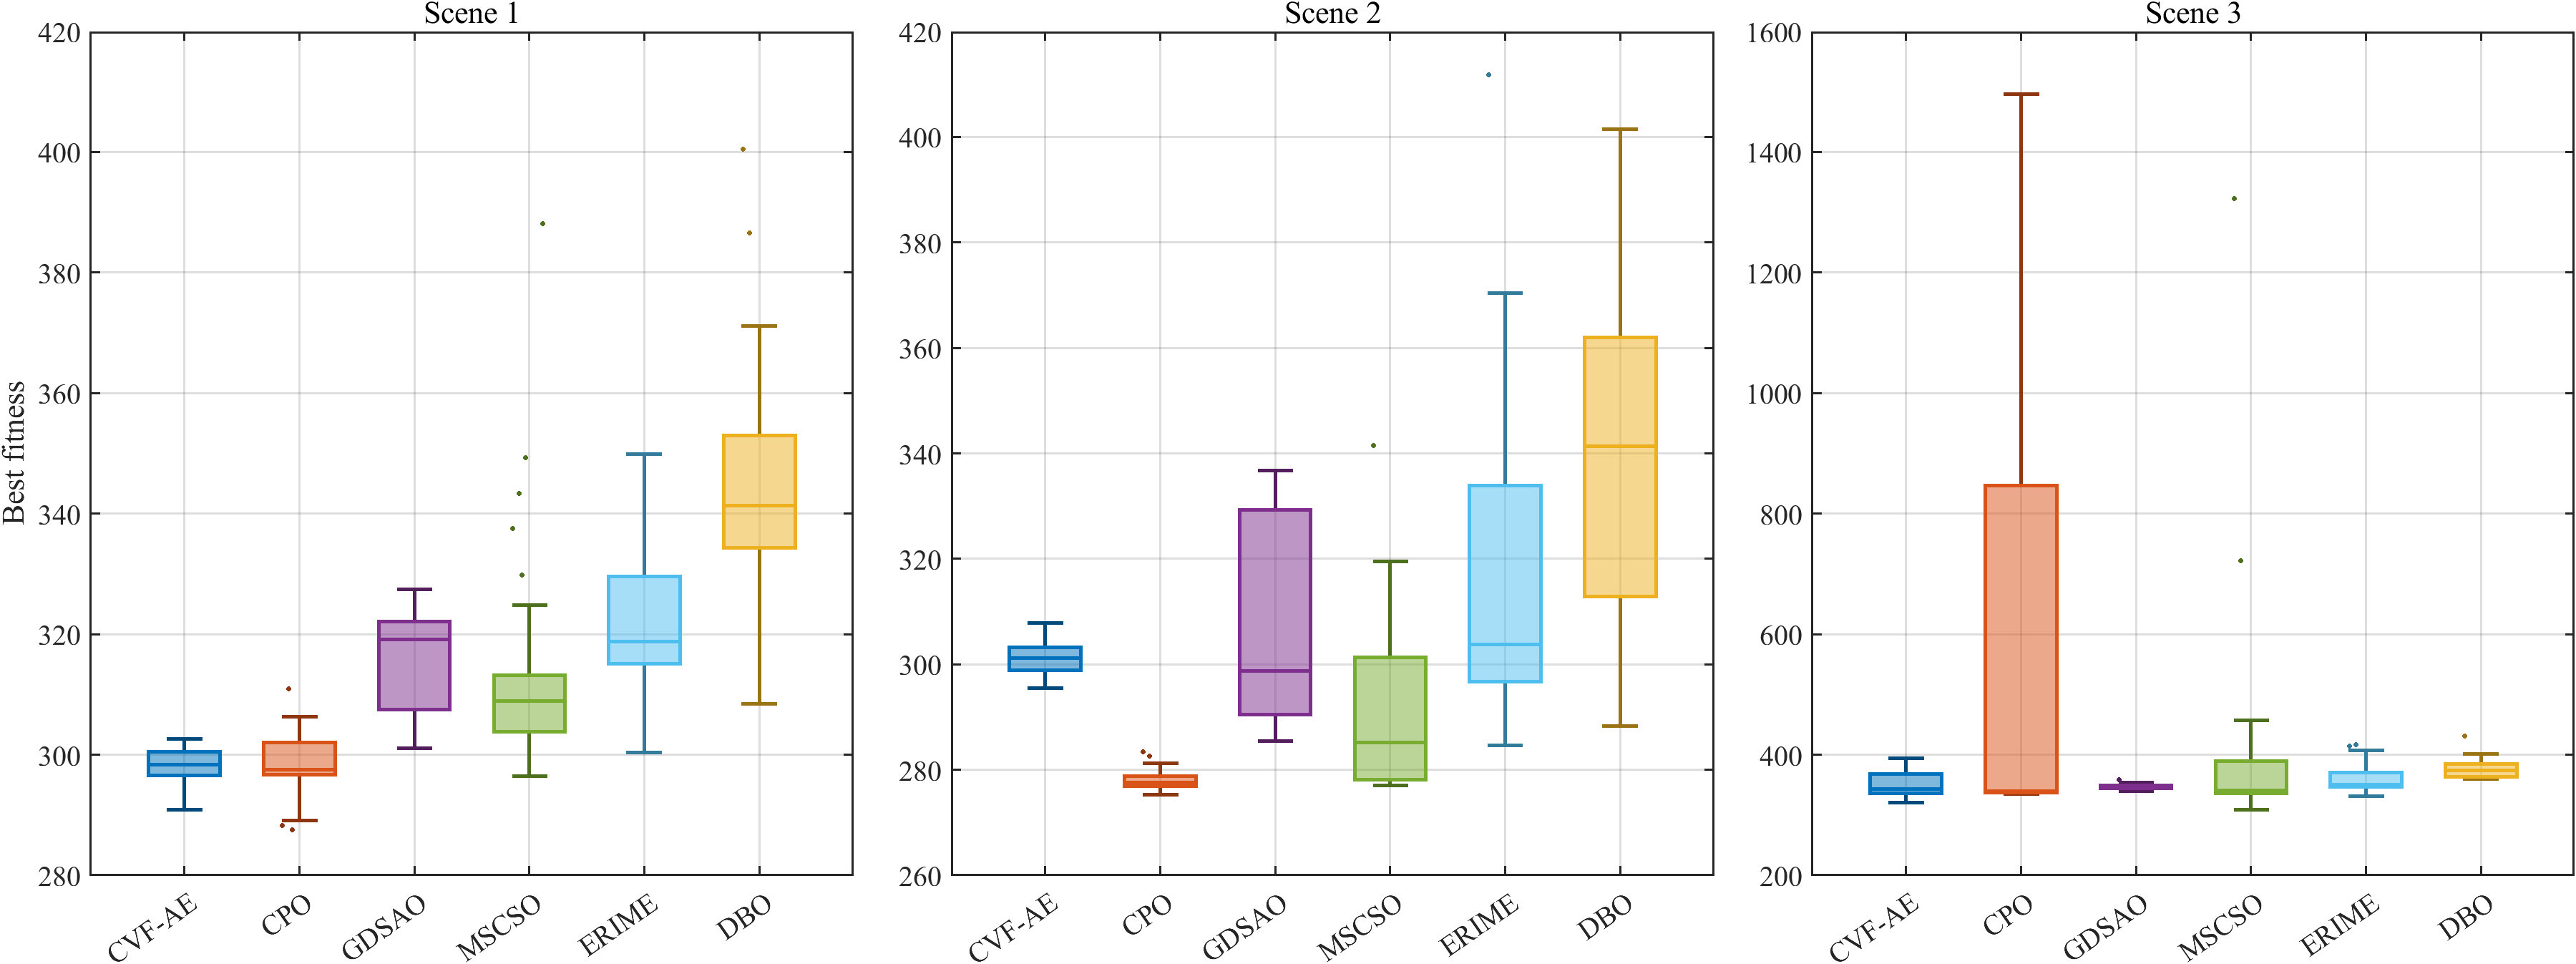
\includegraphics[width=\linewidth]{cvf_ae_boxplots_strong_algorithms.png}
\caption{强竞争算法的最终适应度分布}
\label{fig:boxplots-strong}
\end{figure}

图 \ref{fig:boxplots-strong} 展示了 CVF-AE 与强竞争算法的逐次运行分布。CVF-AE 在 Scene 1 和 Scene 3 中保持较低且较稳定的适应度分布；Scene 2 中 CPO 和 MSCSO 的箱体位置更低，对应表 \ref{tab:significance} 中的显著劣势，需要结合轨迹复核进一步解释。

在 Scene 1 中，CVF-AE 的平均适应度为 $298.1379$，略低于 CPO 的 $298.3594$，二者均达到 $1.00$ 的可行率。该场景相对宽松，强约束引导的优势主要体现在保持低风险、低绕行和稳定可行性，而不是拉开大幅标量差距。AE、WOA、HHO 和 PSO 在该场景中均出现较明显的可行率下降或适应度劣化，说明单纯基础进化搜索或无约束场机制难以稳定处理三维障碍、禁飞区和高度限制的组合。

在 Scene 2 中，CPO 和 MSCSO 的标量适应度分别为 $278.1196$ 和 $291.1680$，低于 CVF-AE 的 $301.2018$。因此，不能将 CVF-AE 写成该场景的标量最优方法。然而，轨迹复核显示 CPO 在该场景的高空复核标记率为 $1.00$，MSCSO 的高空复核标记率为 $0.50$，而 CVF-AE 的高空和边界复核标记率均为 $0$。这说明，较低的 scalar fitness 可能来自更激进的高度或通道选择，未必代表更符合低空走廊任务的路径。CVF-AE 在该场景提供的是更保守且稳定的可行路径，而不是单纯追求最低目标值。

在 Scene 3 中，GDSAO 的平均适应度为 $346.8474$，略低于 CVF-AE 的 $349.2270$；但 GDSAO 的边界贴靠复核标记率达到 $0.9667$，ERIME 也达到 $0.9667$，DBO 为 $0.9000$。相比之下，CVF-AE 的 Scene 3 边界贴靠复核标记率为 $0.1667$，且可行率保持 $1.00$。因此，Scene 3 的结果进一步表明，强约束低空路径规划不能只依据最终适应度排序，还需要检查路径是否过度贴近空间边界、是否绕开了实际低空走廊以及是否保持可行。

图 \ref{fig:convergence} 给出了三类场景的收敛行为。CVF-AE 在 Scene 1 和 Scene 3 中能够较快进入稳定低适应度区间；Scene 2 中 CPO 的最终均值更低，进一步说明本文结论应聚焦综合工程表现，而不是单一收敛终值。

\begin{figure}[tbp]
\centering
\begin{subfigure}{0.96\linewidth}
    \centering
    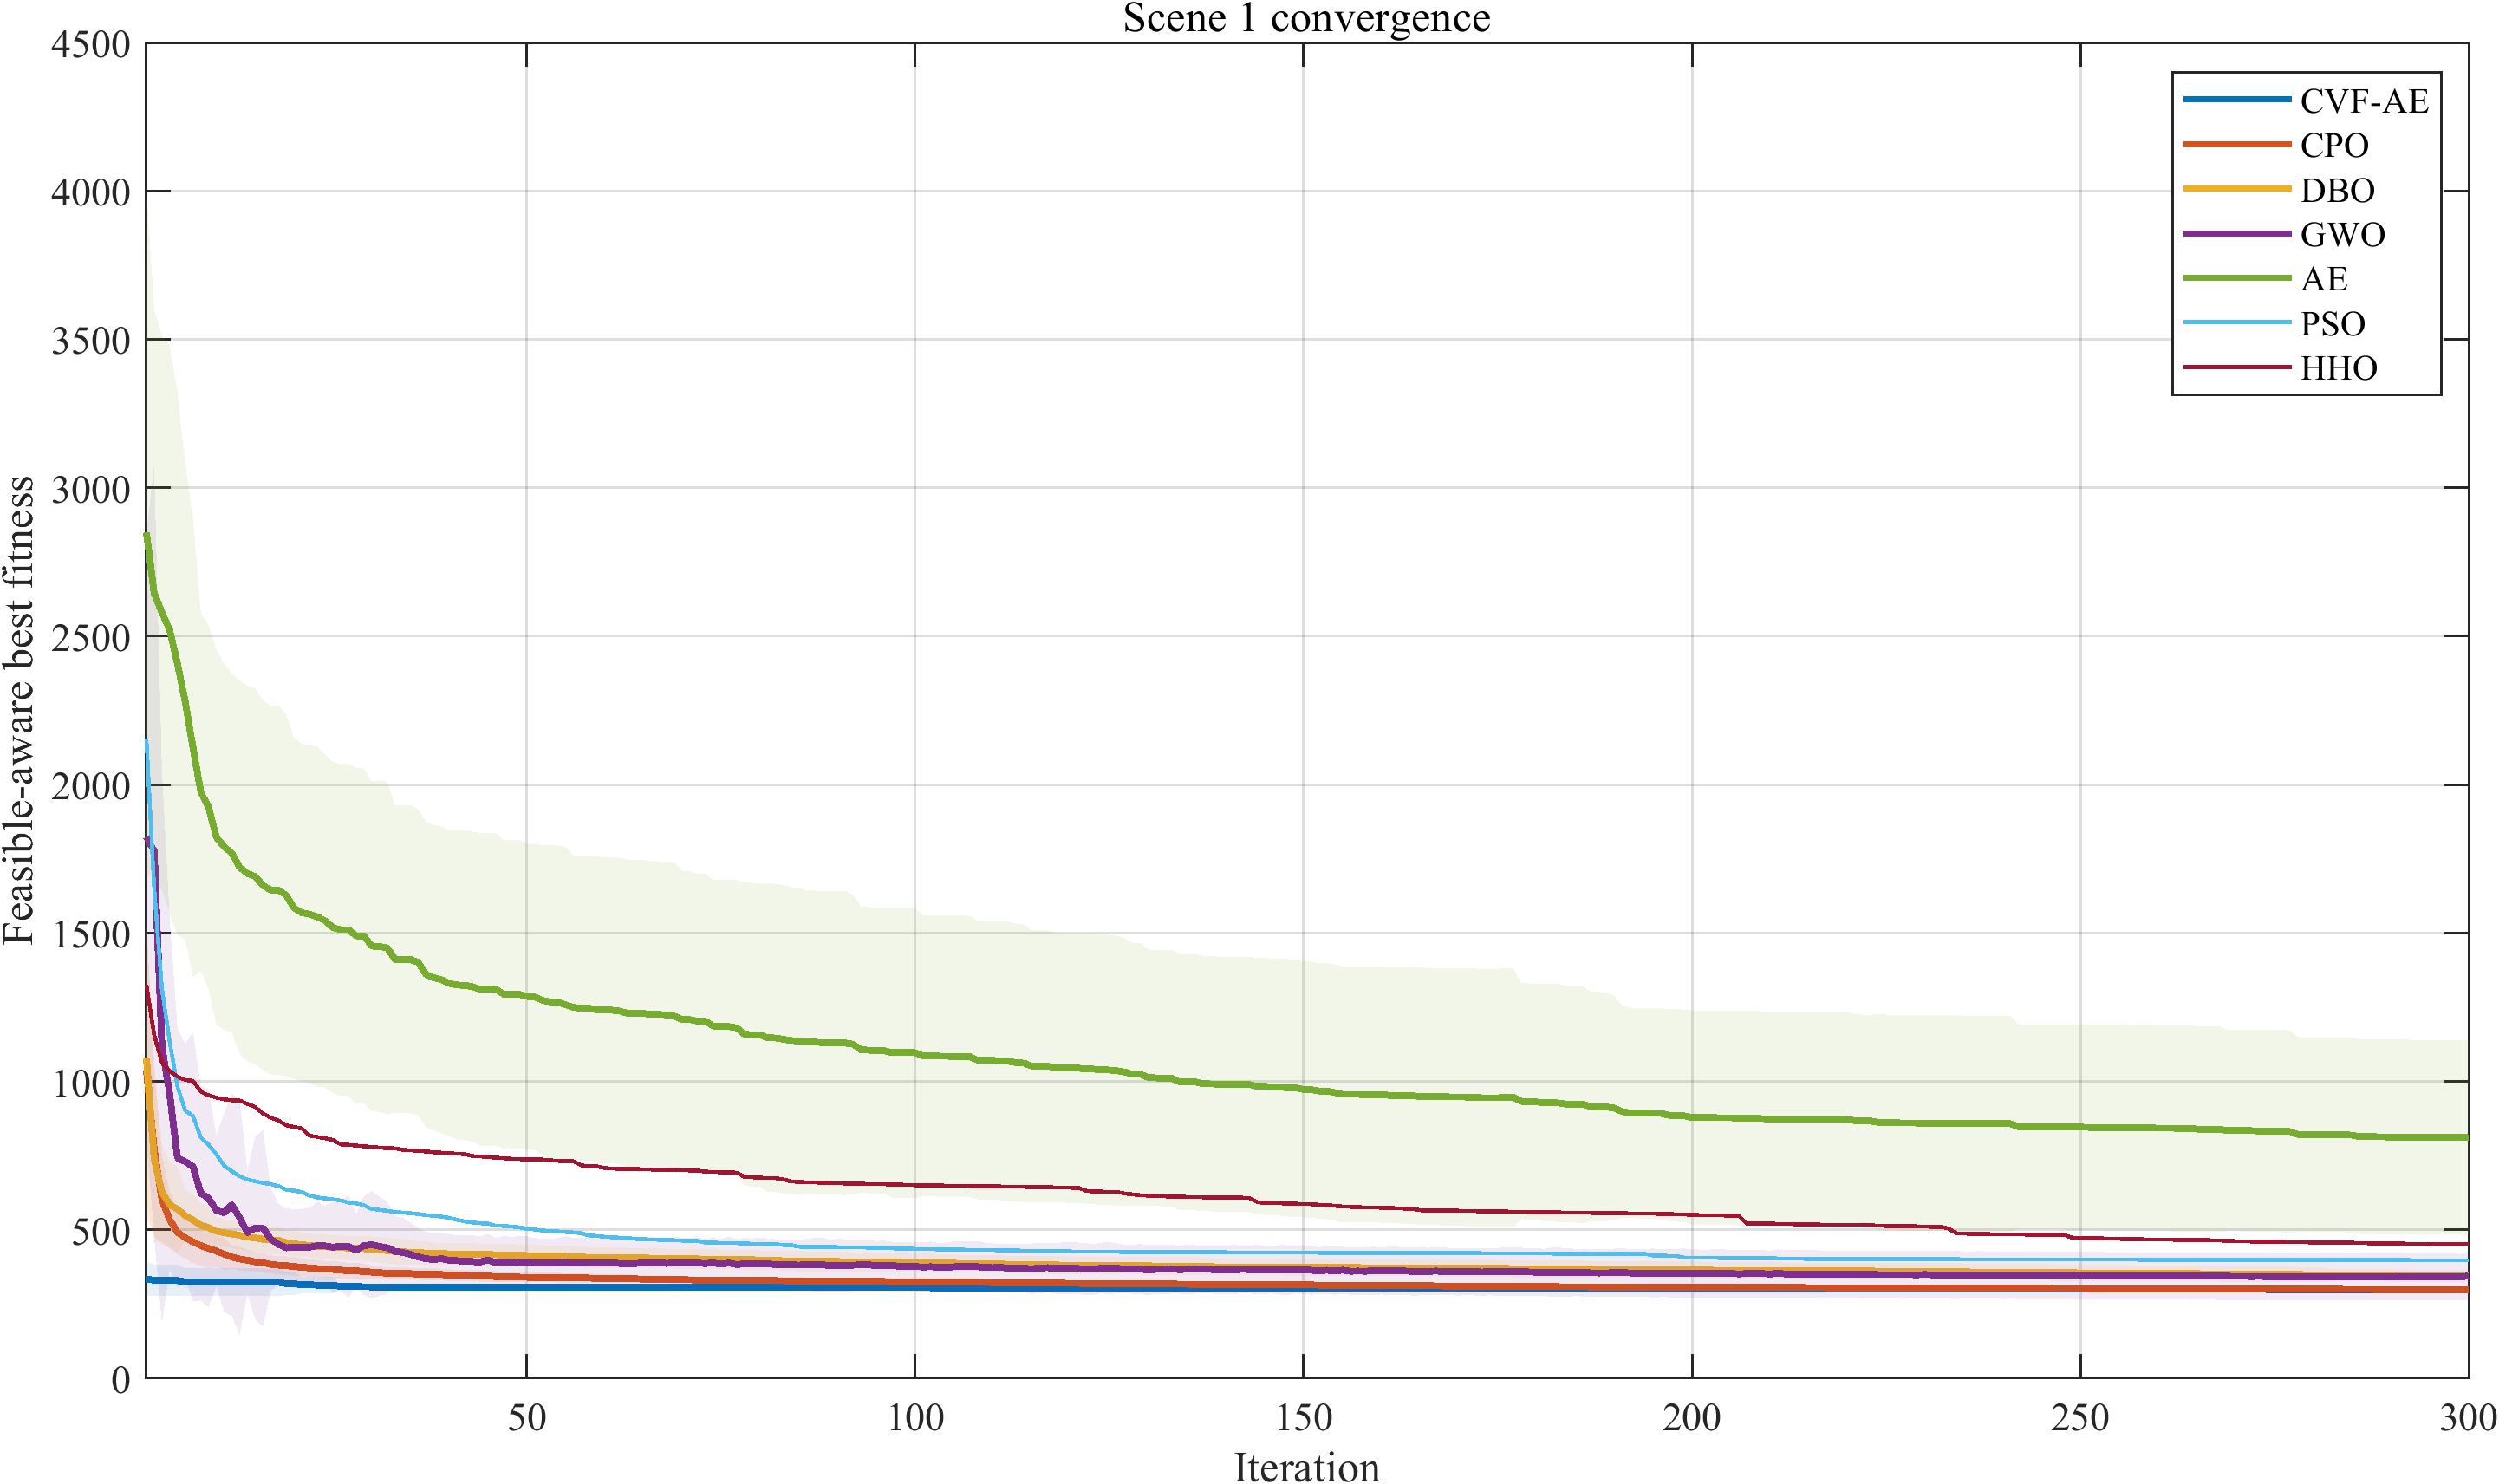
\includegraphics[width=\linewidth]{scene1_convergence_mean_std.png}
    \caption{Scene 1}
\end{subfigure}

\begin{subfigure}{0.96\linewidth}
    \centering
    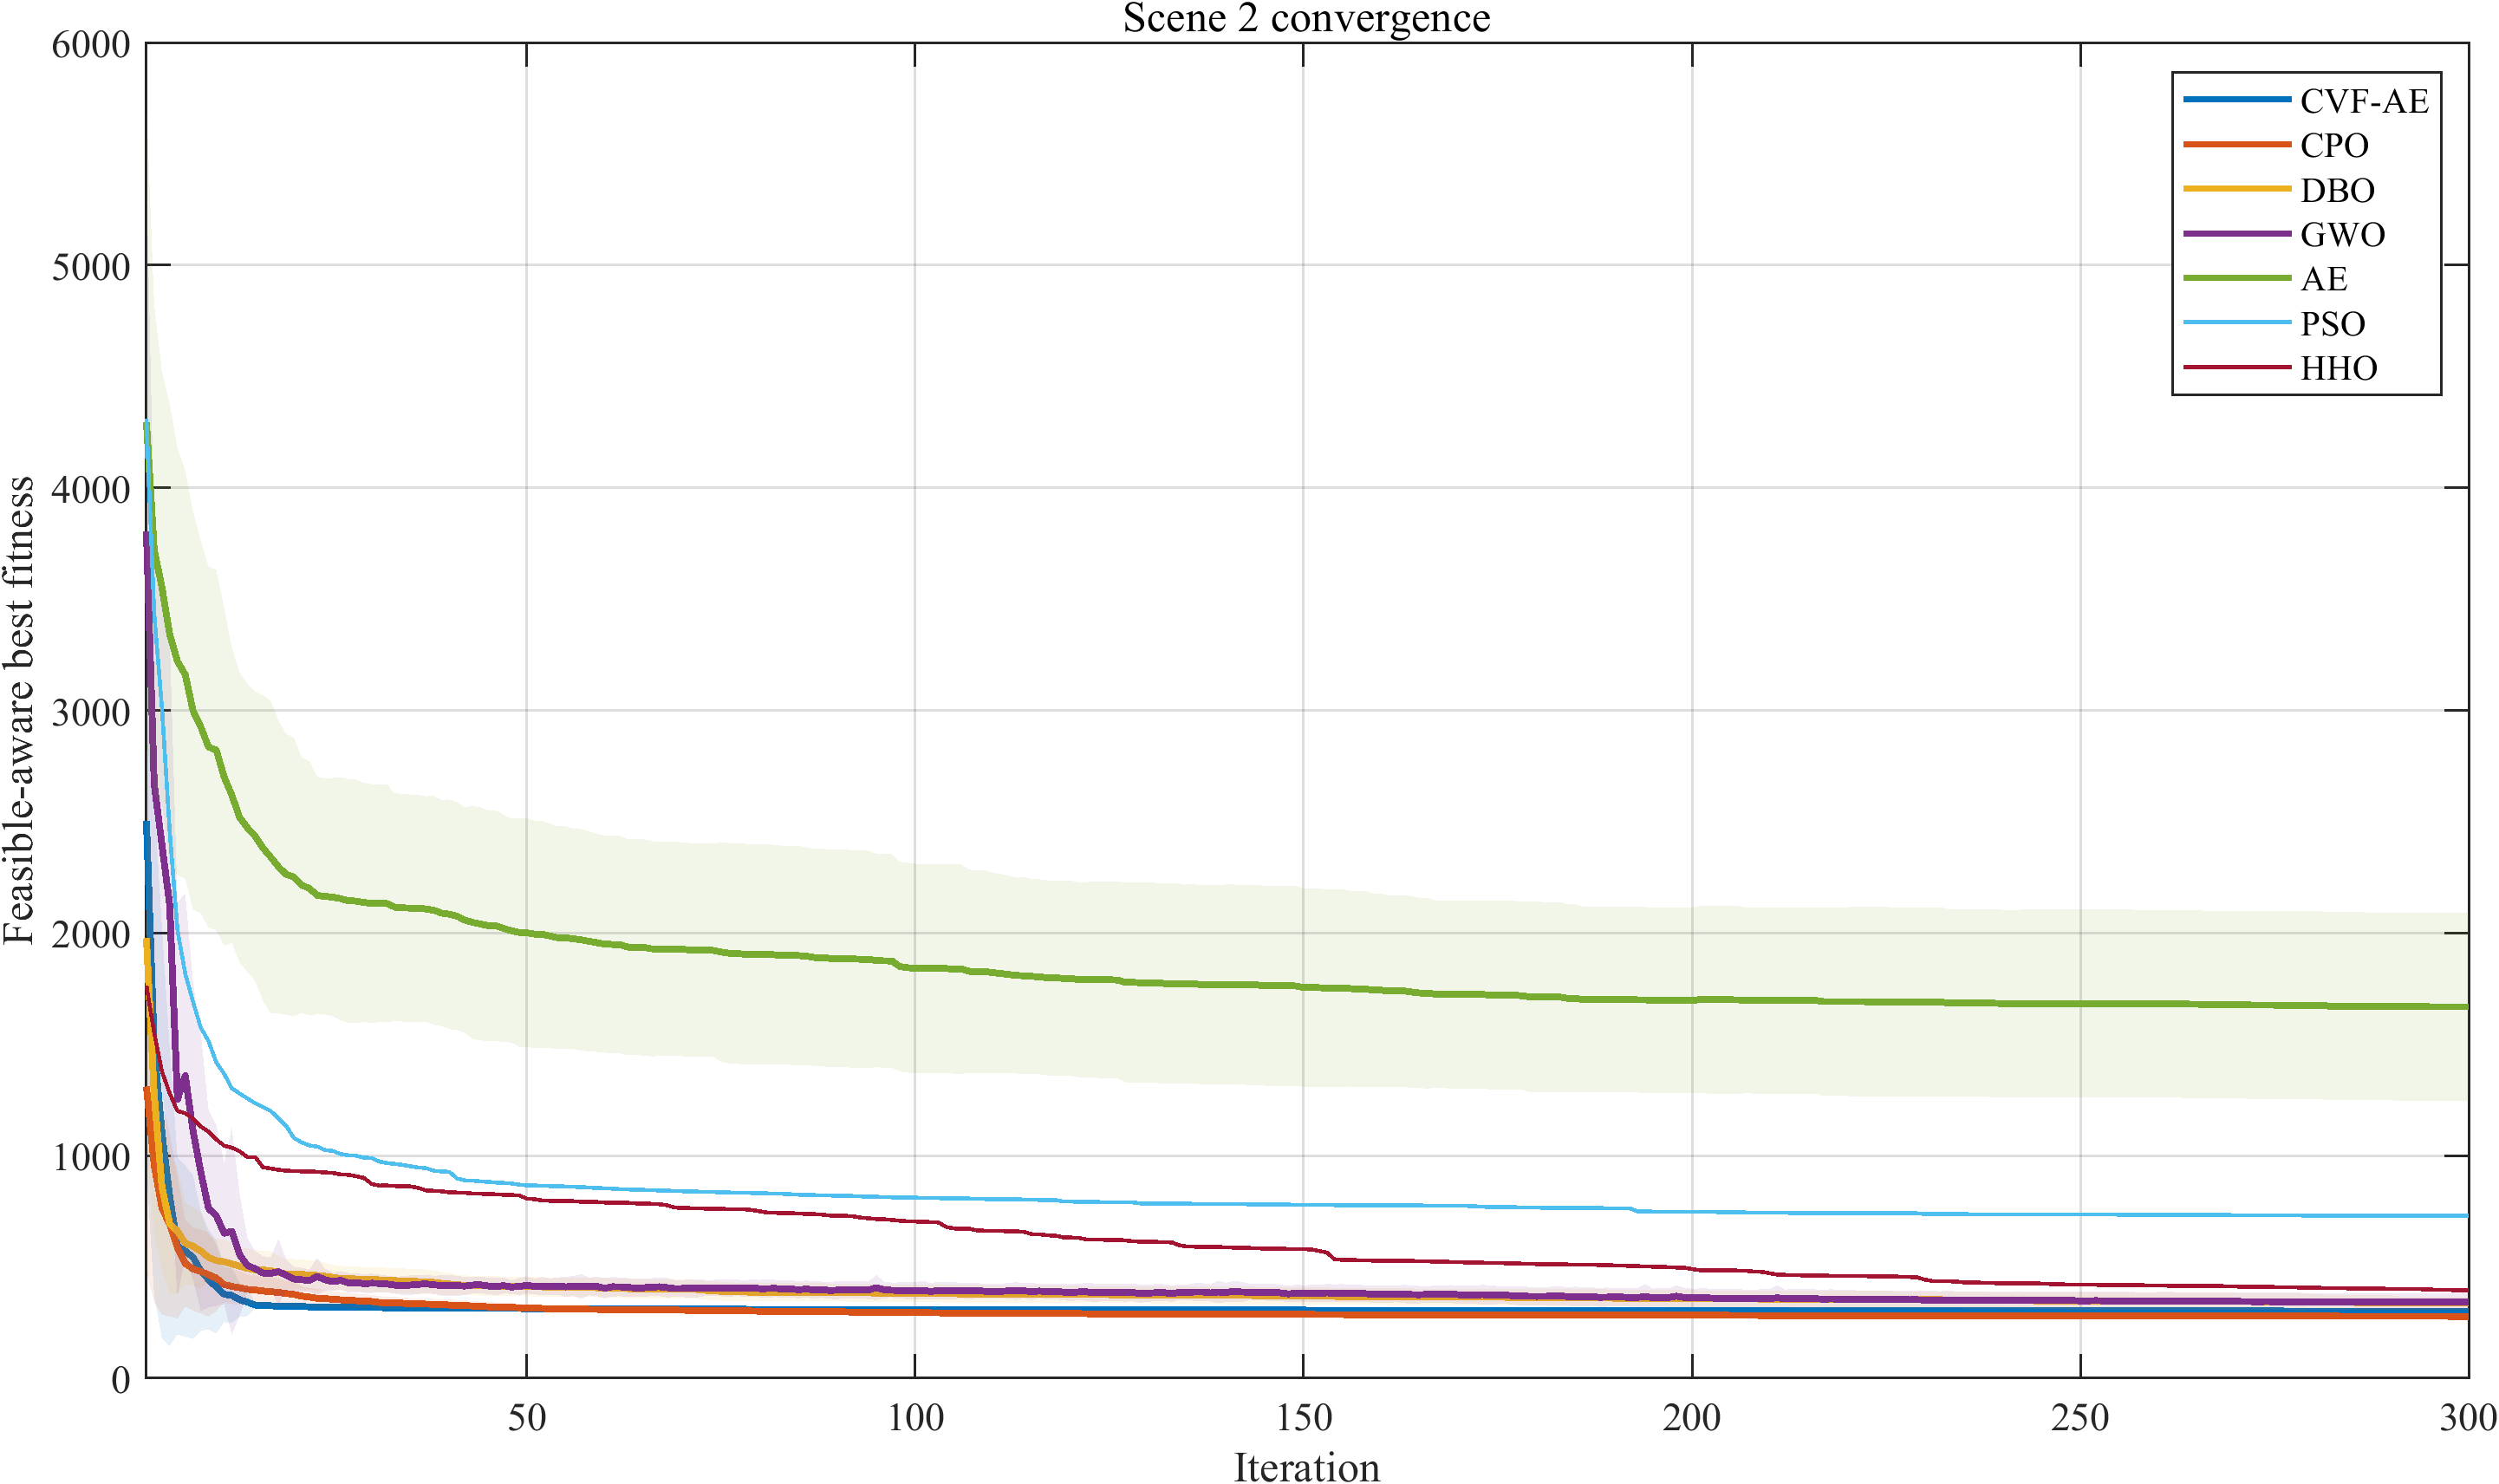
\includegraphics[width=\linewidth]{scene2_convergence_mean_std.png}
    \caption{Scene 2}
\end{subfigure}

\begin{subfigure}{0.96\linewidth}
    \centering
    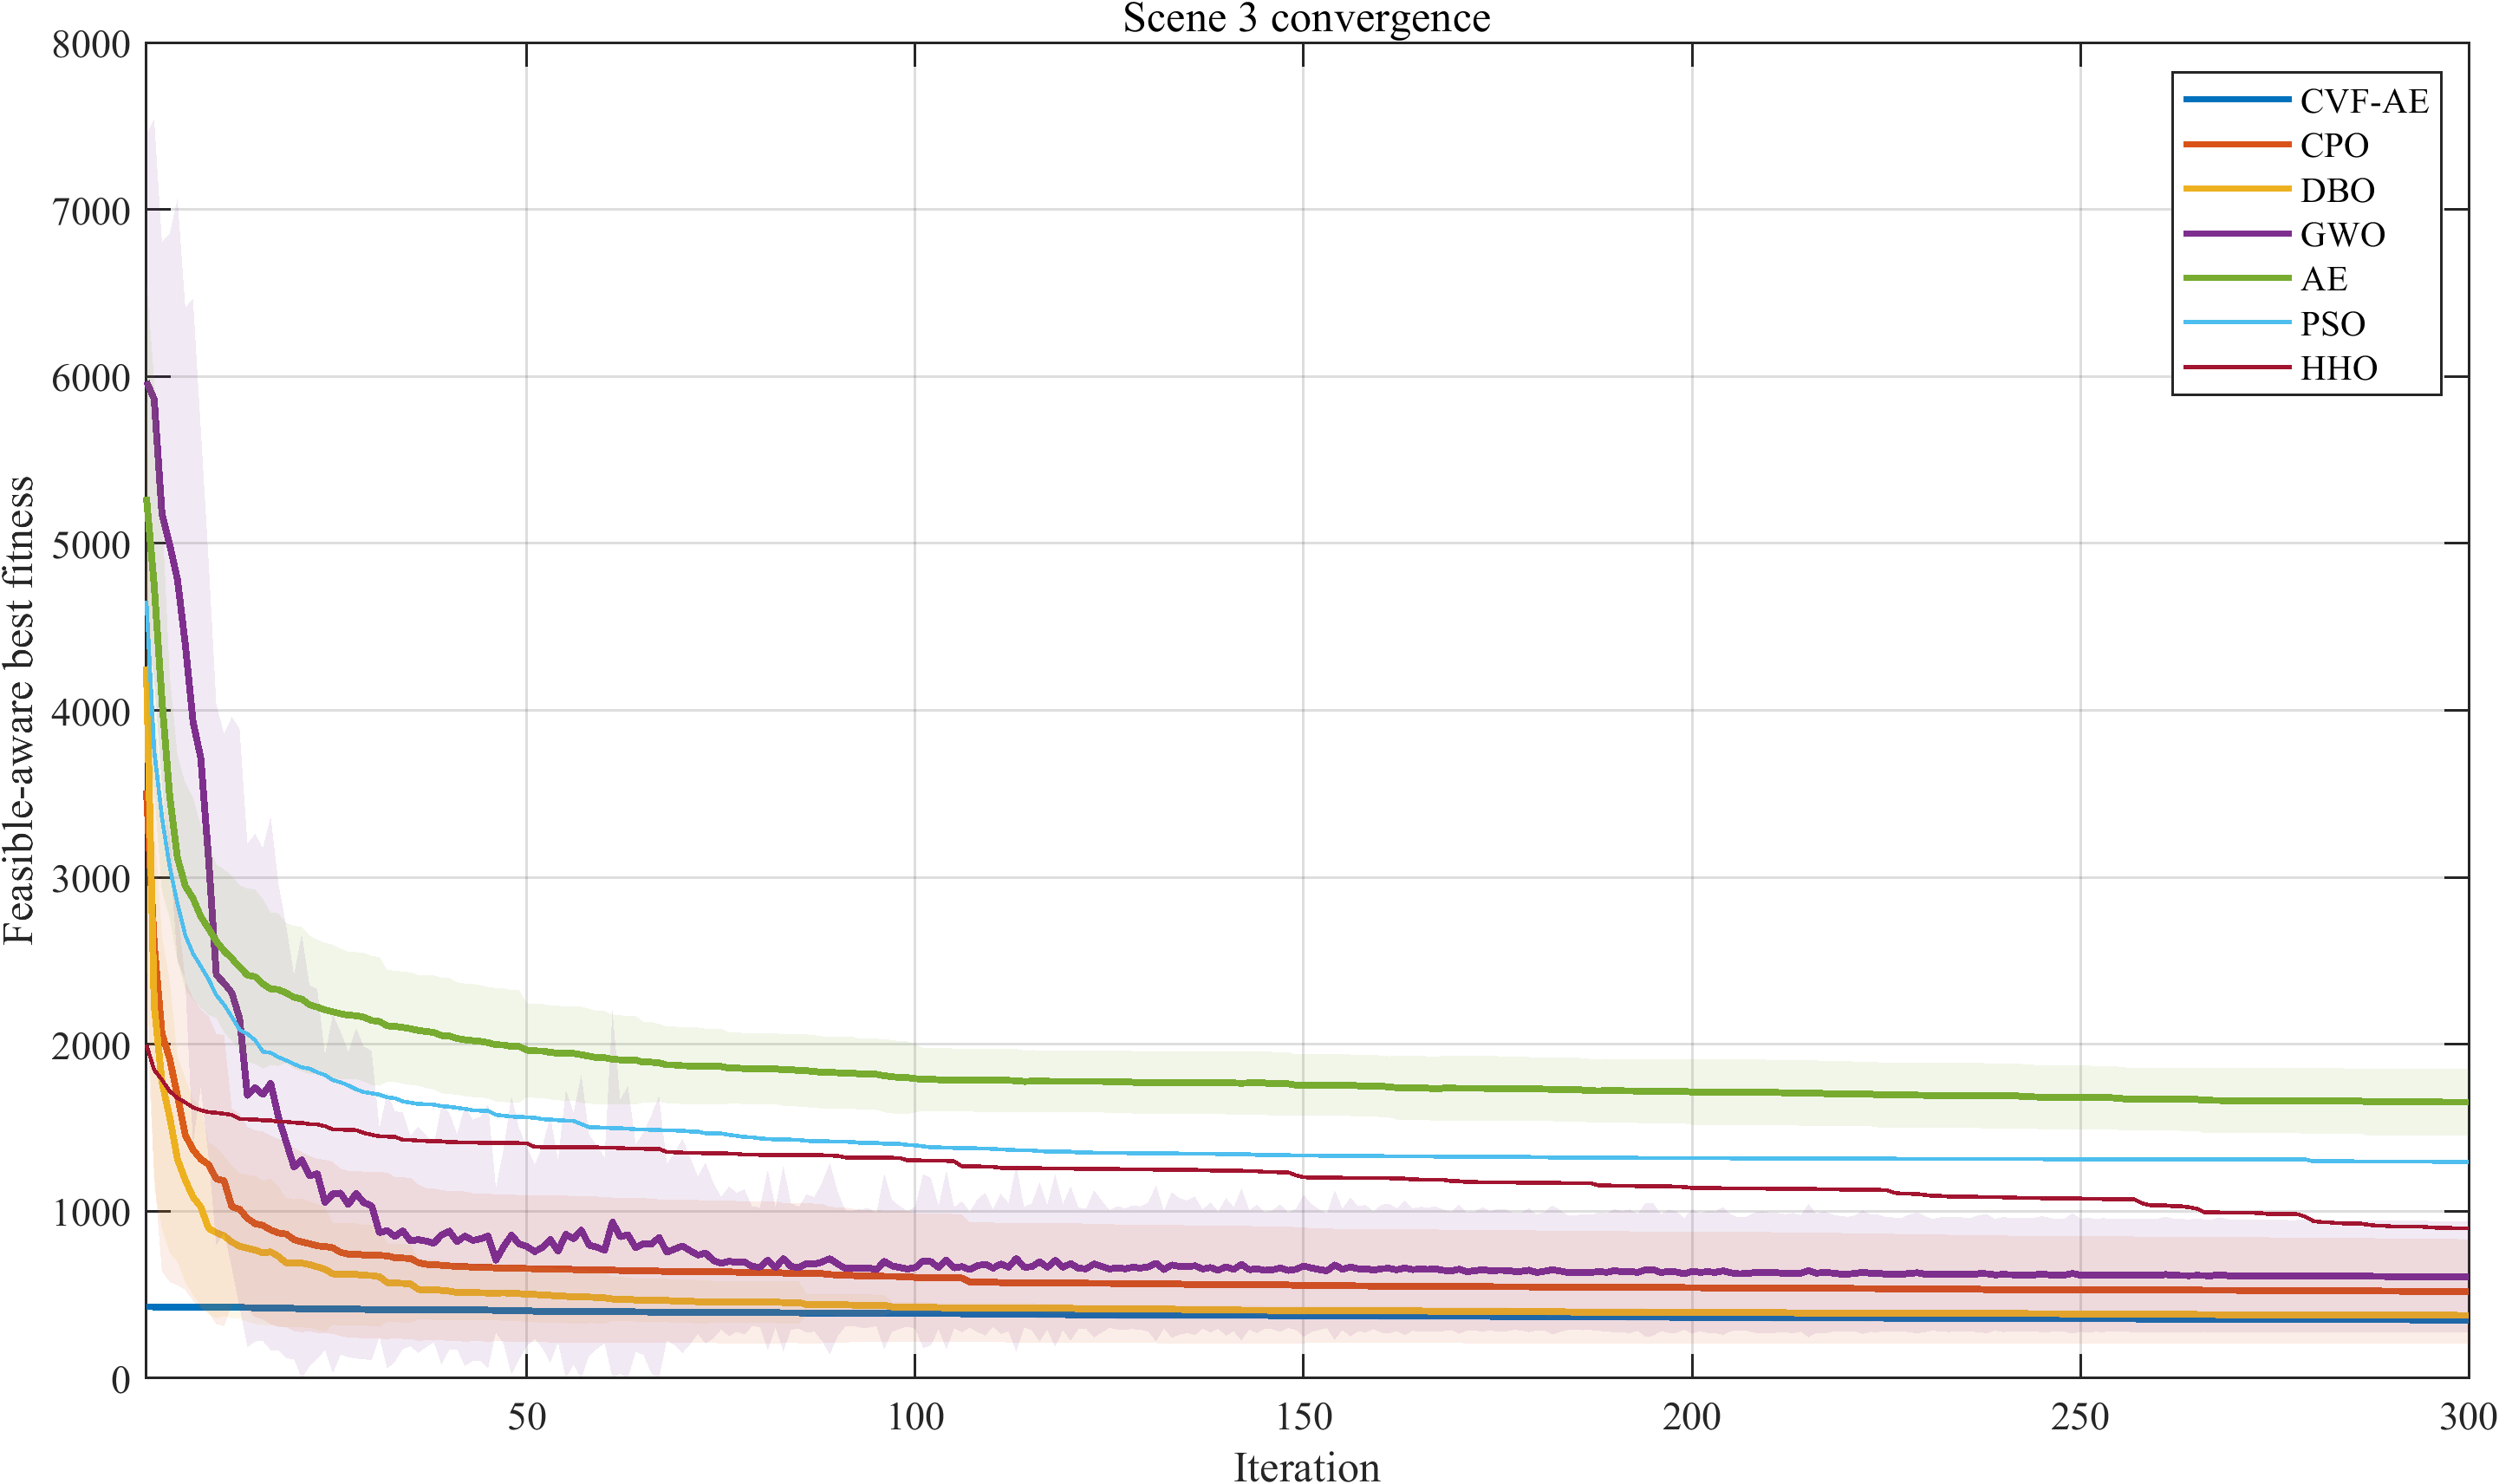
\includegraphics[width=\linewidth]{scene3_convergence_mean_std.png}
    \caption{Scene 3}
\end{subfigure}
\caption{三类测试场景的平均收敛曲线}
\label{fig:convergence}
\end{figure}

图 \ref{fig:extended-paths-top} 和图 \ref{fig:extended-paths-3d} 分别从俯视视角和三维视角展示轨迹层面的差异。三维视图用于观察高度变化和障碍物空间关系，俯视轨迹更容易暴露边界贴靠、过度绕行和局部通道选择问题。与只看适应度均值相比，两类视图共同说明了本文在 Scene 2 和 Scene 3 中对 CPO、GDSAO、ERIME 与 MSCSO 保持谨慎解释的原因。

\subsection{统计显著性分析}

\begin{table}[tbp]
\centering
\caption{CVF-AE 与基线算法的逐场景显著性比较}
\label{tab:significance}
\scriptsize
\setlength{\tabcolsep}{2.8pt}
\begin{tabular}{@{}llccc@{}}
\toprule
Baseline & Scene & $p_{\mathrm{Holm}}$ & $\delta$ & R \\
\midrule
AE & 1 & 3.0e-10 & +1.00 & + \\
AE & 2 & 3.0e-10 & +1.00 & + \\
AE & 3 & 3.0e-10 & +1.00 & + \\
PSO & 1 & 2.0e-07 & +0.81 & + \\
PSO & 2 & 5.5e-04 & +0.59 & + \\
PSO & 3 & 3.0e-10 & +1.00 & + \\
GWO & 1 & 3.0e-10 & +1.00 & + \\
GWO & 2 & 0.001 & +0.55 & + \\
GWO & 3 & 2.1e-05 & +0.70 & + \\
WOA & 1 & 3.0e-10 & +1.00 & + \\
WOA & 2 & 3.0e-10 & +1.00 & + \\
WOA & 3 & 3.0e-10 & +1.00 & + \\
HHO & 1 & 1.0e-09 & +0.95 & + \\
HHO & 2 & 0.001 & +0.55 & + \\
HHO & 3 & 5.9e-08 & +0.87 & + \\
DBO & 1 & 3.0e-10 & +1.00 & + \\
DBO & 2 & 1.5e-06 & +0.78 & + \\
DBO & 3 & 5.1e-05 & +0.66 & + \\
CPO & 1 & 0.773 & +0.04 & = \\
CPO & 2 & 3.0e-10 & -1.00 & - \\
CPO & 3 & 0.934 & +0.14 & = \\
GDSAO & 1 & 5.5e-10 & +0.97 & + \\
GDSAO & 2 & 0.620 & -0.08 & = \\
GDSAO & 3 & 0.934 & +0.15 & = \\
ERIME & 1 & 4.0e-10 & +0.98 & + \\
ERIME & 2 & 0.595 & +0.16 & = \\
ERIME & 3 & 0.097 & +0.34 & = \\
MSCSO & 1 & 4.8e-07 & +0.78 & + \\
MSCSO & 2 & 0.002 & -0.51 & - \\
MSCSO & 3 & 0.934 & +0.13 & = \\
\bottomrule
\end{tabular}
\end{table}


表 \ref{tab:significance} 给出了主对比中 CVF-AE 与每个基线的逐场景 Holm 校正 $p$ 值和 Cliff's delta。三个场景的 Kruskal--Wallis 总体检验均显示算法间分布存在显著差异；进一步的成对比较采用双侧 Wilcoxon rank-sum 检验，并在每个场景内使用 Holm 校正。主对比中，CVF-AE 对 10 个基线算法的逐场景比较共得到 $21$ 胜、$7$ 平和 $2$ 负。两项显著劣势均出现在 Scene 2，分别对应 CPO 和 MSCSO 的标量适应度优势。表中 $R$ 表示 Holm 校正后的胜、平、负关系；$\delta$ 按最小化问题定义，正值表示 CVF-AE 的最终适应度分布更优，负值表示对应基线更优。

该统计结果支持两个结论。第一，CVF-AE 在多数场景和多数基线上具有显著或至少不劣的适应度表现，尤其相对于 AE、PSO、GWO、WOA、HHO 和 DBO 等基线表现稳定。第二，统计检验本身只作用于最终最佳适应度分布，不能替代轨迹合理性判断。Scene 2 中 CPO 和 MSCSO 的标量优势是真实存在的，但结合高空复核标记和 Scene 3 的可行率/边界贴靠风险后，本文更适合将 CVF-AE 的结论表述为综合均衡优势，而不是逐场景标量最优。

\begin{figure*}[tbp]
\centering
\begin{subfigure}{0.32\linewidth}
    \centering
    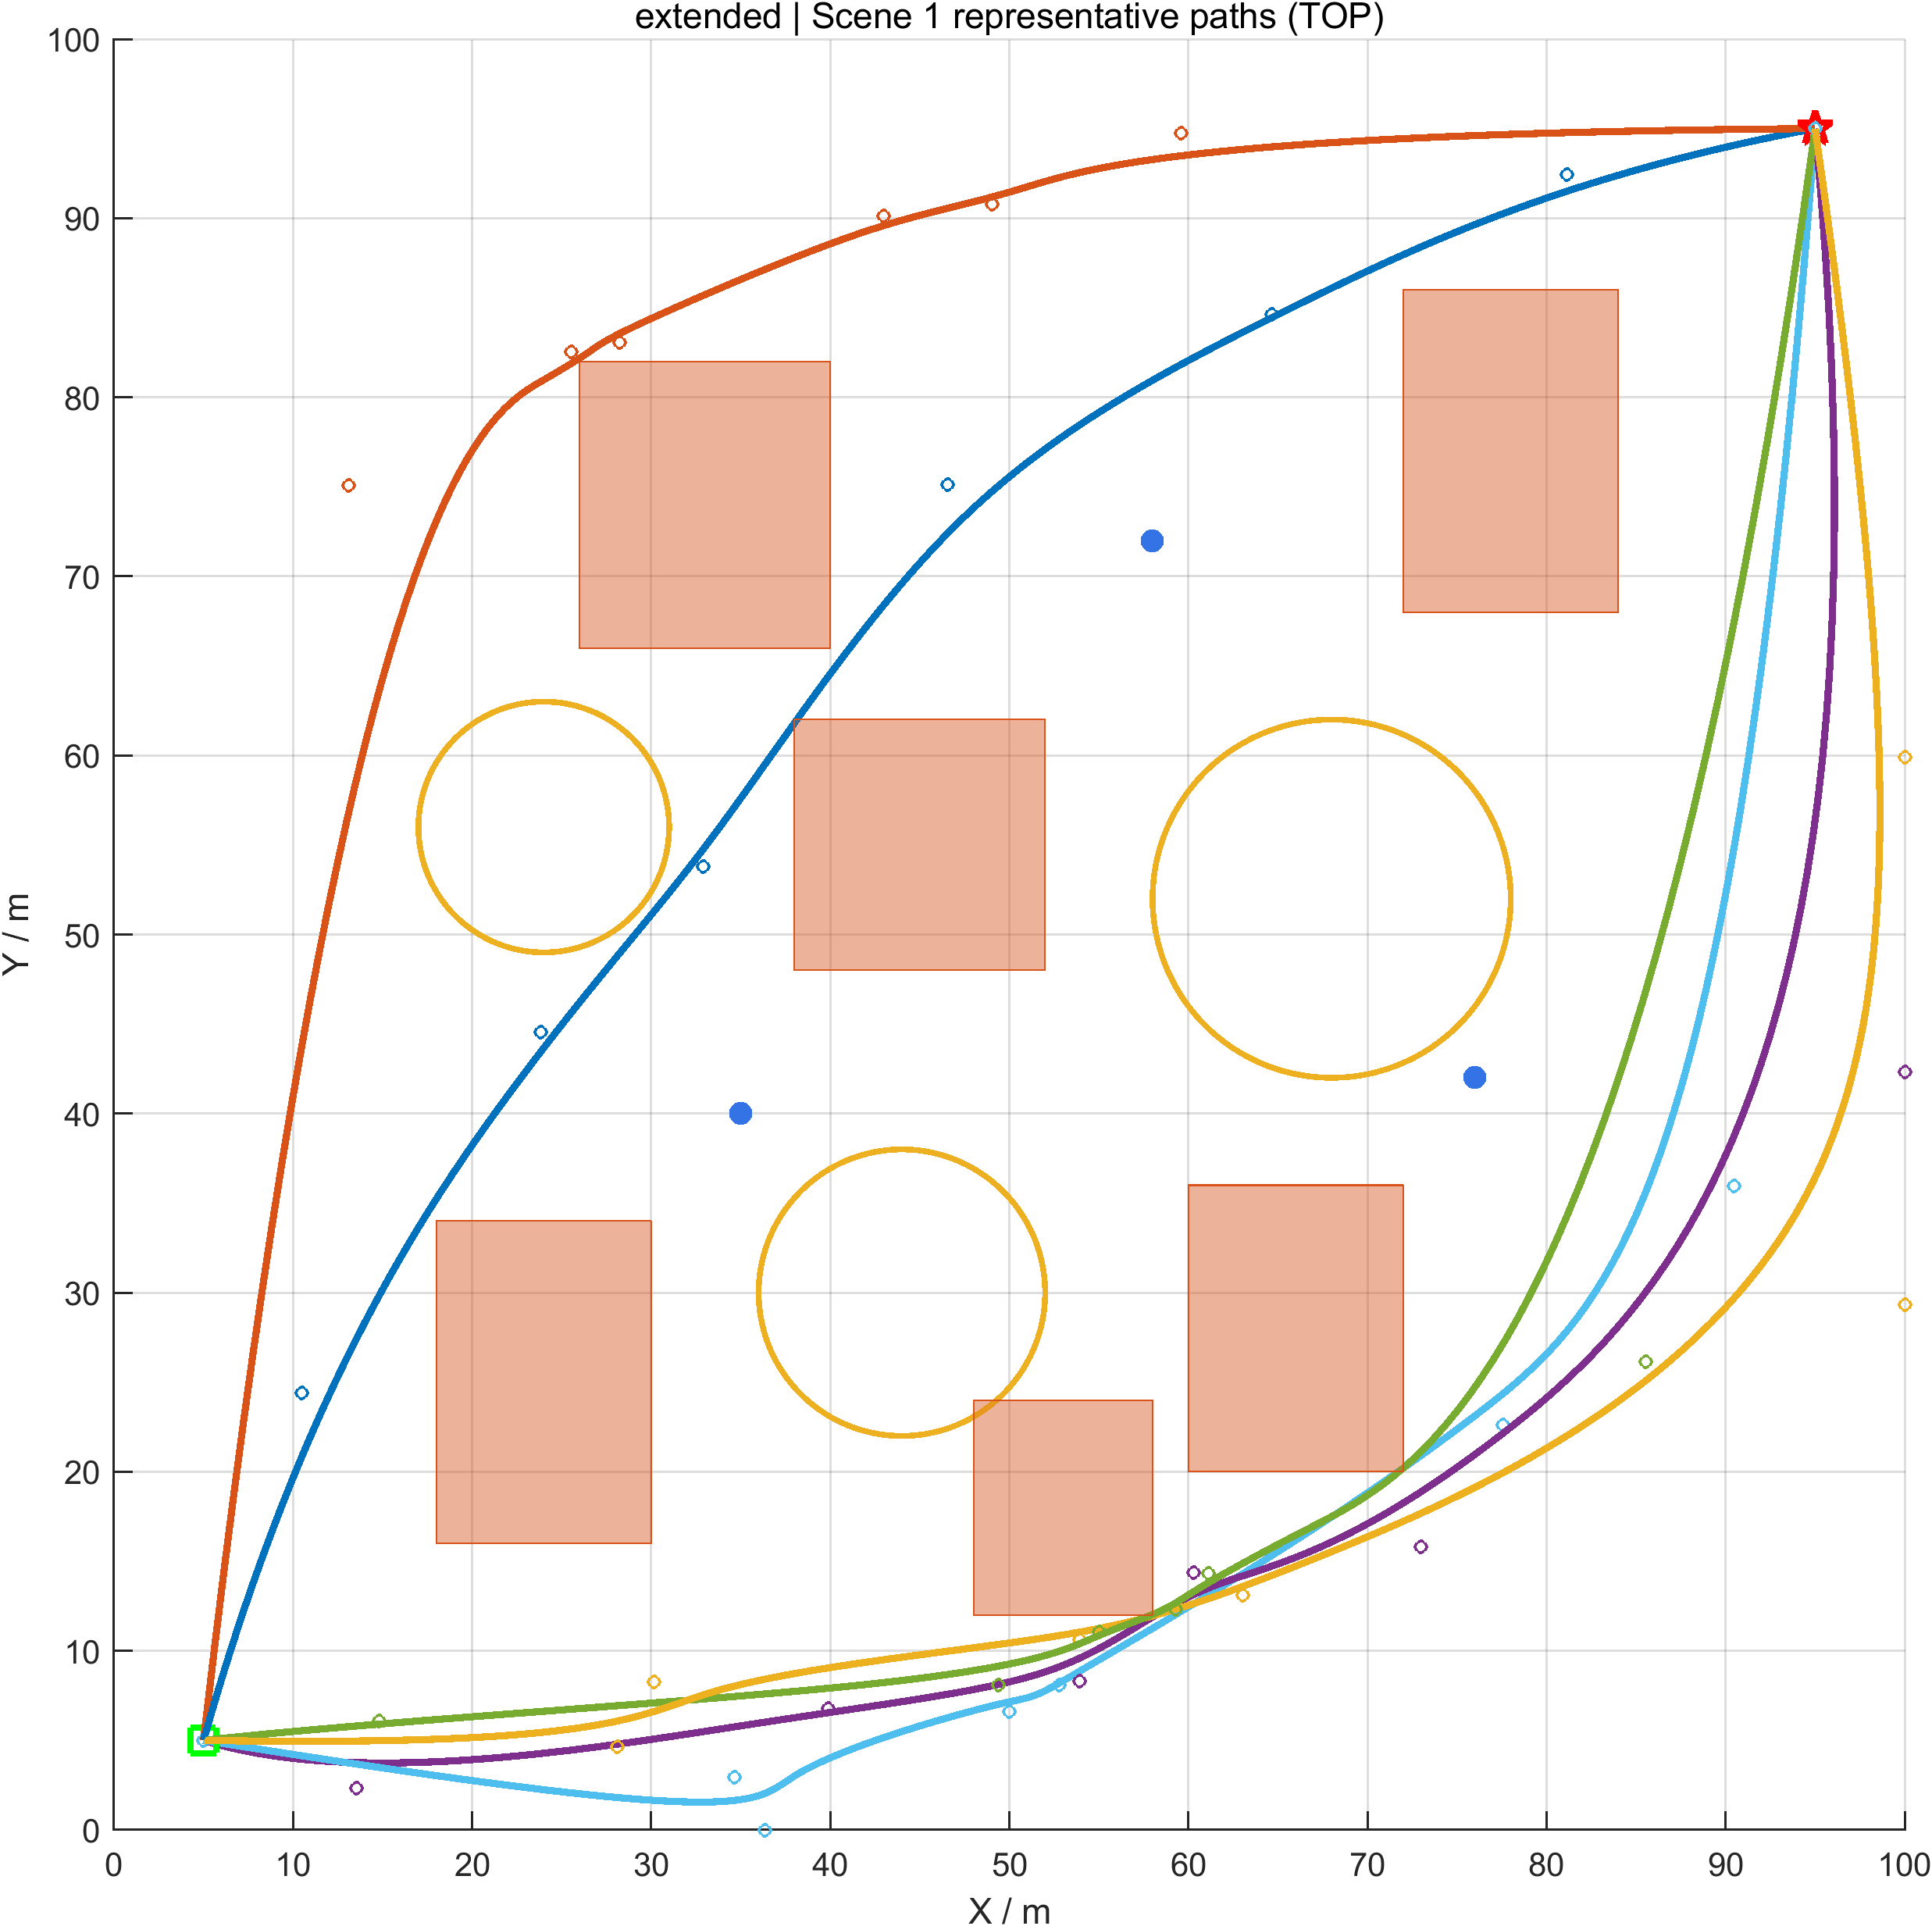
\includegraphics[width=\linewidth]{extended_scene1_representative_top.png}
    \caption{Scene 1}
\end{subfigure}
\hfill
\begin{subfigure}{0.32\linewidth}
    \centering
    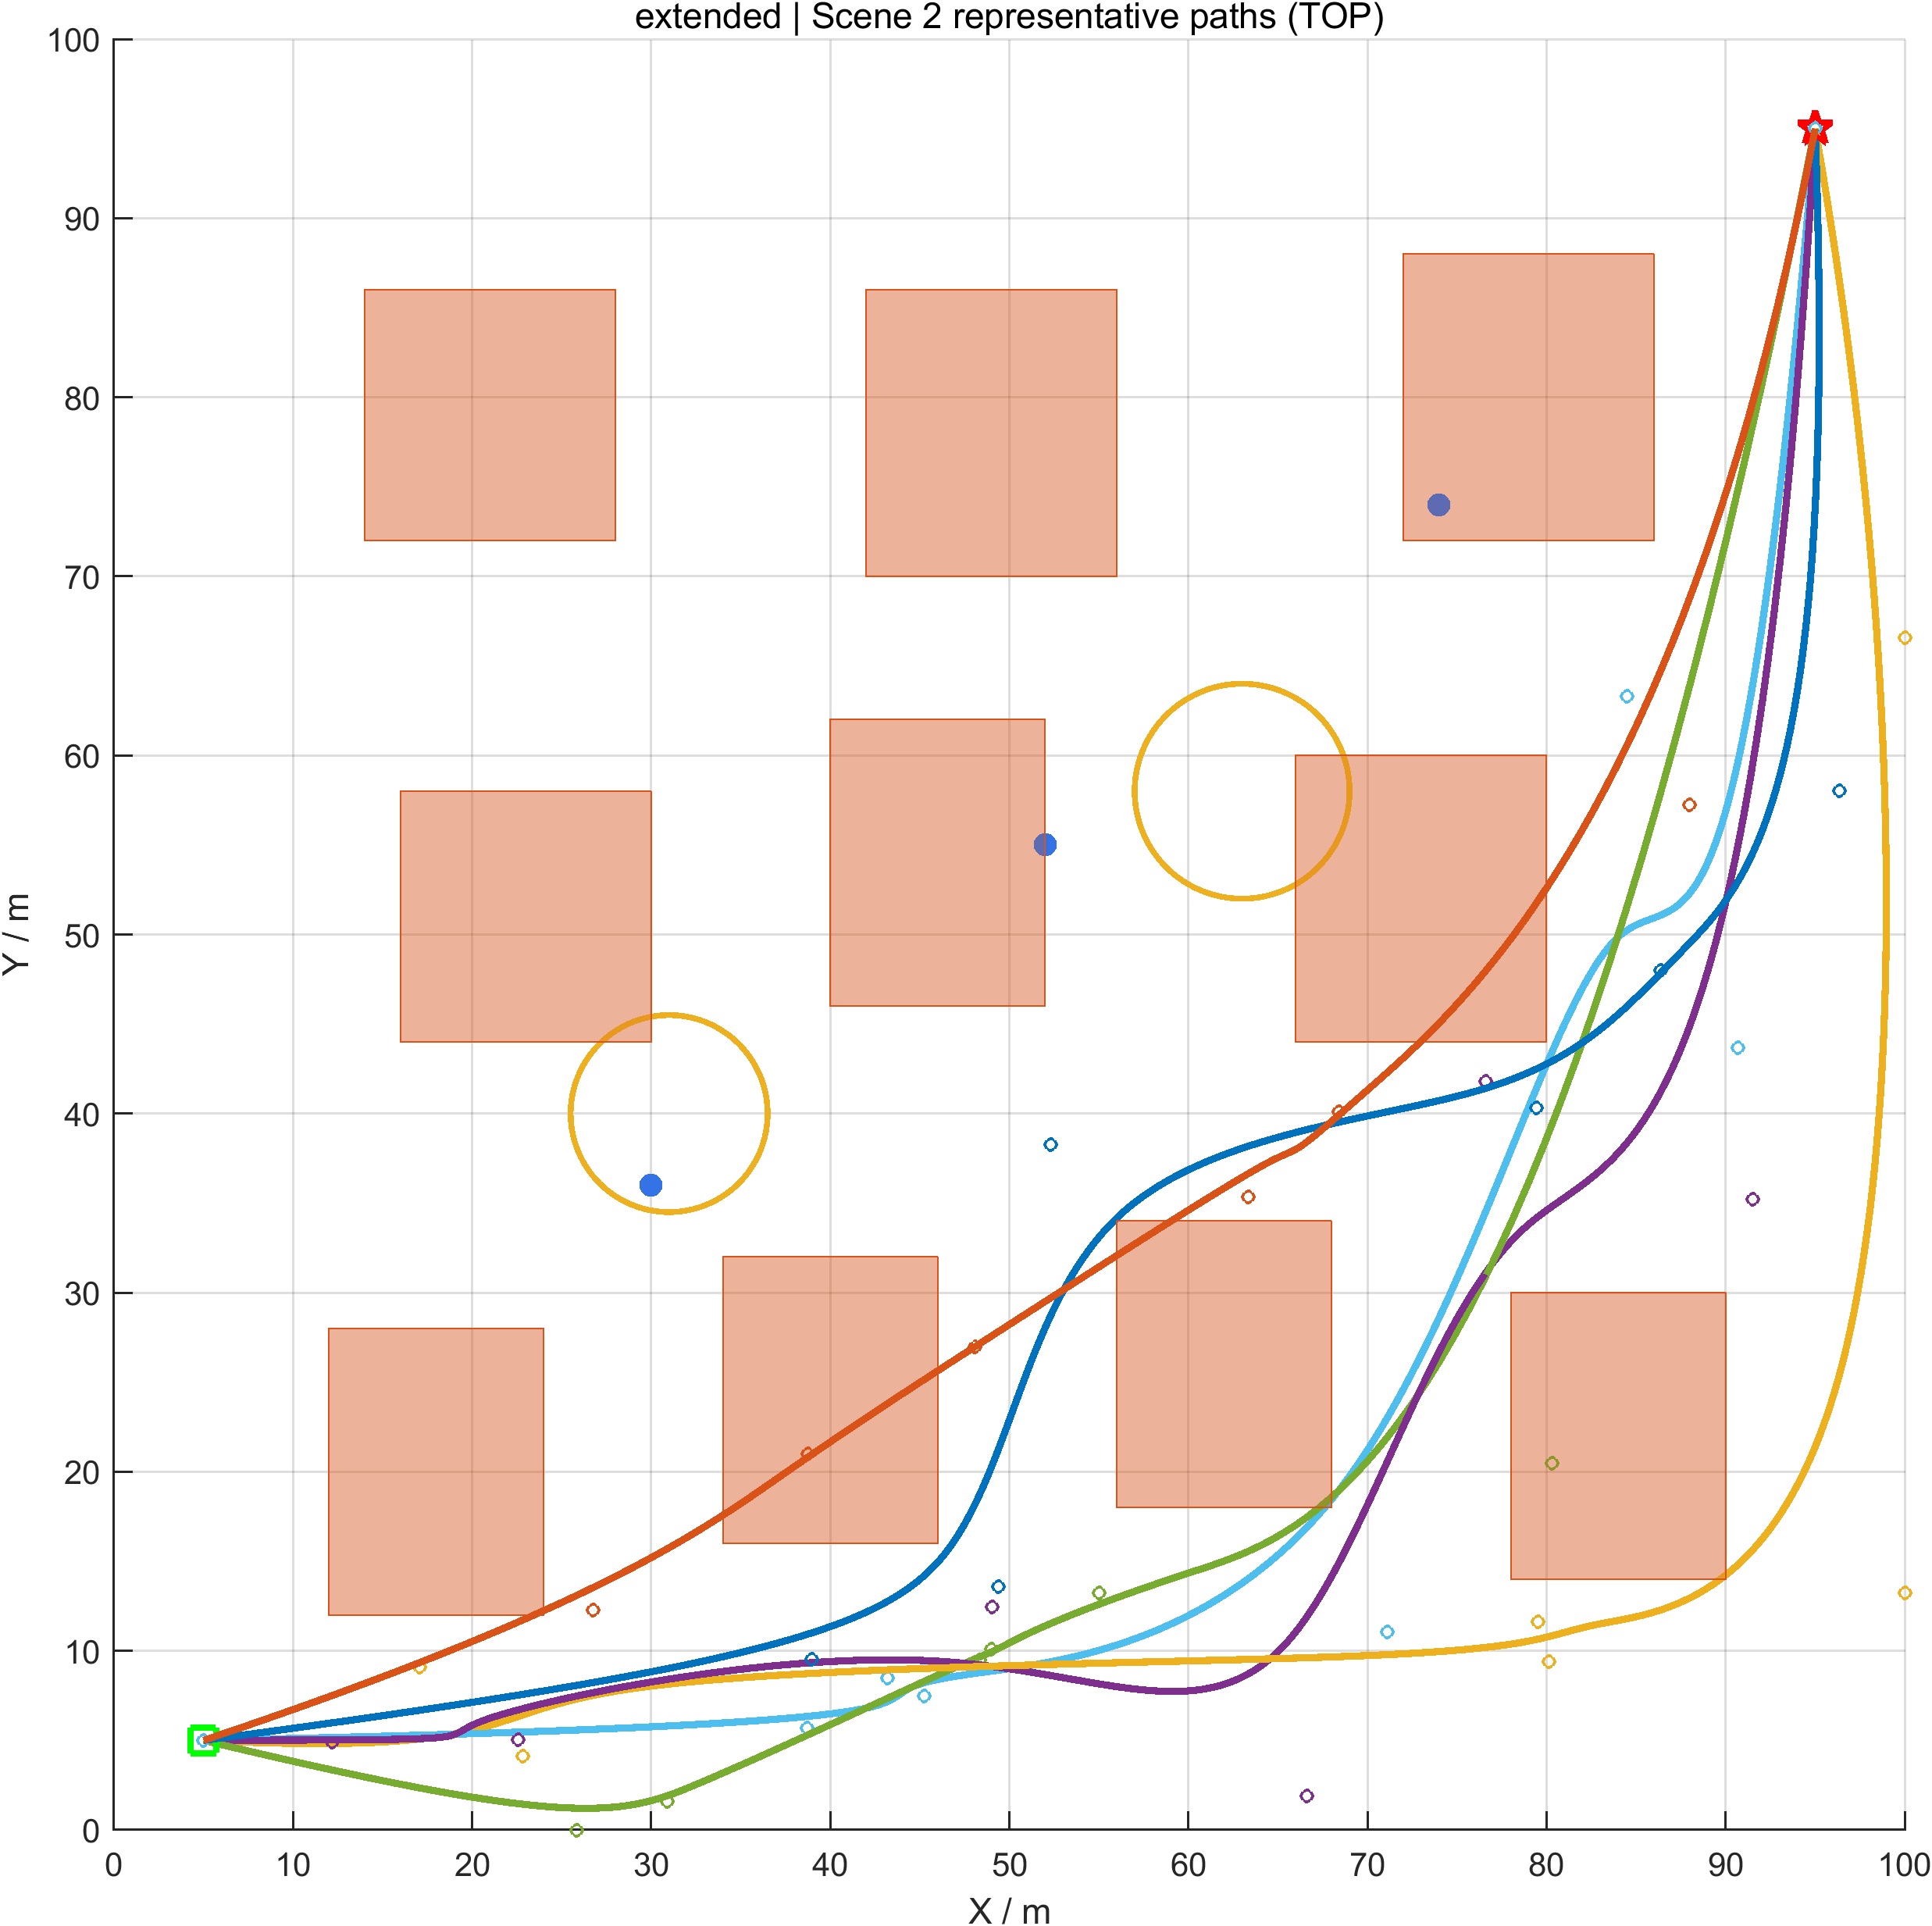
\includegraphics[width=\linewidth]{extended_scene2_representative_top.png}
    \caption{Scene 2}
\end{subfigure}
\hfill
\begin{subfigure}{0.32\linewidth}
    \centering
    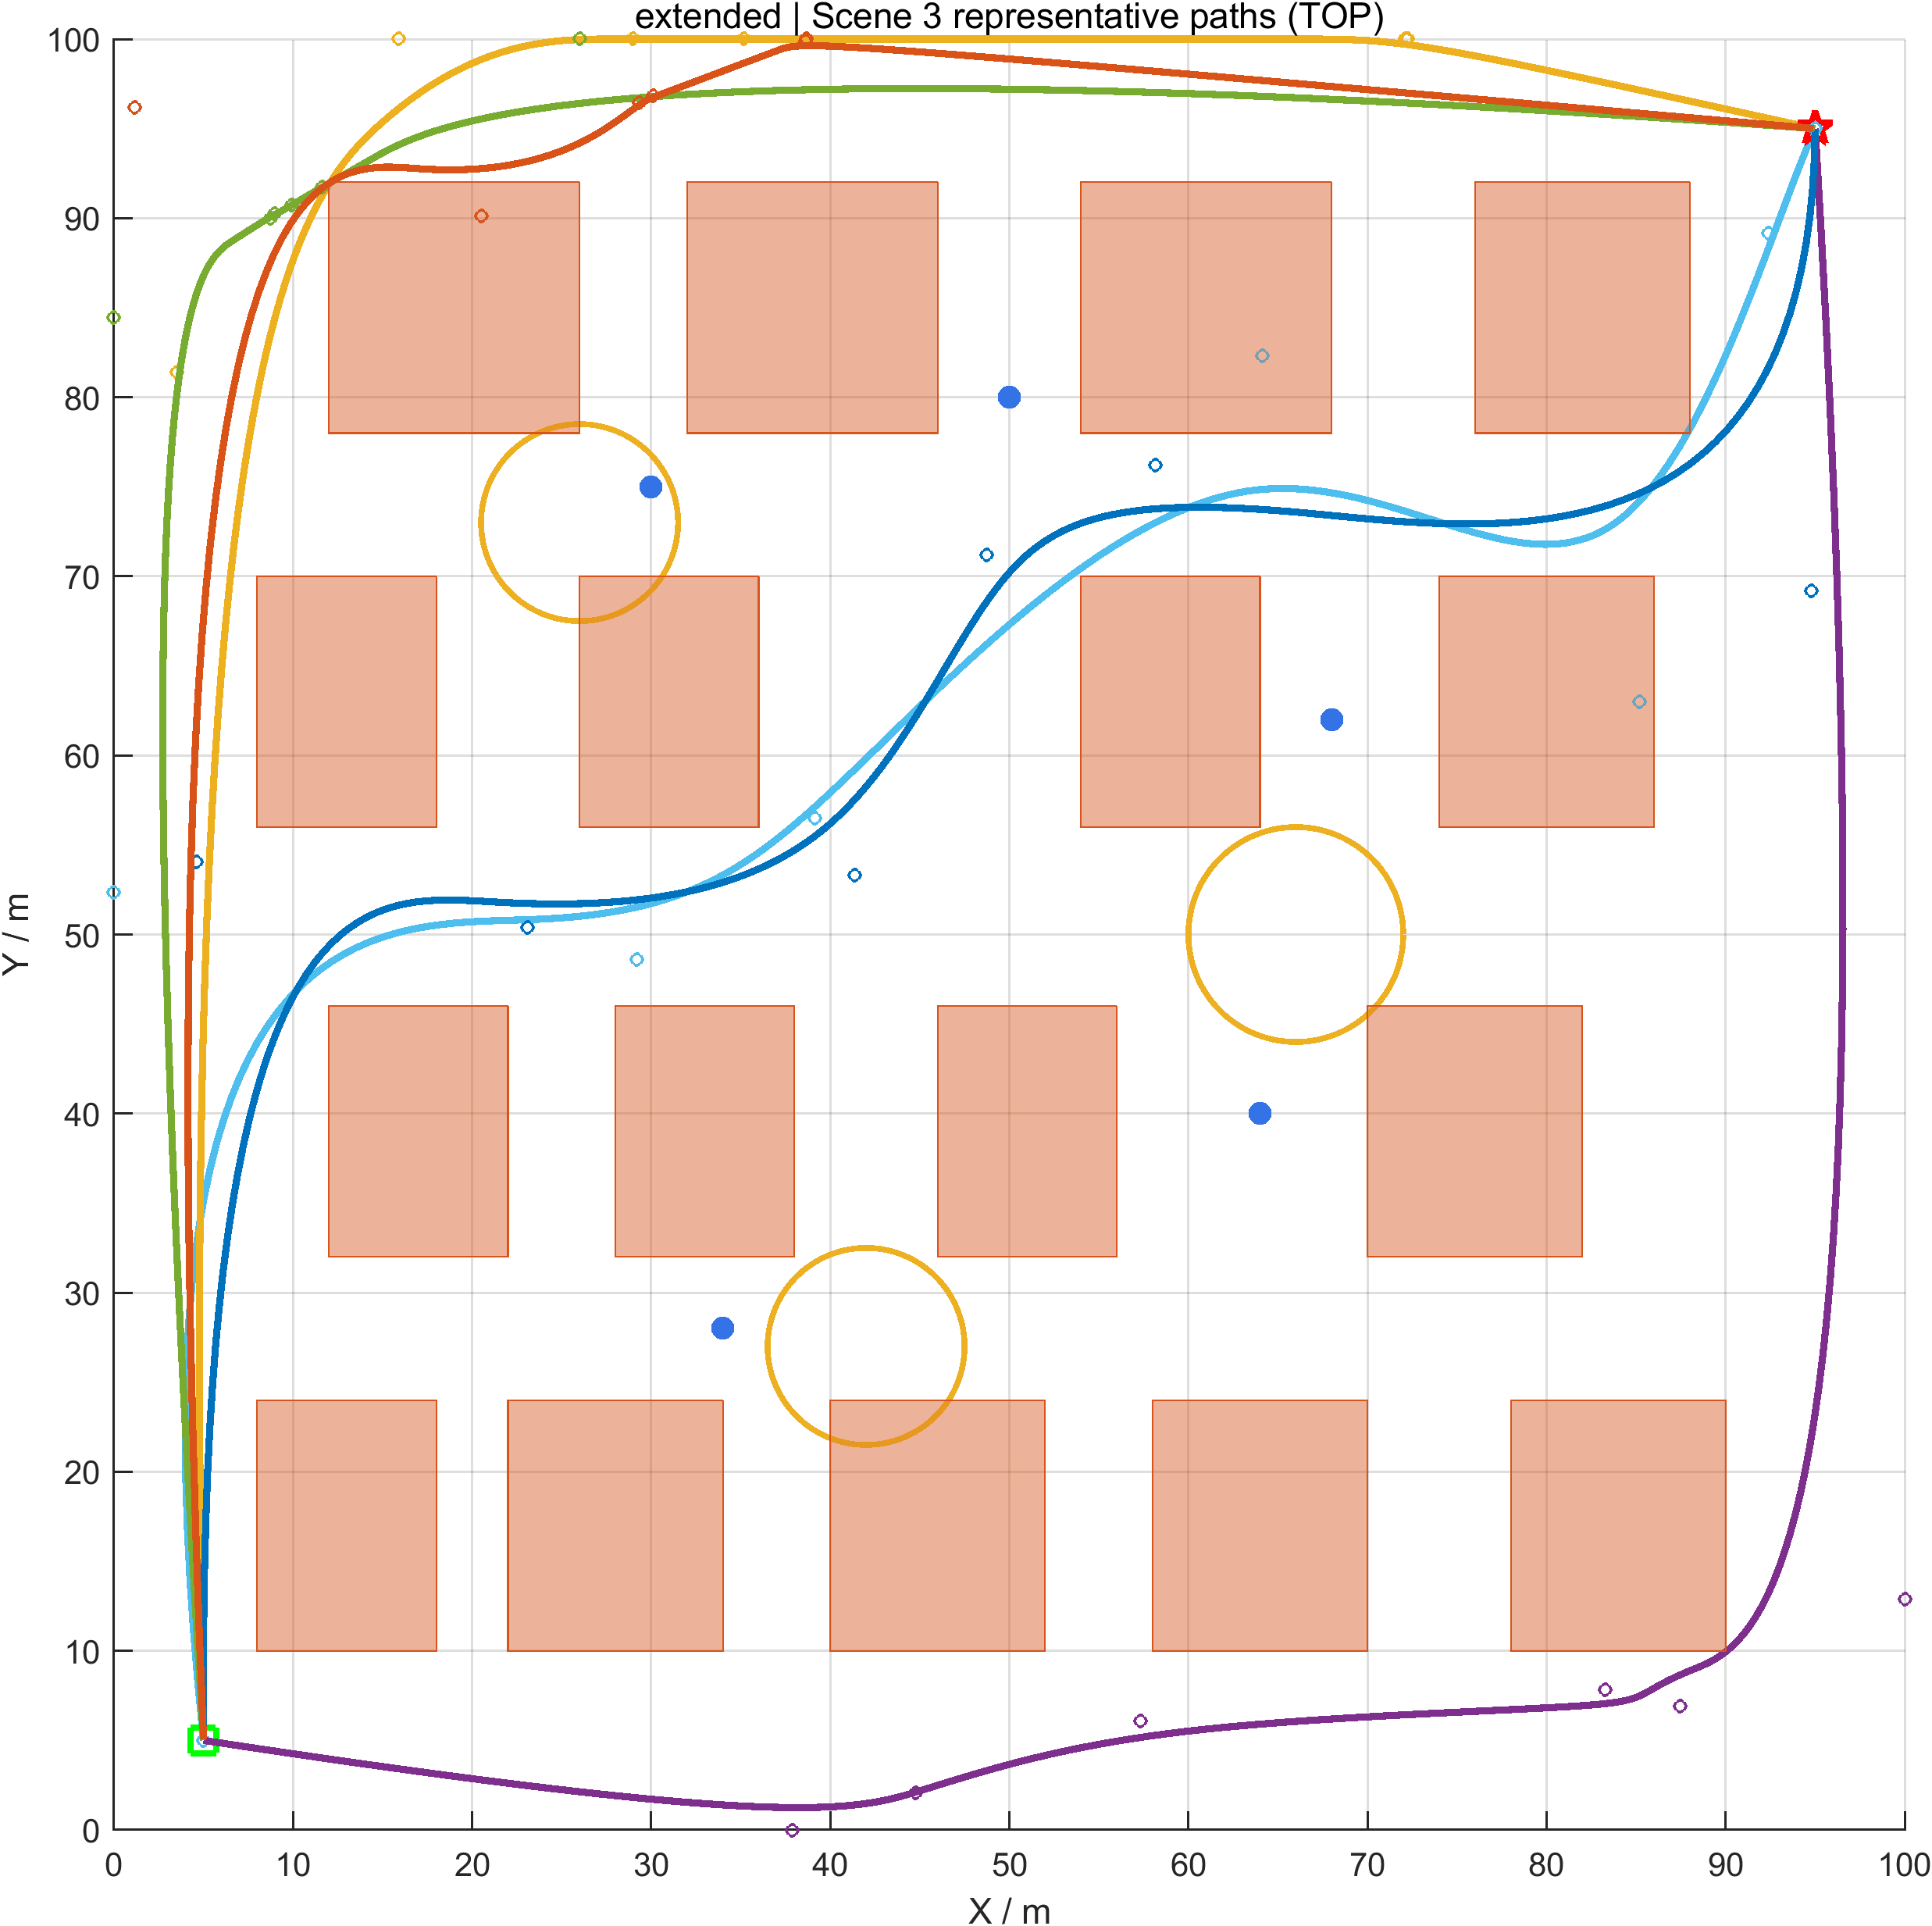
\includegraphics[width=\linewidth]{extended_scene3_representative_top.png}
    \caption{Scene 3}
\end{subfigure}
\caption{三类测试场景的代表性路径俯视对比}
\label{fig:extended-paths-top}
\end{figure*}

\begin{figure*}[tbp]
\centering
\begin{subfigure}{0.32\linewidth}
    \centering
    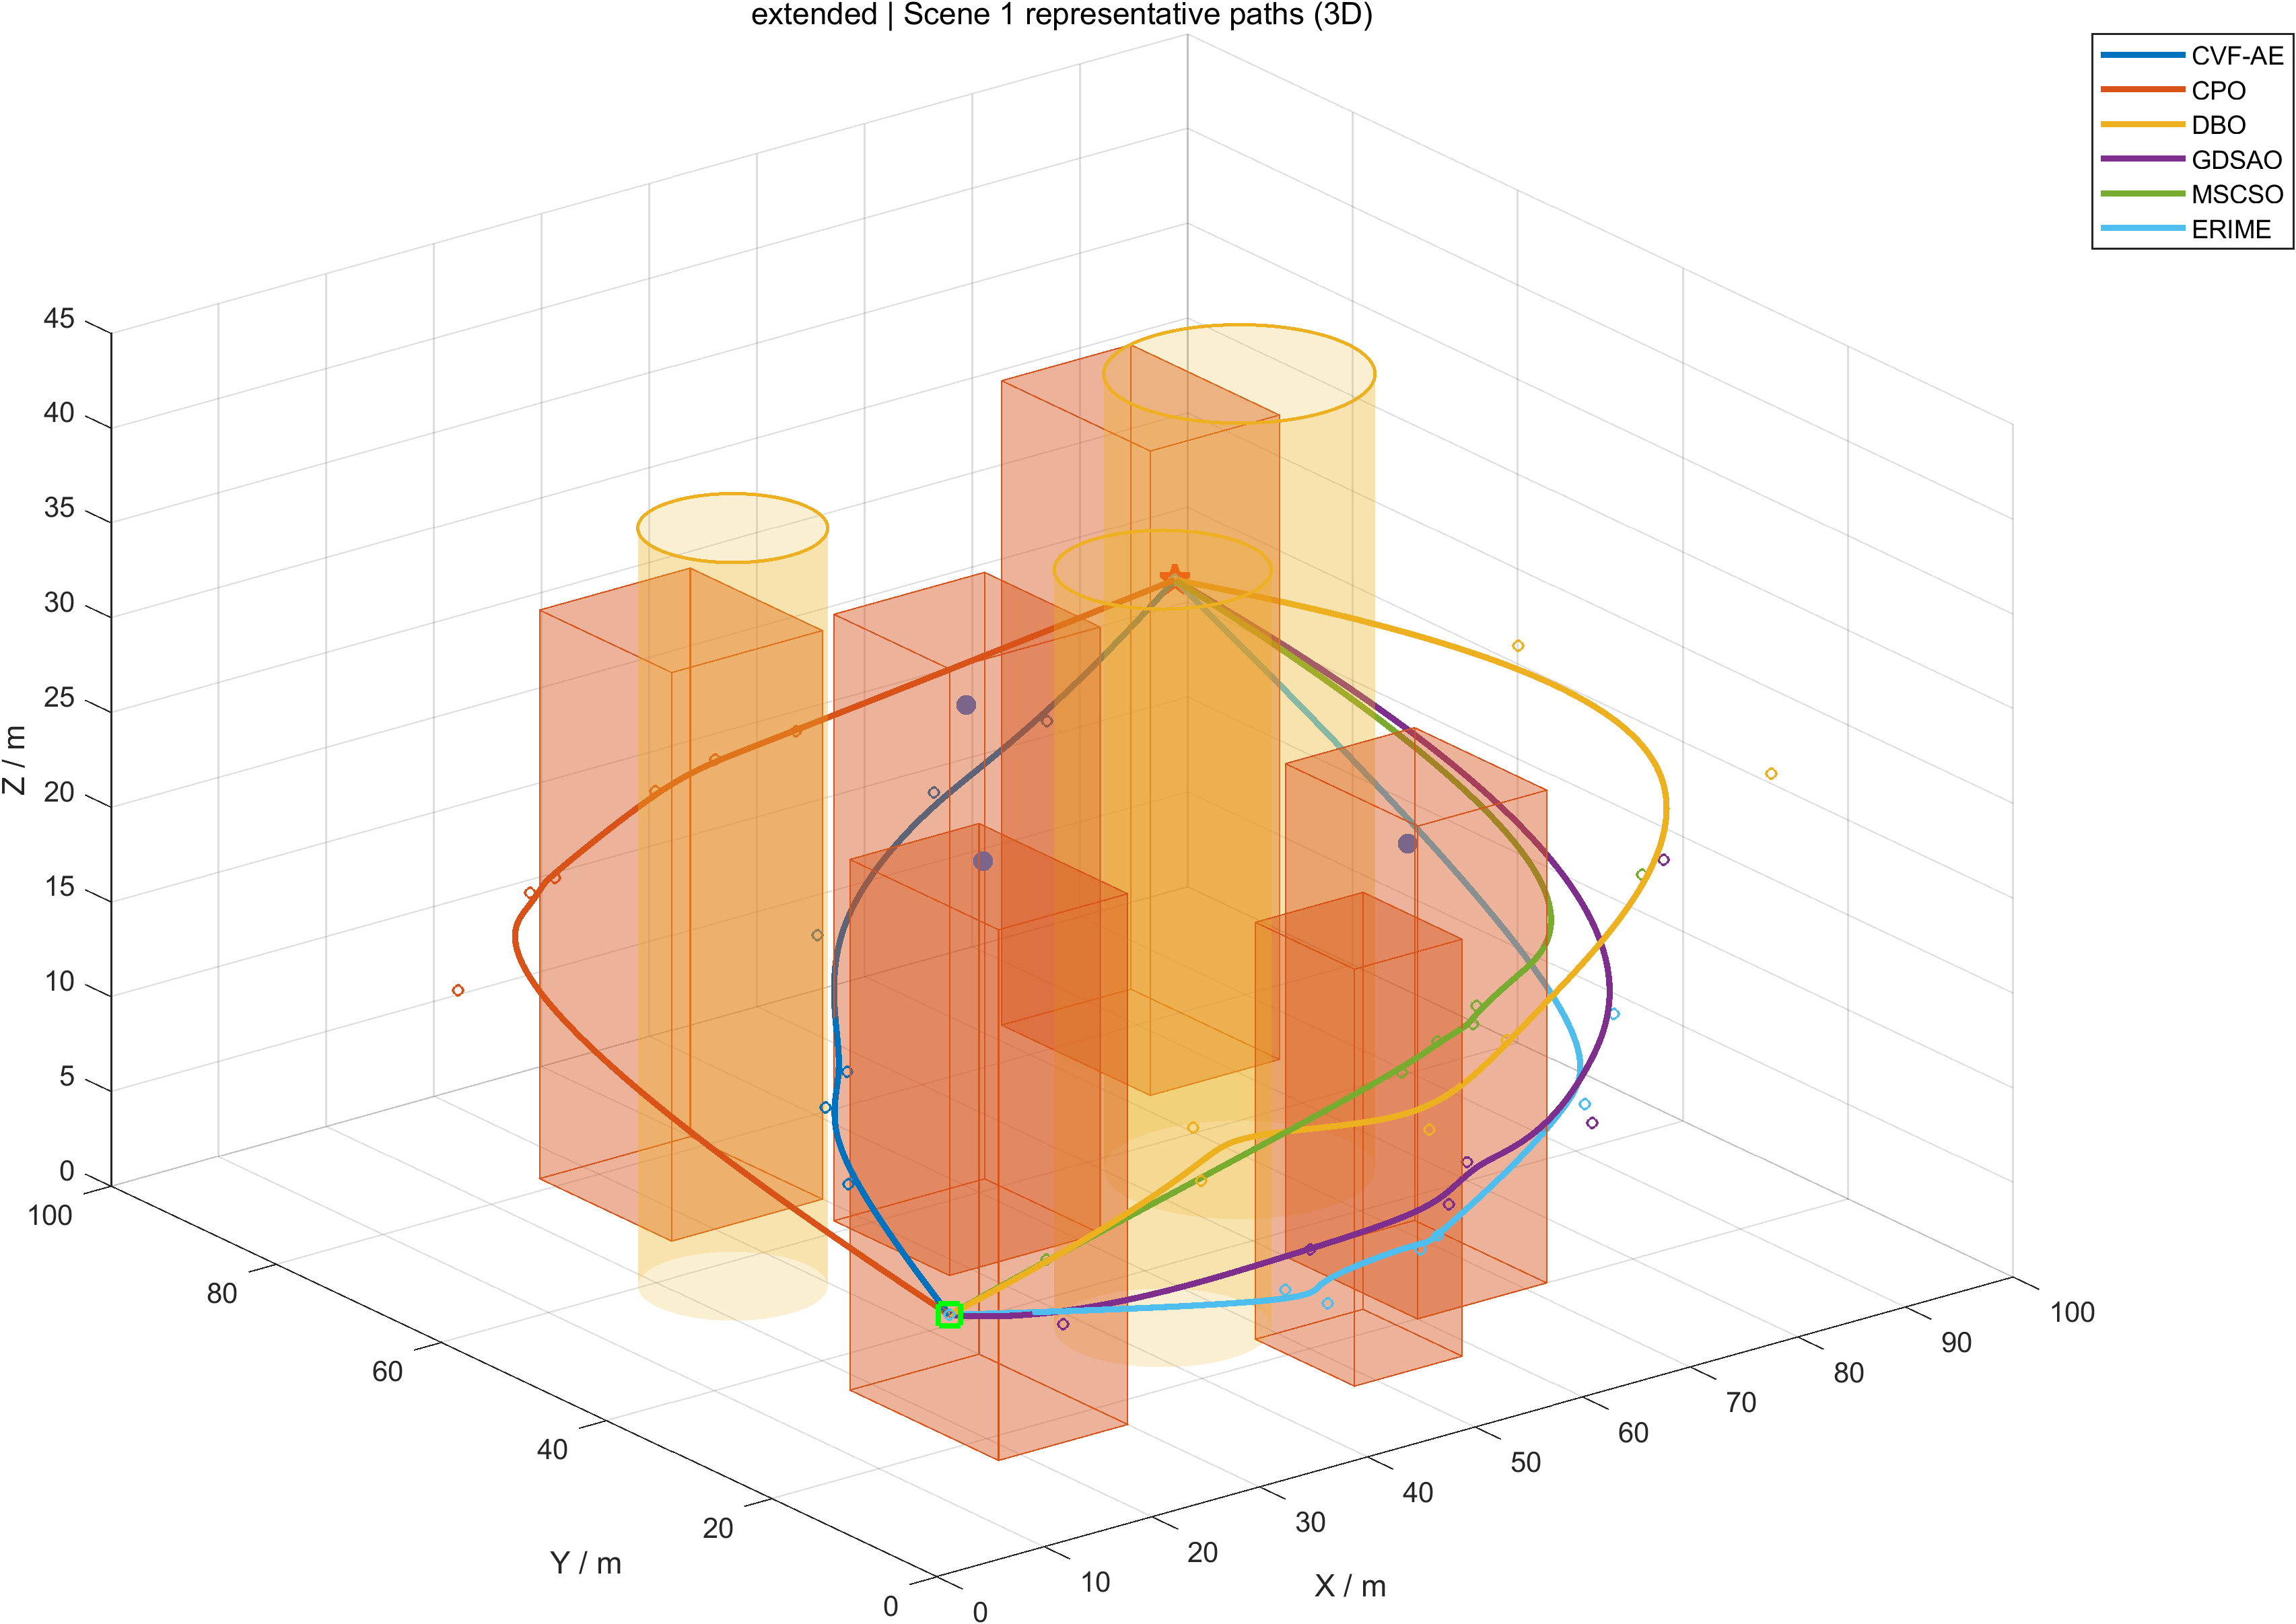
\includegraphics[width=\linewidth]{extended_scene1_representative_3d.png}
    \caption{Scene 1}
\end{subfigure}
\hfill
\begin{subfigure}{0.32\linewidth}
    \centering
    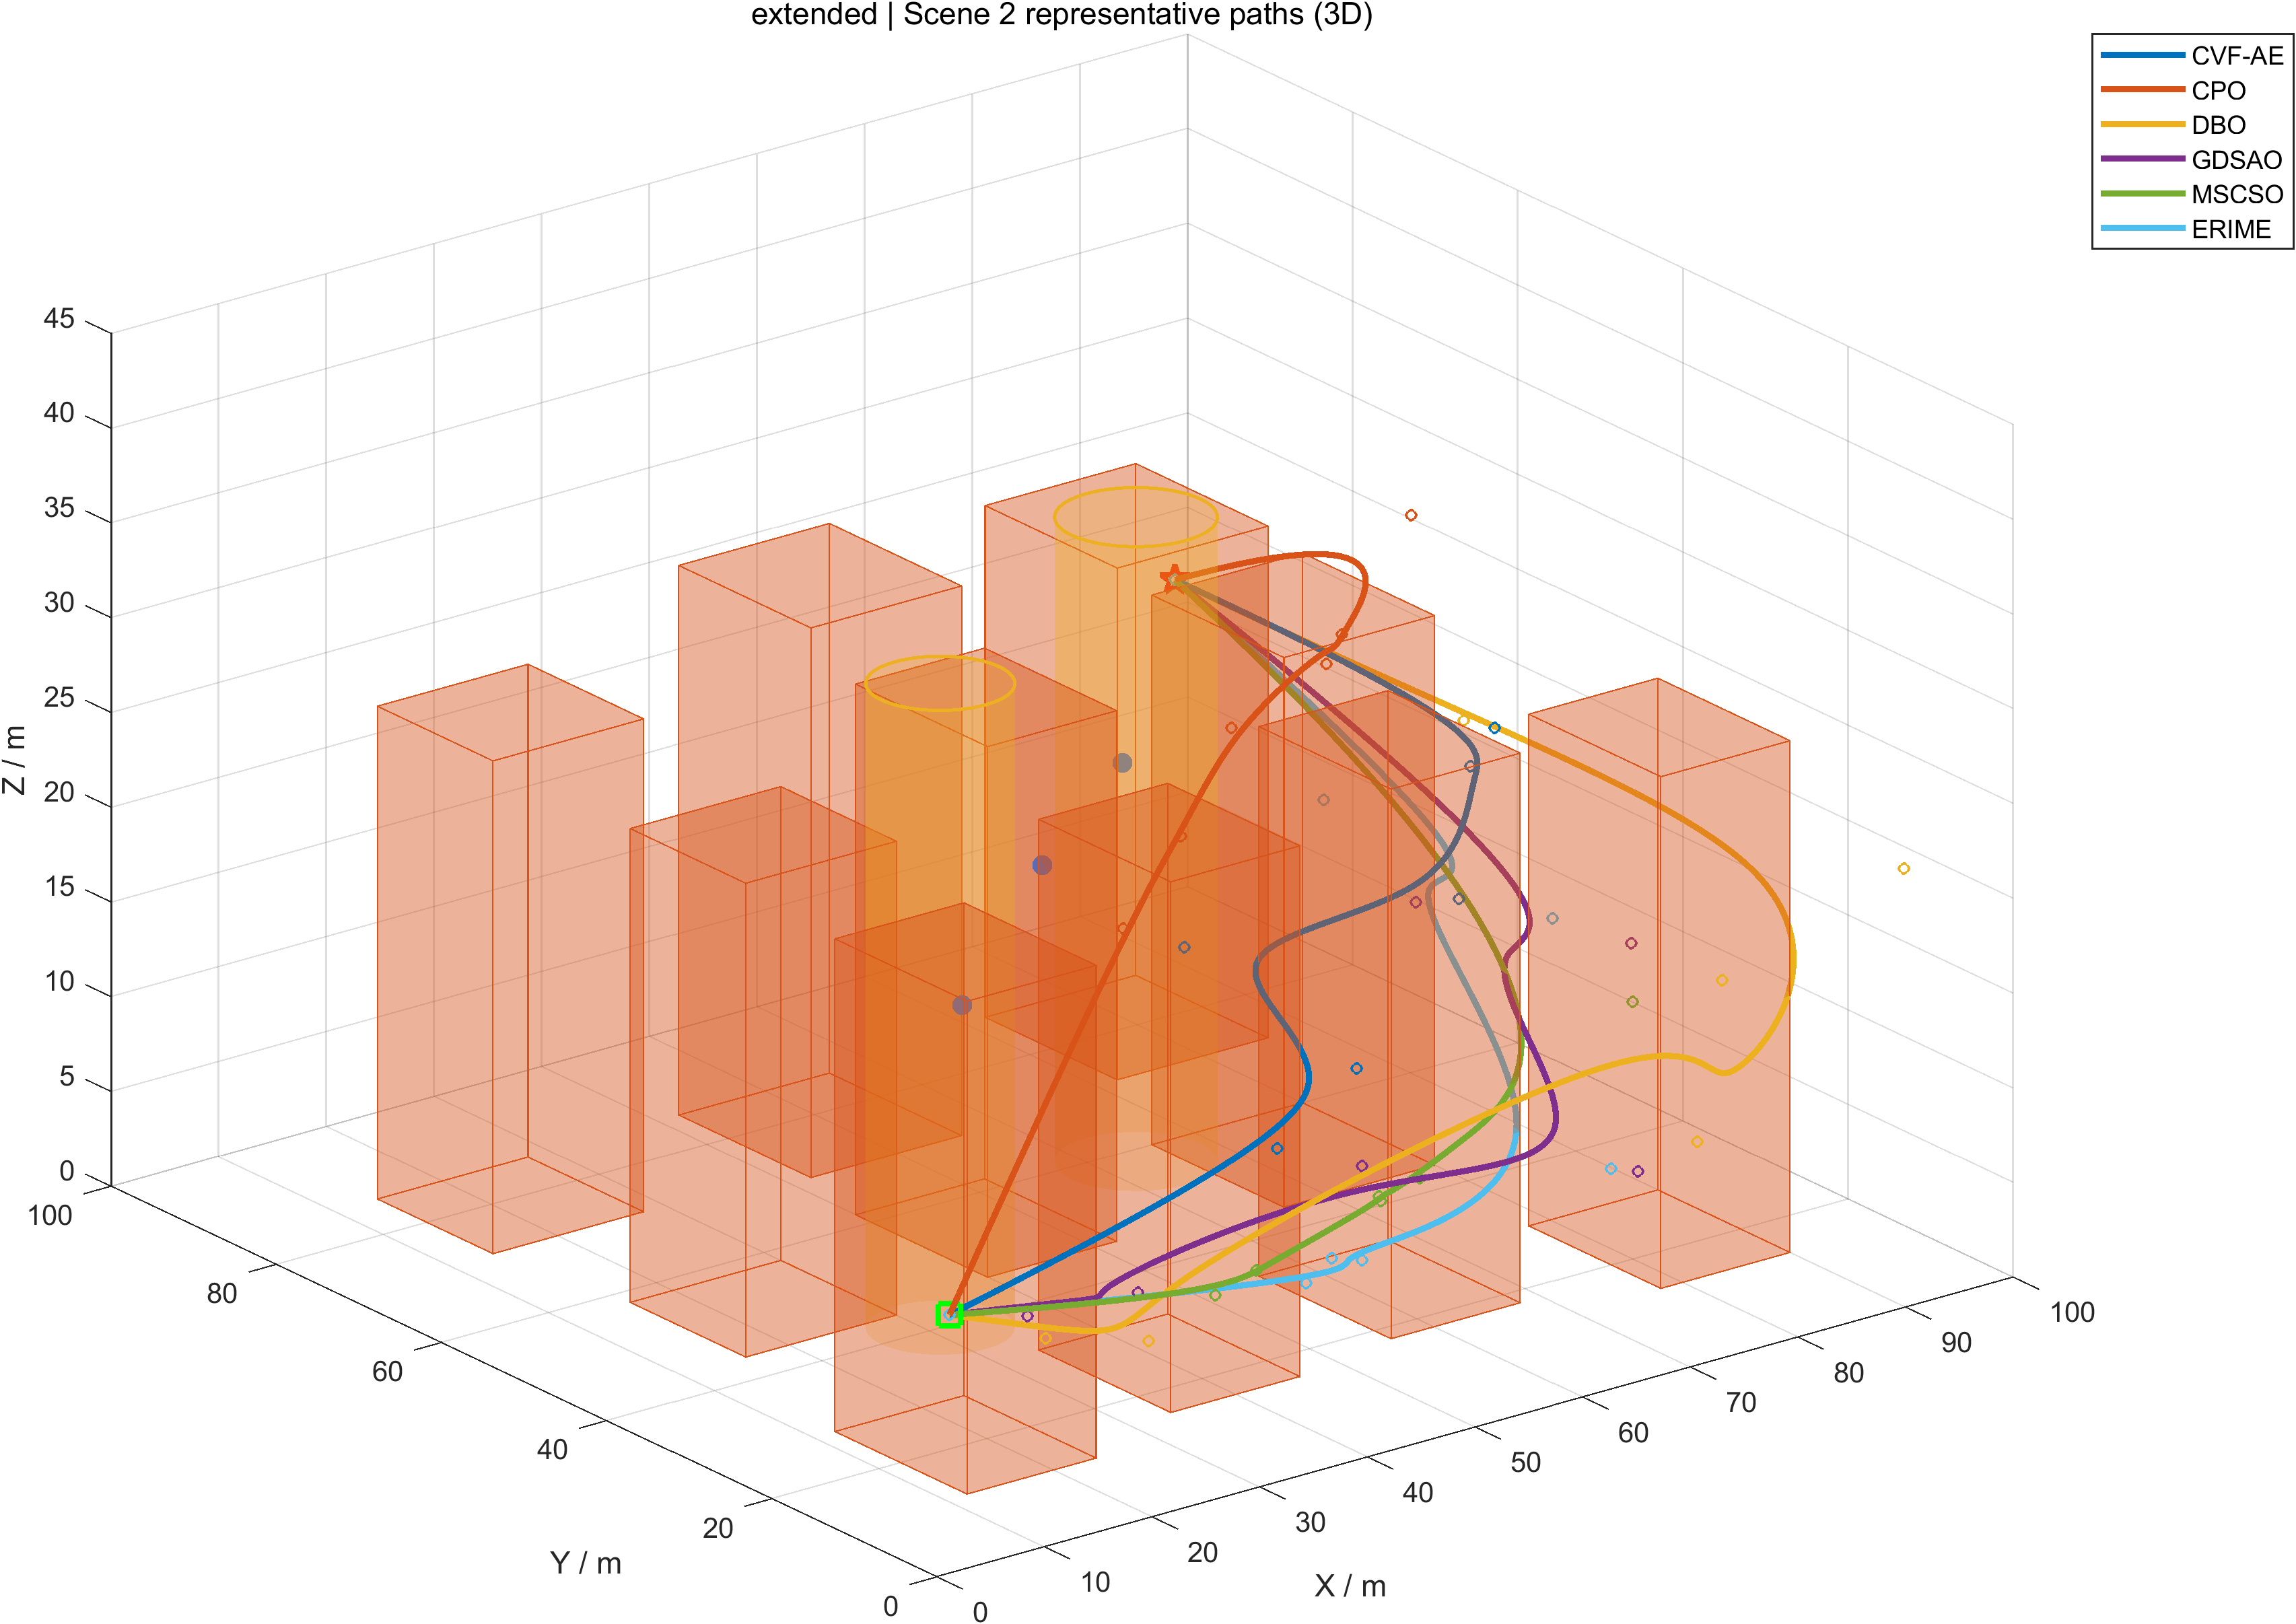
\includegraphics[width=\linewidth]{extended_scene2_representative_3d.png}
    \caption{Scene 2}
\end{subfigure}
\hfill
\begin{subfigure}{0.32\linewidth}
    \centering
    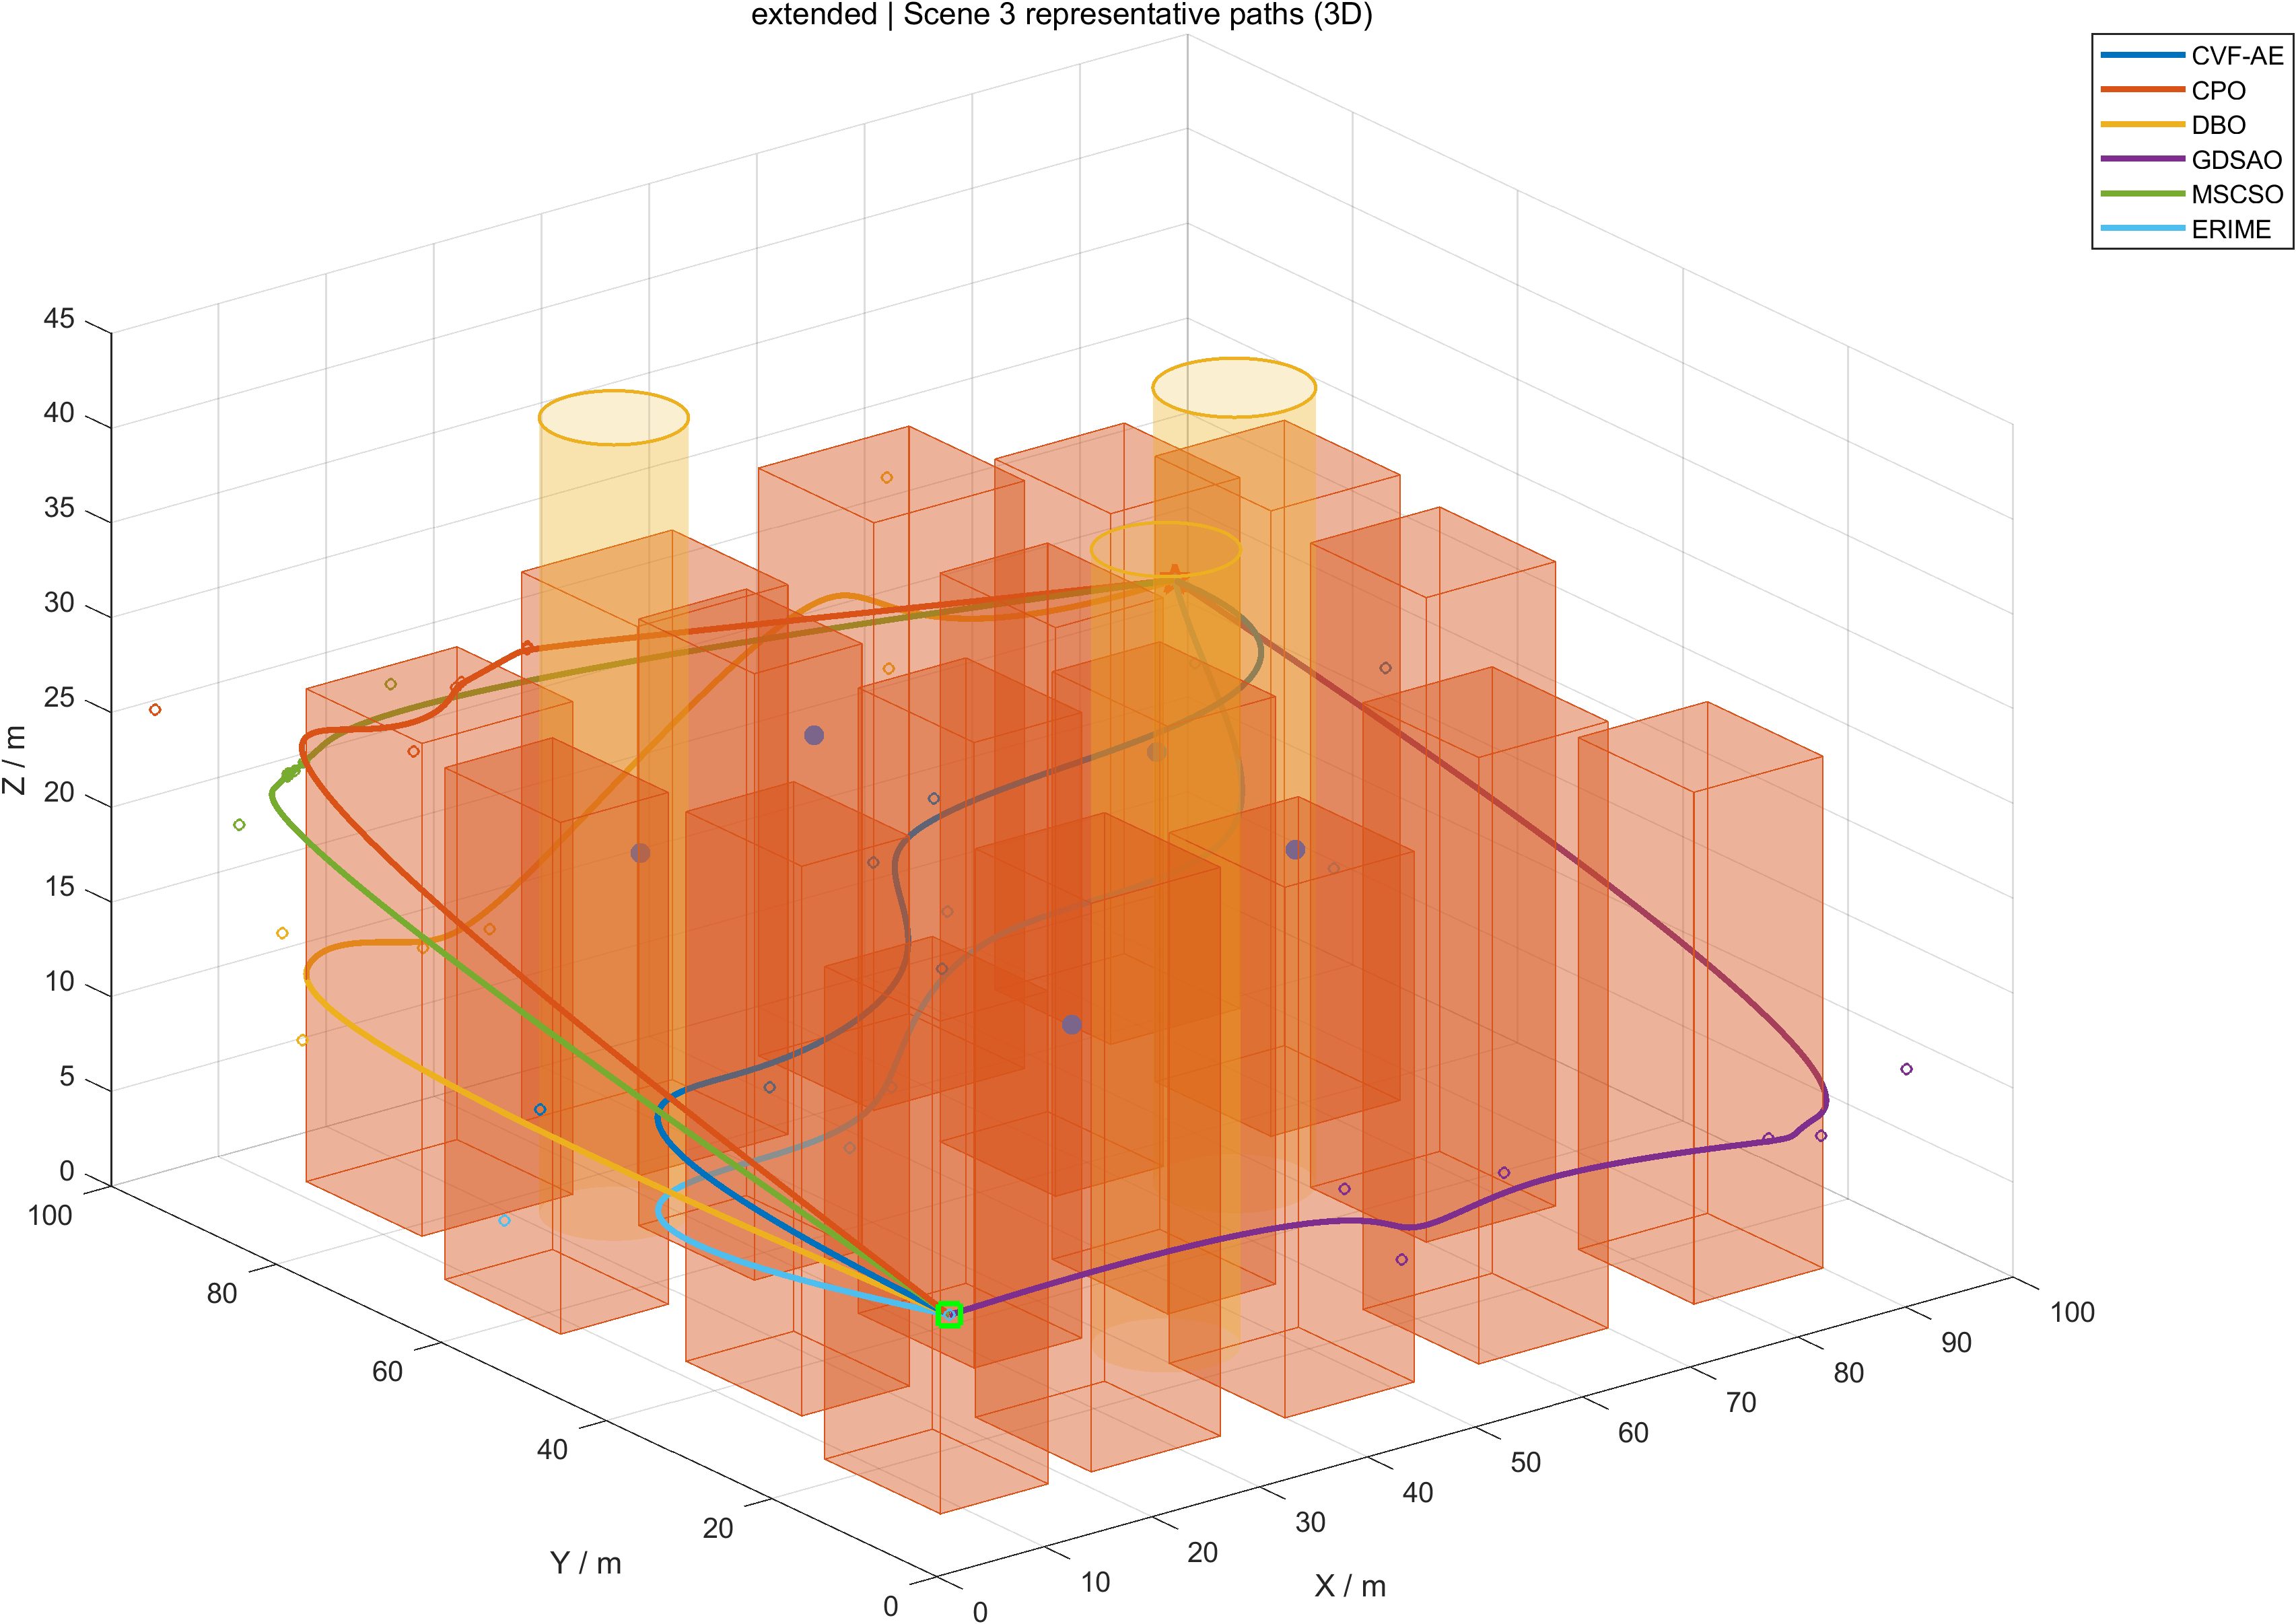
\includegraphics[width=\linewidth]{extended_scene3_representative_3d.png}
    \caption{Scene 3}
\end{subfigure}
\caption{三类测试场景的代表性路径三维对比}
\label{fig:extended-paths-3d}
\end{figure*}

\subsection{消融实验}

\begin{table*}[tbp]
\centering
\caption{CVF-AE 关键模块消融实验结果}
\label{tab:ablation}
\setlength{\tabcolsep}{3pt}
\tiny
\resizebox{\textwidth}{!}{%
\begin{tabular}{clcccccc}
\toprule
Scene & Variant & $J$ & FR & R & Avg. R & nEvals & CVF trig./succ. \\
\midrule
1 & CVF-AE & 297.8318 $\pm$ 3.1119 & 1.00 & 1 & 1.00 & 9566.4 & 21.1/19.2 \\
1 & CVF-AE-w/o-CVF & 306.1985 $\pm$ 3.4917 & 1.00 & 3 & 3.00 & 9471.8 & 0.0/0.0 \\
1 & CVF-AE-w/o-StateAdaptiveCVF & 298.3037 $\pm$ 3.2161 & 1.00 & 2 & 2.33 & 9566.0 & 20.6/19.7 \\
1 & CVF-AE-w/o-SparsePreservation & 306.3793 $\pm$ 4.9973 & 1.00 & 4 & 3.67 & 9140.1 & 110.1/90.7 \\
1 & CVF-AE-w/o-Init & 316.9964 $\pm$ 11.8481 & 1.00 & 5 & 5.00 & 9587.6 & 140.2/93.1 \\
1 & Base-AE & 654.0475 $\pm$ 328.7142 & 0.63 & 6 & 6.00 & 9030.0 & 0.0/0.0 \\
2 & CVF-AE & 300.6612 $\pm$ 3.2775 & 1.00 & 1 & 1.00 & 9551.6 & 10.6/7.9 \\
2 & CVF-AE-w/o-CVF & 303.7697 $\pm$ 4.9565 & 1.00 & 4 & 3.00 & 9432.5 & 0.0/0.0 \\
2 & CVF-AE-w/o-StateAdaptiveCVF & 301.8164 $\pm$ 2.9332 & 1.00 & 2 & 2.33 & 9560.9 & 20.4/14.6 \\
2 & CVF-AE-w/o-SparsePreservation & 303.3114 $\pm$ 6.0718 & 1.00 & 3 & 3.67 & 9107.8 & 77.8/51.5 \\
2 & CVF-AE-w/o-Init & 313.2191 $\pm$ 18.3412 & 1.00 & 5 & 5.00 & 9592.4 & 153.7/107.4 \\
2 & Base-AE & 1597.4829 $\pm$ 342.4791 & 0.00 & 6 & 6.00 & 9030.0 & 0.0/0.0 \\
3 & CVF-AE & 348.5856 $\pm$ 21.8153 & 1.00 & 1 & 1.00 & 9367.1 & 86.8/59.5 \\
3 & CVF-AE-w/o-CVF & 355.8347 $\pm$ 21.3086 & 1.00 & 2 & 3.00 & 9258.5 & 0.0/0.0 \\
3 & CVF-AE-w/o-StateAdaptiveCVF & 361.3123 $\pm$ 35.0403 & 1.00 & 3 & 2.33 & 9321.8 & 72.5/46.3 \\
3 & CVF-AE-w/o-SparsePreservation & 372.2255 $\pm$ 19.8216 & 1.00 & 4 & 3.67 & 9118.7 & 88.7/56.6 \\
3 & CVF-AE-w/o-Init & 556.7515 $\pm$ 348.8264 & 0.70 & 5 & 5.00 & 9802.7 & 417.9/336.5 \\
3 & Base-AE & 1643.7320 $\pm$ 199.4027 & 0.00 & 6 & 6.00 & 9030.0 & 0.0/0.0 \\
\bottomrule
\end{tabular}%
}
\vspace{1mm}
\parbox{\textwidth}{\footnotesize 注：FR 为可行率，R 为场景内排名，Avg. R 为跨场景平均排名。CVF trig./succ. 表示平均触发的 CVF 候选数 / 平均被局部接收的 CVF 候选数。}
\end{table*}


表 \ref{tab:ablation} 展示了正式消融实验结果。完整 CVF-AE 在三个场景中的消融平均排名为 $1.00$，并在所有场景保持 $1.00$ 的可行率。与 Base-AE 相比，完整方法在 Scene 2 和 Scene 3 中将可行率从 $0$ 提升到 $1.00$，说明仅依靠基础 AE 搜索无法稳定穿越强约束低空场景，而约束感知初始化、CVF 候选和稀疏保持机制共同提高了可行路径形成能力。

图 \ref{fig:ablation-scene2-top} 和图 \ref{fig:ablation-scene3-3d} 展示了完整方法与消融版本的路径形态差异。Scene 2 的俯视图说明完整方法更稳定地沿低风险可行走廊推进；去除关键模块后，路径更容易出现绕行、靠近障碍或需要更多后处理修复。Scene 3 的三维图进一步补充高度维度证据：由于高度上界更低、障碍和禁飞区更密集，去除初始化或 CVF 相关机制后，算法更容易依赖较差的空间绕行或停留在低质量可行区域。两图与表 \ref{tab:ablation} 中 Scene 3 的适应度和可行率变化相互印证。

\begin{figure}[tbp]
\centering
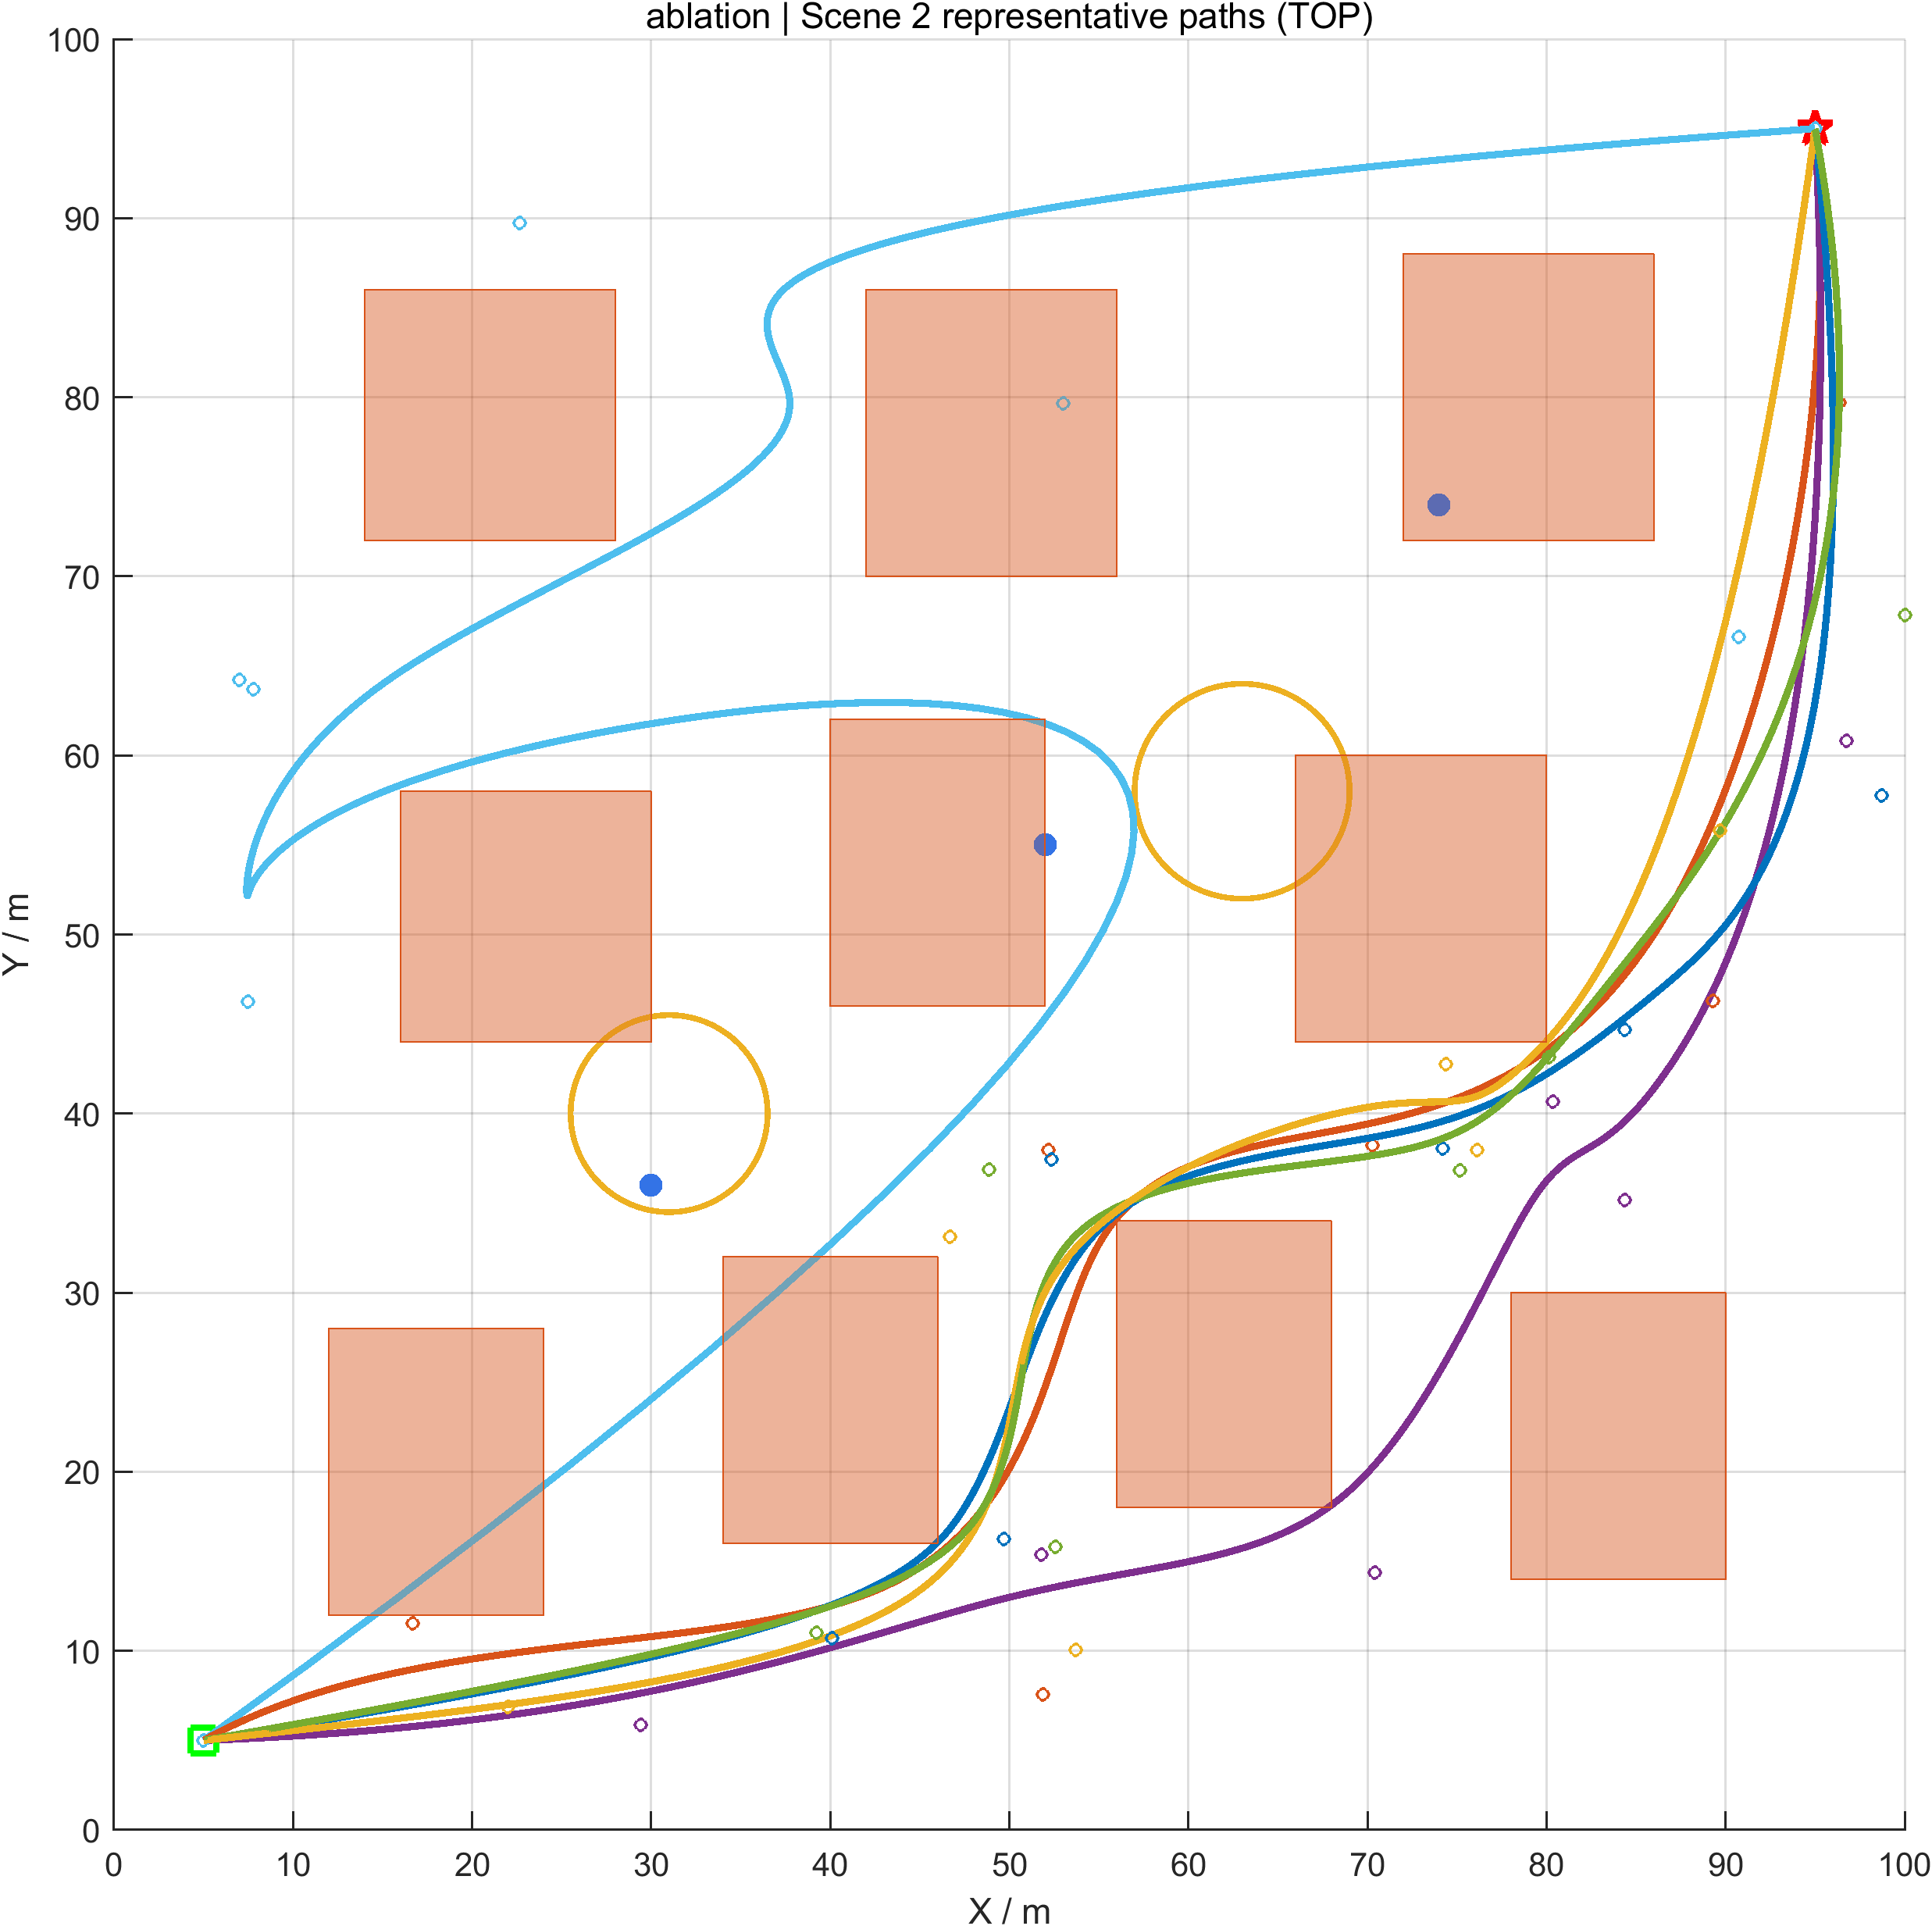
\includegraphics[width=0.78\linewidth]{ablation_scene2_representative_top.png}
\caption{Scene 2 关键模块消融版本的代表性路径俯视对比}
\label{fig:ablation-scene2-top}
\end{figure}

\begin{figure}[tbp]
\centering
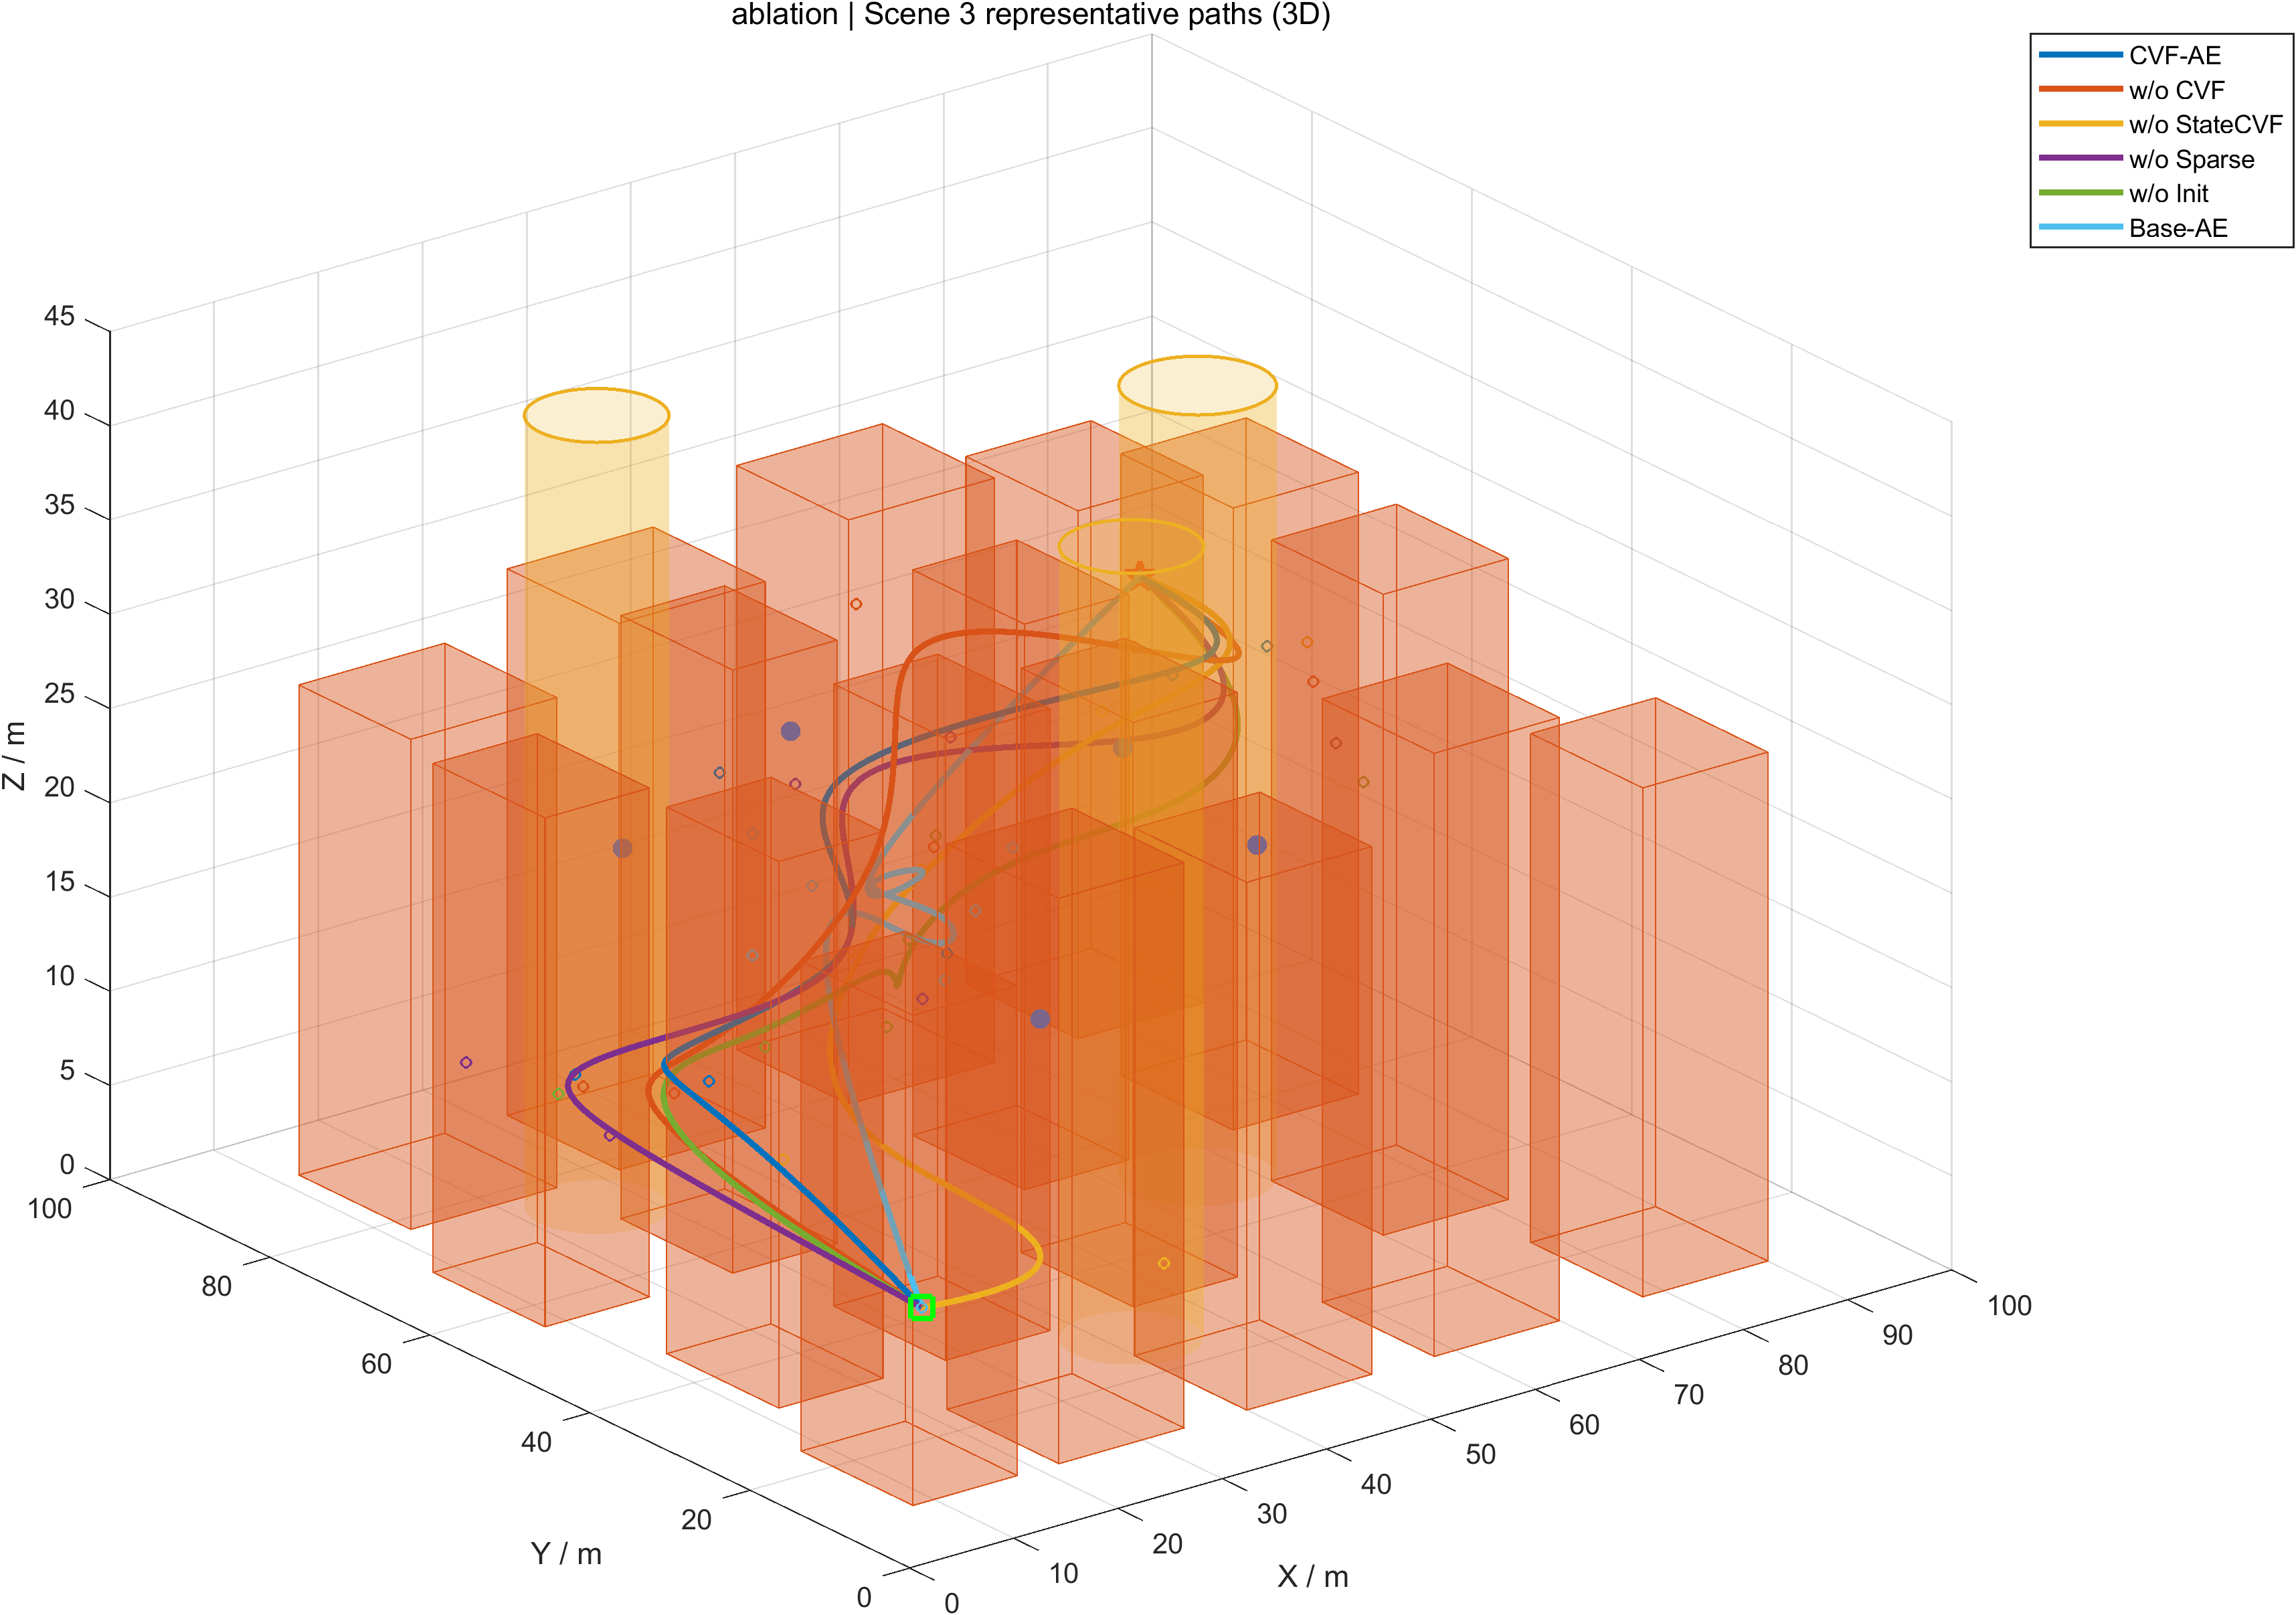
\includegraphics[width=0.78\linewidth]{ablation_scene3_representative_3d.png}
\caption{Scene 3 关键模块消融版本的代表性路径三维对比}
\label{fig:ablation-paths}
\label{fig:ablation-scene3-3d}
\end{figure}

去除 CVF 场后，算法在三个场景仍能保持可行，但适应度均有所上升：Scene 1 从 $297.8318$ 上升到 $306.1985$，Scene 2 从 $300.6612$ 上升到 $303.7697$，Scene 3 从 $348.5856$ 上升到 $355.8347$。这说明在已有初始化和 repair 支撑下，CVF 不是唯一可行性来源，但能够在可行区域附近提供额外的方向引导，使路径质量进一步改善。

去除约束感知初始化的影响在 Scene 3 最明显，可行率从 $1.00$ 降至 $0.70$，平均适应度升至 $556.7515$，并伴随更多 CVF 触发。这表明初始化并不是简单加速技巧，而是强约束走廊中避免搜索长期滞留不可行区域的重要组成部分。去除稀疏保持机制后，三个场景的适应度均弱于完整方法，说明局部修复与可行性保持对路径稳定性仍有贡献。

状态自适应 CVF 的作用更细致。消融均值显示，去除状态自适应 CVF 后并非每个场景都明显劣化，这意味着状态调度不宜被解释为单独决定性能的模块。更稳妥的解释是：状态自适应、CVF 场、初始化和稀疏保持在不同约束阶段形成互补，完整机制在总体上保持最稳定的综合表现。

\subsection{评价开销与参数稳健性}

\begin{table}[tbp]
\centering
\caption{CVF-AE 评价开销与稀疏触发统计}
\label{tab:runtime}
\tiny
\resizebox{\columnwidth}{!}{%
\begin{tabular}{@{}lcccccc@{}}
\toprule
Group & Sc. & nEvals & Trig. & Succ. & Rate & Ratio \\
\midrule
Main & 1 & 9569.5 & 25.0 & 22.4 & 0.28\% & -- \\
Main & 2 & 9552.7 & 12.4 & 9.5 & 0.14\% & -- \\
Main & 3 & 9362.5 & 83.8 & 56.4 & 0.93\% & -- \\
\midrule
Abl. & 1 & 9566.4 & 21.1 & 19.2 & 0.22\% & 1.010 \\
Abl. & 2 & 9551.6 & 10.6 & 7.9 & 0.11\% & 1.013 \\
Abl. & 3 & 9367.1 & 86.8 & 59.5 & 0.93\% & 1.012 \\
\bottomrule
\end{tabular}%
}
\vspace{1mm}
\parbox{\columnwidth}{\footnotesize 注：Trig. 和 Succ. 分别表示平均触发的 CVF 候选数和平均被接收的 CVF 候选数；Ratio 为完整 CVF-AE 相对于同批次 w/o-CVF 消融版本的评价次数比。}
\end{table}


表 \ref{tab:runtime} 给出了 CVF-AE 的评价开销摘要。主对比中，CVF-AE 在 Scene 1、Scene 2 和 Scene 3 的平均评价次数分别为 $9568.9$、$9554.2$ 和 $9355.2$，与 $N=30$、$T=300$ 的基础评价规模接近。CVF 触发次数在 Scene 1 和 Scene 2 分别为 $23.9$ 和 $13.1$，对应触发率低于 $0.3\%$；在更强约束的 Scene 3 中，触发次数增至 $88.6$，触发率仍低于 $1\%$。该趋势与方法设计一致：当约束更密集、可行走廊更窄时，稀疏 CVF 分支会更频繁地被触发，但不会退化为全种群强制更新。

同批次消融对比显示，完整 CVF-AE 相对于去除 CVF 的版本，在三个场景中的评价次数比值约为 $1.010$、$1.013$ 和 $1.012$。这支持“额外评价次数受控”的结论。本文不将绝对 wall-clock time 作为主要效率证据，因为 MATLAB 运行时间会受到 repair 次数、路径可行形成速度、会话状态和批处理负载影响。更合理的结论是：CVF-AE 的额外评价开销约为 $1\%$ 量级，低开销主要来自稀疏触发和局部候选接收，而不是来自更短的绝对运行时间。

参数稳健性检查进一步作为补充说明使用，而不作为独立性能证据。候选触发配额、CVF 步长强度和保守状态切换阈值的小范围扰动显示：更高触发配额可在 Scene 2 和 Scene 3 中降低部分适应度均值，但会增加触发次数和额外评价规模；步长强度的较优档位随场景变化；状态切换阈值没有在两个检查场景上同时稳定占优的非默认设置。因此，本文保留默认参数，并将结论限定为默认配置具有较好的折中稳健性，而不是依赖单一场景调参获得优势。

\subsection{综合讨论}

综合主对比、显著性、消融、开销和参数稳健性分析，CVF-AE 的价值主要体现在三个方面。第一，在所测试的三类合成低空场景中，它保持 $1.00$ 的可行率，并在扩展主对比中获得最佳平均排名，说明约束可行性场与可行性优先准则能够稳定服务于本文设定的强约束路径规划任务。第二，它在 Scene 2 和 Scene 3 这类更强约束场景中提供了比多数基线更均衡的路径，不以高空绕行或边界贴靠作为主要代价。第三，稀疏触发使 CVF 额外评价次数保持在较低水平，避免了每代全种群构造可行性场所带来的计算膨胀。

本文的结论也有明确边界。CVF-AE 不是每个场景的最低标量适应度算法；Scene 2 中 CPO 和 MSCSO 的适应度显著更低，Scene 3 中 GDSAO 的均值也略低于 CVF-AE。本文将这些结果解释为低空 UAV 路径规划中的多指标折中：最终适应度、可行率、轨迹复核风险和评价开销必须共同考虑。基于这一口径，CVF-AE 在强约束低空路径规划任务中表现为更均衡、更稳定的工程型优化方法。

\subsection{局限性与未来工作}
\label{sec:limitations}

本文仍存在若干限制。首先，实验场景为静态合成低空环境，主要用于验证强约束三维路径规划中的可行性形成、轨迹质量和评价开销，尚未引入真实地图、DEM 数据或城市级障碍物建模。其次，当前任务假设障碍物和禁飞区在规划周期内保持不变，尚未覆盖动态障碍、在线重规划或多无人机协同避碰。再次，当前实现对不可行解采用实现相关违反分数排序，并使用保守局部 CVF 候选接收规则；归一化违反量、安全优先词典序或更激进的可行性改善接收均属于后续算法变体，需要重新开展正式实验。最后，本文评估对象为路径规划层面的几何可行性和优化性能，尚未与飞控约束、动力学模型和轨迹跟踪控制器进行闭环联调。后续工作可在真实地形数据、动态低空交通约束和控制器可跟踪性验证中进一步检验 CVF-AE 的工程适用性。

\section{结论}
\label{sec:conclusion}

本文面向强约束三维低空无人机路径规划问题，提出了约束可行性场驱动的自适应进化搜索方法 CVF-AE。该方法通过约束感知初始化、局部 CVF 候选引导、状态自适应触发和稀疏可行性保持，将约束违反信息用于低开销的方向修正，而不是在每一代对全种群进行强制更新。

三类合成低空场景实验表明，CVF-AE 在所测试场景中保持稳定可行性，并在主对比中取得最佳平均排名。统计检验和轨迹复核进一步说明，本文方法的优势主要体现在可行率、轨迹合理性和评价开销之间的均衡，而不是保证每个场景都获得最低标量适应度。消融结果验证了 CVF、约束感知初始化和稀疏保持机制在强约束环境中的互补作用；评价开销结果则表明，CVF 分支以稀疏方式触发，额外评价次数保持在约 $1\%$ 量级。

总体而言，CVF-AE 为强约束低空路径规划提供了一种可解释、可控开销的工程型进化优化框架。后续研究将围绕真实地形环境、动态障碍约束以及规划--控制闭环验证进一步扩展。


\section*{致谢}
基金、致谢和作者声明内容待补。

\section*{利益冲突}
利益冲突声明待补。

\section*{数据可用性声明}
数据可用性声明待补。

\bibliographystyle{unsrtnat}
\bibliography{bib/references}

\end{document}
